\documentclass[11pt]{article}
\usepackage[letterpaper, margin=1in]{geometry}

\usepackage{natbib}         % cite references
\usepackage{multibib}
\newcites{rev}{References}  % citep --> citeprev; citet --> citetrev

%\usepackage[sectionbib]{chapterbib} 
\usepackage[utf8]{inputenc}       % noindent
\usepackage[dvipsnames]{xcolor}   % use colors
\usepackage{authblk}              % author names
\usepackage{ragged2e}             % align text
\usepackage{booktabs}             % use tables
\usepackage{graphicx}             % using figures
\usepackage{caption}              % no caption numbers for figures in responses
\usepackage{amsthm}   % use mathematics
\usepackage{soul}     % wrapped underline 

\usepackage{xr-hyper} % use cross references in two tex files
\externaldocument{materials} % link the external document
\externaldocument{02-revise} % link the external document
\usepackage{hyperref} % use hyperlinks
\hypersetup{colorlinks=true, citecolor=black, linkcolor=black, urlcolor=blue}

% set the paper as noindent
\setlength\parindent{0pt}

% initialize counters for reviewer number and comment number
\newcounter{reviewer}
\setcounter{reviewer}{0}
\newcounter{point}[reviewer]
\setcounter{point}{0}

% set the format of reviewer comment numbers and responses
%% point
\renewcommand{\thepoint}{Comment\,\thereviewer.\arabic{point}:} 
\newcommand{\point}[1]{\refstepcounter{point} \bigskip \noindent {\fontseries{b}\selectfont \thepoint} #1 \par}
%% response
\newcommand{\sect}[1]{{\bigskip \bigskip \textbf{\noindent #1} }} % for section 
\newcommand{\reply}[1]{\bigskip \textcolor{blue}{\noindent \textbf {Reply:} #1}}
\newcommand{\nextreply}[1]{\bigskip \textcolor{blue}{\noindent #1}}
\newcommand{\marked}[1]{\bigskip \textit{\textcolor{blue}{\noindent #1}}}
\newcommand{\revised}[3][2]{\bigskip \textcolor{magenta}{\noindent \textbf{Line #2:} #3}}


% set the format for reviewer headings
\newcommand{\editorsection}{\newpage \section*{Editor} \hrule}
\newcommand{\reviewersection}{\newpage \stepcounter{reviewer} \section*{Reviewer \thereviewer} \hrule}

% set the format for to-do on in-progress responses
\newcommand\myTodo[1]{\textcolor{red}{! #1}}
% title page
\title{\raggedright {Response to Editors' and Reviewers' Comments:}
{\textbf{Climate and Cryosphere Cause Water Yield Regime Shifts in the Upper Brahmaputra River basin}}}
%%%%%%%%%%%%%%%%%%%%%%%%%%%%%%%%%%%%%%%%%%%%%%%%%%%%%%%%
\begin{document}
\date{}
\author{}
\maketitle

Dear Dr. Giulia Zuecco, \\

Thank you for giving us the opportunity to submit a revised draft of our manuscript, now entitled “Climate and Cryosphere Cause Water Yield Regime Shifts in the Upper Brahmaputra River basin” to Journal \textit{Hydrology and Earth System Sciences}. 
We appreciate the editors and reviewers for devoting their precious time to reviewing our paper and providing valuable suggestions. It was their insightful comments that have led to considerable improvements in the current version. \\

We have carefully considered your comments and incorporated the required changes, mainly including
(1) the schematic diagram explaining the DMC method used here, 
(2) detailed discussion about the results, especially "peak water", and potential implications on mountainous water resources management, and
(3) some limitations and uncertainties in the study. 
Moreover, the text has been carefully edited to improve the English writing and convey the results of the study more clearly. \\

Below we provide a point-by-point response to the comments and concerns from editors and reviewers. All modifications in the manuscript have been marked. \\

Sincerely

\begin{flushleft}
Hao Li (on behalf of all coauthors)  \\
PhD candidate, \url{Hao.liwork@ugent.be} \\
Hydro-Climate Extremes Lab, Ghent University \\
Jun 10, 2022 \\

\includegraphics[width=.15\textwidth]{02-figures/signature.png} \par
\end{flushleft}

%%%%%%%%%%%%%%
\editorsection
\point{Thank you for your responses to the comments provided by the reviewers. Both reviewers had major concerns about the manuscript, and they pointed out some key limitations. Specifically, the first reviewer observed that there is not enough information about the datasets, a clear explanation of the climate and cryosphere terms, and of the methodological approach used to differentiate the influence of climate, cryosphere and vegetation on the water yield. 
The second reviewer also asked to better address the cryosphere component (is it related only to the glacier ice melt or also to snowmelt and permafrost?), and to improve the discussion of the manuscript.
Furthermore, both reviewers suggested improving the discussion about the turning points that were found.
I carefully considered both the comments of the reviewers and your responses. Overall, I think that the responses to the first reviewer about the clarification of the two terms, climate and cryosphere, could have been more detailed, as well as the explanation of the methodological approach.
Besides the comments and suggestions of the two reviewers (that should be considered in the revision), I have the following recommendations that I would like to see implemented in the revised version of the manuscript.}
\reply{We are grateful the time and energy from Dr. Giulia Zuecco's and two reviewers in reviewing our manuscript. We have clarified your questions below and incorporated your suggestions into our revised manuscript, which improved significantly the quality of the manuscript. We sincerely hope that the revised version can satisfy the editors and reviewers.}

\point{Please move Table S1 in the main manuscript, and add details about the elevation ranges in the seven catchments, the main land use, and the percentage of glacier ice cover in each catchment (these details can be referred to a specific year, e.g. 2013 or 2015).}
\reply{Thanks for your suggestion. We have placed it in the main text, and added basic information, e.g. basin area, average elevation, hydrological stations, and the percentage of glacier and snow referred to 2000 land use and cover (Table \ref{tab: table 1}). The information will provide readers with a detailed introduction about our study region.}

\begin{table}[ht]
    \centering
    \caption{Information of six basins divided by the locations of hydrological stations.   
    The column "TP" indicates the turning point using the Pettitt method, in which a significant tuning point is labeled with *.
    Glaciers and snow area is acquired from the land use and cover in 2000 (see details in Dataset).}
    
    \begin{tabular}{ccccccc}
    \hline
    Abbrevation &
      Full names &
      Station &
      \begin{tabular}[c]{@{}c@{}}Total \\ area (km$^2$)\end{tabular} &
      \begin{tabular}[c]{@{}c@{}}Mean \\ elevation (m)\end{tabular} &
      \begin{tabular}[c]{@{}c@{}}Glaciers and snow \\ percentage (\%)\end{tabular} &
      \begin{tabular}[c]{@{}c@{}}TP\end{tabular} \\ \hline
    HYZR & Headstream    & Lhatse   & 49,739 & 5061 & 1.7  & 1995  \\
    UYZR & Upstream      & Nugesha  & 43,916 & 4985 & 0.39 & 1998* \\
    NCR  & Nianchu River & Shigatse & 14,359 & 4733 & 1.96 & 1997* \\
    MYZR & Midstream     & Yangcun  & 20,004 & 4681 & 1.81 & 1997* \\
    LSR  & Lhasa River   & Lhasa    & 25,601 & 4879 & 0.72 & 1996  \\
    LYZR & Downstream    & Nuxia    & 45,017 & 4586 & 2.51 & 1997  \\ \hline
    \end{tabular}
\end{table}

\point{Based on Fig. 1c and the catchment areas reported in Table S1, it seems that glaciers and snow cover a very limited area in each catchment. How is it possible that the cryosphere represents such a major component in water yield in most of the catchments presented in Fig. 4, when glaciers and snow cover an area that is less than 5\% in each catchment? 
To understand whether there is a major effect of glacier ice melt or snowmelt on runoff response (and consequently on the water yield), I suggest to the authors to show the time series of runoff in the supplementary material, and a monthly scale analysis of runoff, air temperature and precipitation to support the main findings of the manuscript, and whether you can consider the cryosphere a major component in the hydrology of these catchments.}
\reply{Thanks for your comments. As you point, glaciers and snow is not the main land use and cover in the UBR basin, while its melt water with global warming is an important supply source for regional water resources \citep{yao2019recent, wang2022observing}; meltwater contributes to over 40\% of water yield in upper regions but reduces to less than 30\% in the downstream \citep{biemans2019importance}. In addition, our study may indicate that the basins with minor glaciers and snow coverage can also cause substantial consequences on mountainous hydrological regimes, which is line with \citet{huss2018global}.} 

\nextreply{On the other hand, to show the importance of melt waters in the UBR basin, we analyze the monthly runoff-precipitation ratio in the Nuxia station (the outlet of the UBR basin in this study, Figure \ref{fig:location}). Figure R1 indicates that the ratio varies across seasons substantially; it changes between the range of 0.4 and 0.5 in wet seasons, while it significantly exceeds 1.0 in November and December. That reveals that precipitation is not the decisive factor and instead melt waters may lead to the hydrological process in dry seasons.}

\nextreply{Although we are limited by the acquisition of monthly observed data in other hydrological stations, we still can infer that the changes of the seasonal runoff-precipitation ratio may become more significant in other hydrological stations, because of the much more important role of melt waters in hydrology changes in upper basins \citep{biemans2019importance}.}

\begin{figure*}[ht]
    \centering
    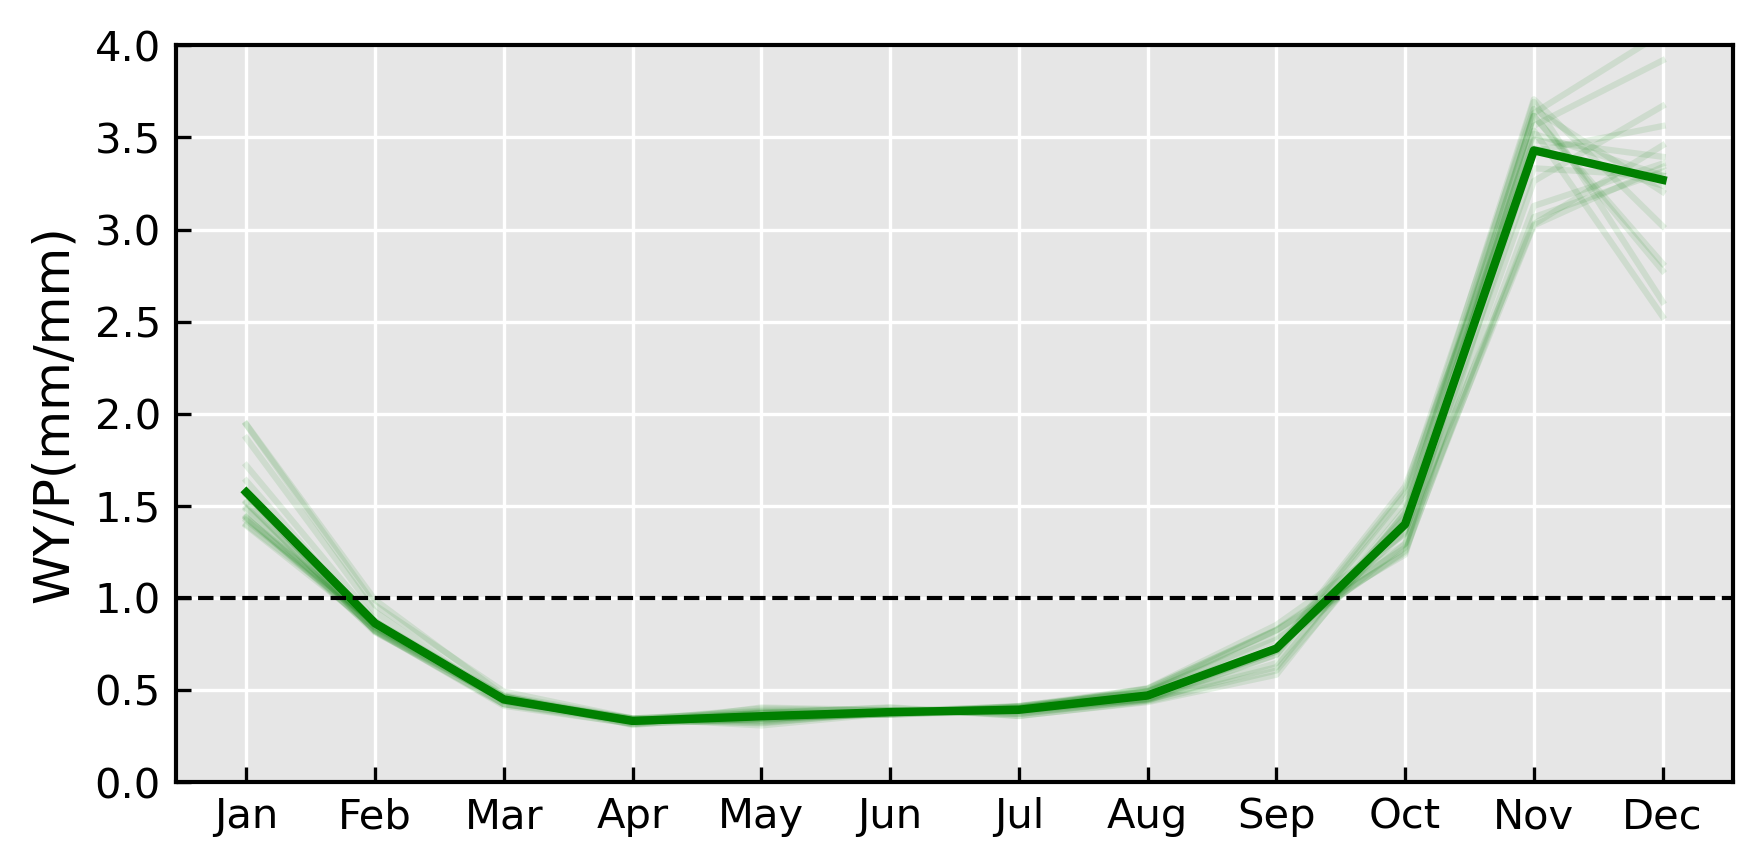
\includegraphics[width=12cm]{02-figures/runoff-ratio.png}
    \captionsetup{labelformat=empty}
    \caption{Figure R1. Monthly runoff-precipitation ratio observed in the Nuxia hydrological station. The green line represents multi-year average value and the light green lines represent the runoff-precipitation ratio from 1982 to 2013 (32 years).}
\end{figure*}

\point{Section 2.2: 
What is the temporal resolution of runoff, climate and vegetation data? 
In addition, please add in this section information about how the extensions of glacier and snow-covered areas were obtained.
Furthermore, I suggest reporting the time series of water yield for all catchments in the main manuscript to show the detected turning points.}
\reply{Thanks for your comments. In this study, we align the climate and vegetation data with runoff from 1982 to 2013. The description about the temporal resolution of climate and vegetation data used here has been incorporated into the revised version.}

\revised{70-73}{Here we collect annual runoff observations \ul{from 1982 to 2013} and convert the river flow ($m^{3}/s$) into runoff depth ($mm$). Also, we acquire high-resolution climate and vegetation data \ul{in the same time range}, and further aggregate these gridded data into regional annual values by considering area-weighted effects.}

\nextreply{Also, we reported the source of land use and cover used in our study in this section.}

\revised{93-95}{The land use and cover in 2000 with a spatial resolution of 1x1 km is used to represent the land cover types in the UBR basin. The data is acquired from Resource and Environmental Science Data Center, and is here divided into seven primary land use types, including cultivated land, forestland, grassland, water body, urban land, unused land, and glaciers and snow (Figure \ref{figS:lucc}).}

\nextreply{Finally, We have added the annual time-series of water yield for all catchments to show the detected turning points (see Figure \ref{figS:time series} in the supplementary), clearly illustrating a reversed or slowed WY changing direction but an increase of WY magnitude in the UBR basin (Figure \ref{fig:magnitude-direction}).}

\begin{figure*}[ht]
    \centering
    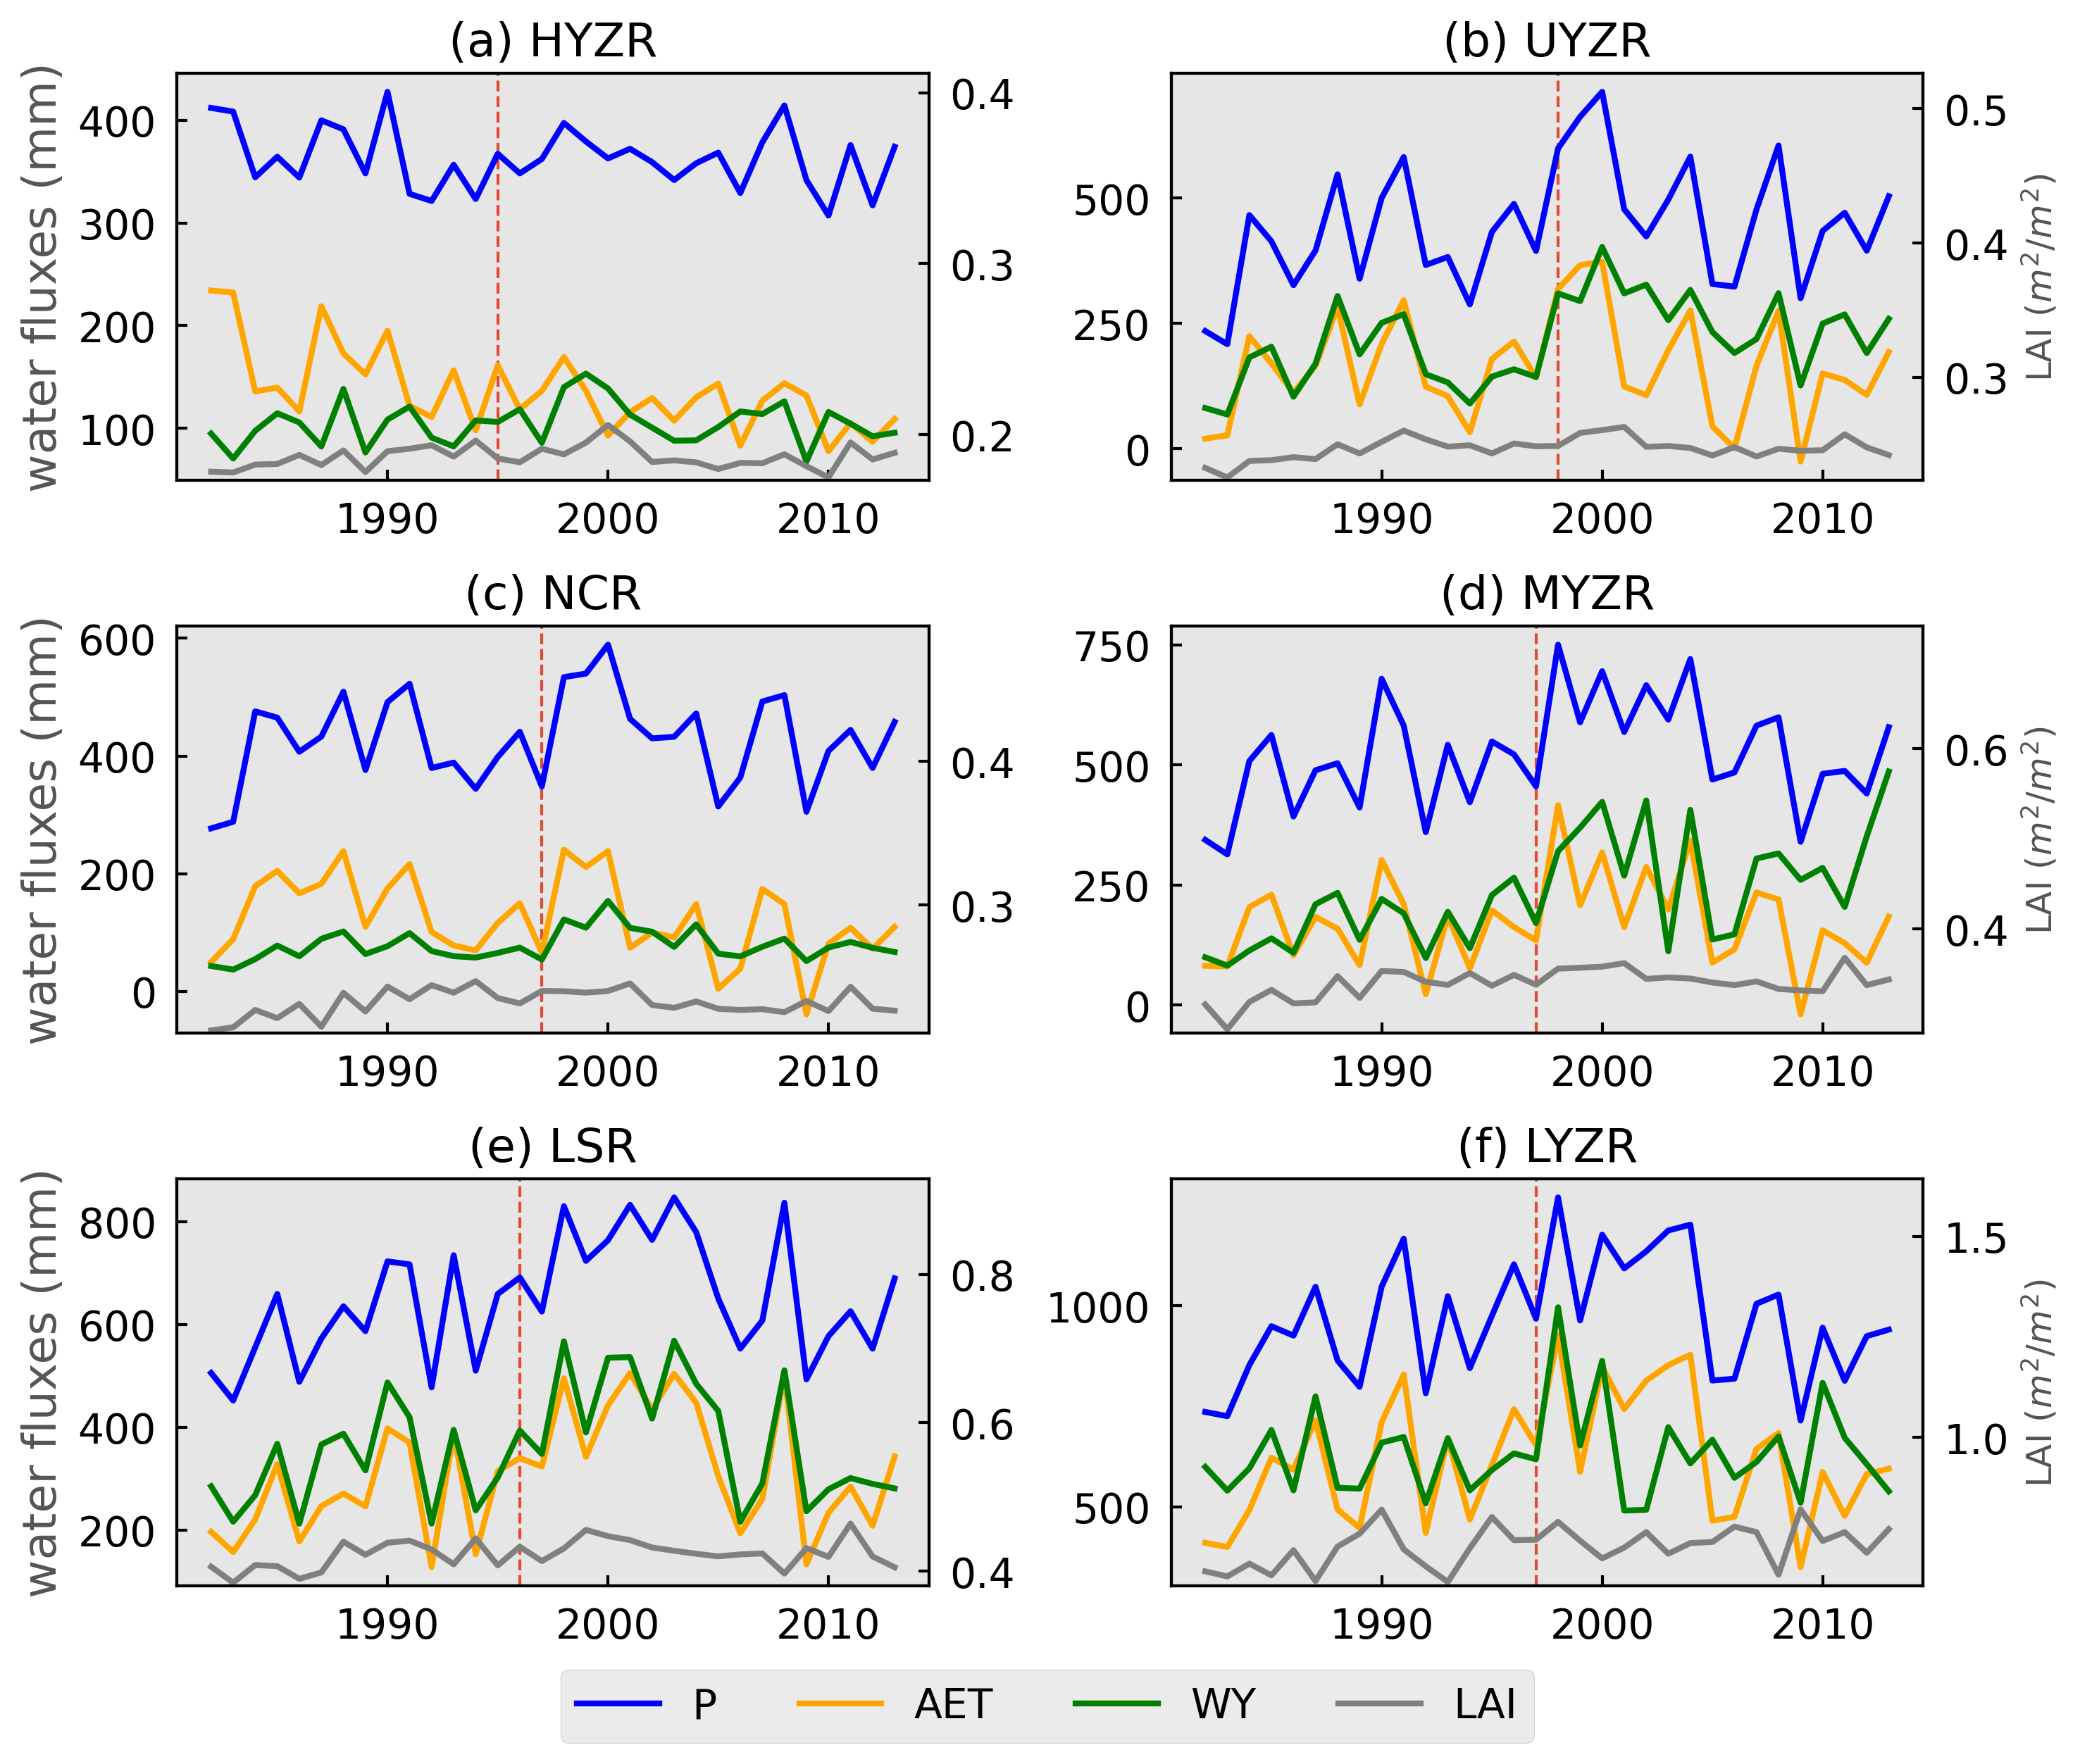
\includegraphics[width=12cm]{02-figures/time-series.png}
    \captionsetup{labelformat=empty}
    \caption{Figure \ref{figS:time series}. The temporal changes of precipitation (P, blue line), actual evaporation (AET, orange line), and water yield (WY, green line) and Leaf Area Index (LAI, grey line) during 1982--2013 in the entire UBR basin. The vertical line indicates the turning point in WY.}
\end{figure*}

\point{Section 2.3: As stated by the first reviewer, the methodological approach is unclear and difficult to understand. To improve the clarity of this section, I invite the authors to add an example of the double mass curve for one of the catchments, combined with a scheme that should help the reader to understand how the three components (climate, vegetation and cryosphere) were identified. For an example of what I mean, please see Figs. 2 and 3 in Brahney et al. (2017).}
\reply{Thanks for your suggestion. We have rewritten the method with the help of the schematic diagram (Figure \ref{fig:example_DMC}) for the DMC method in the main text (see Details in Methodology).}

\begin{figure*}[ht]
    \centering
    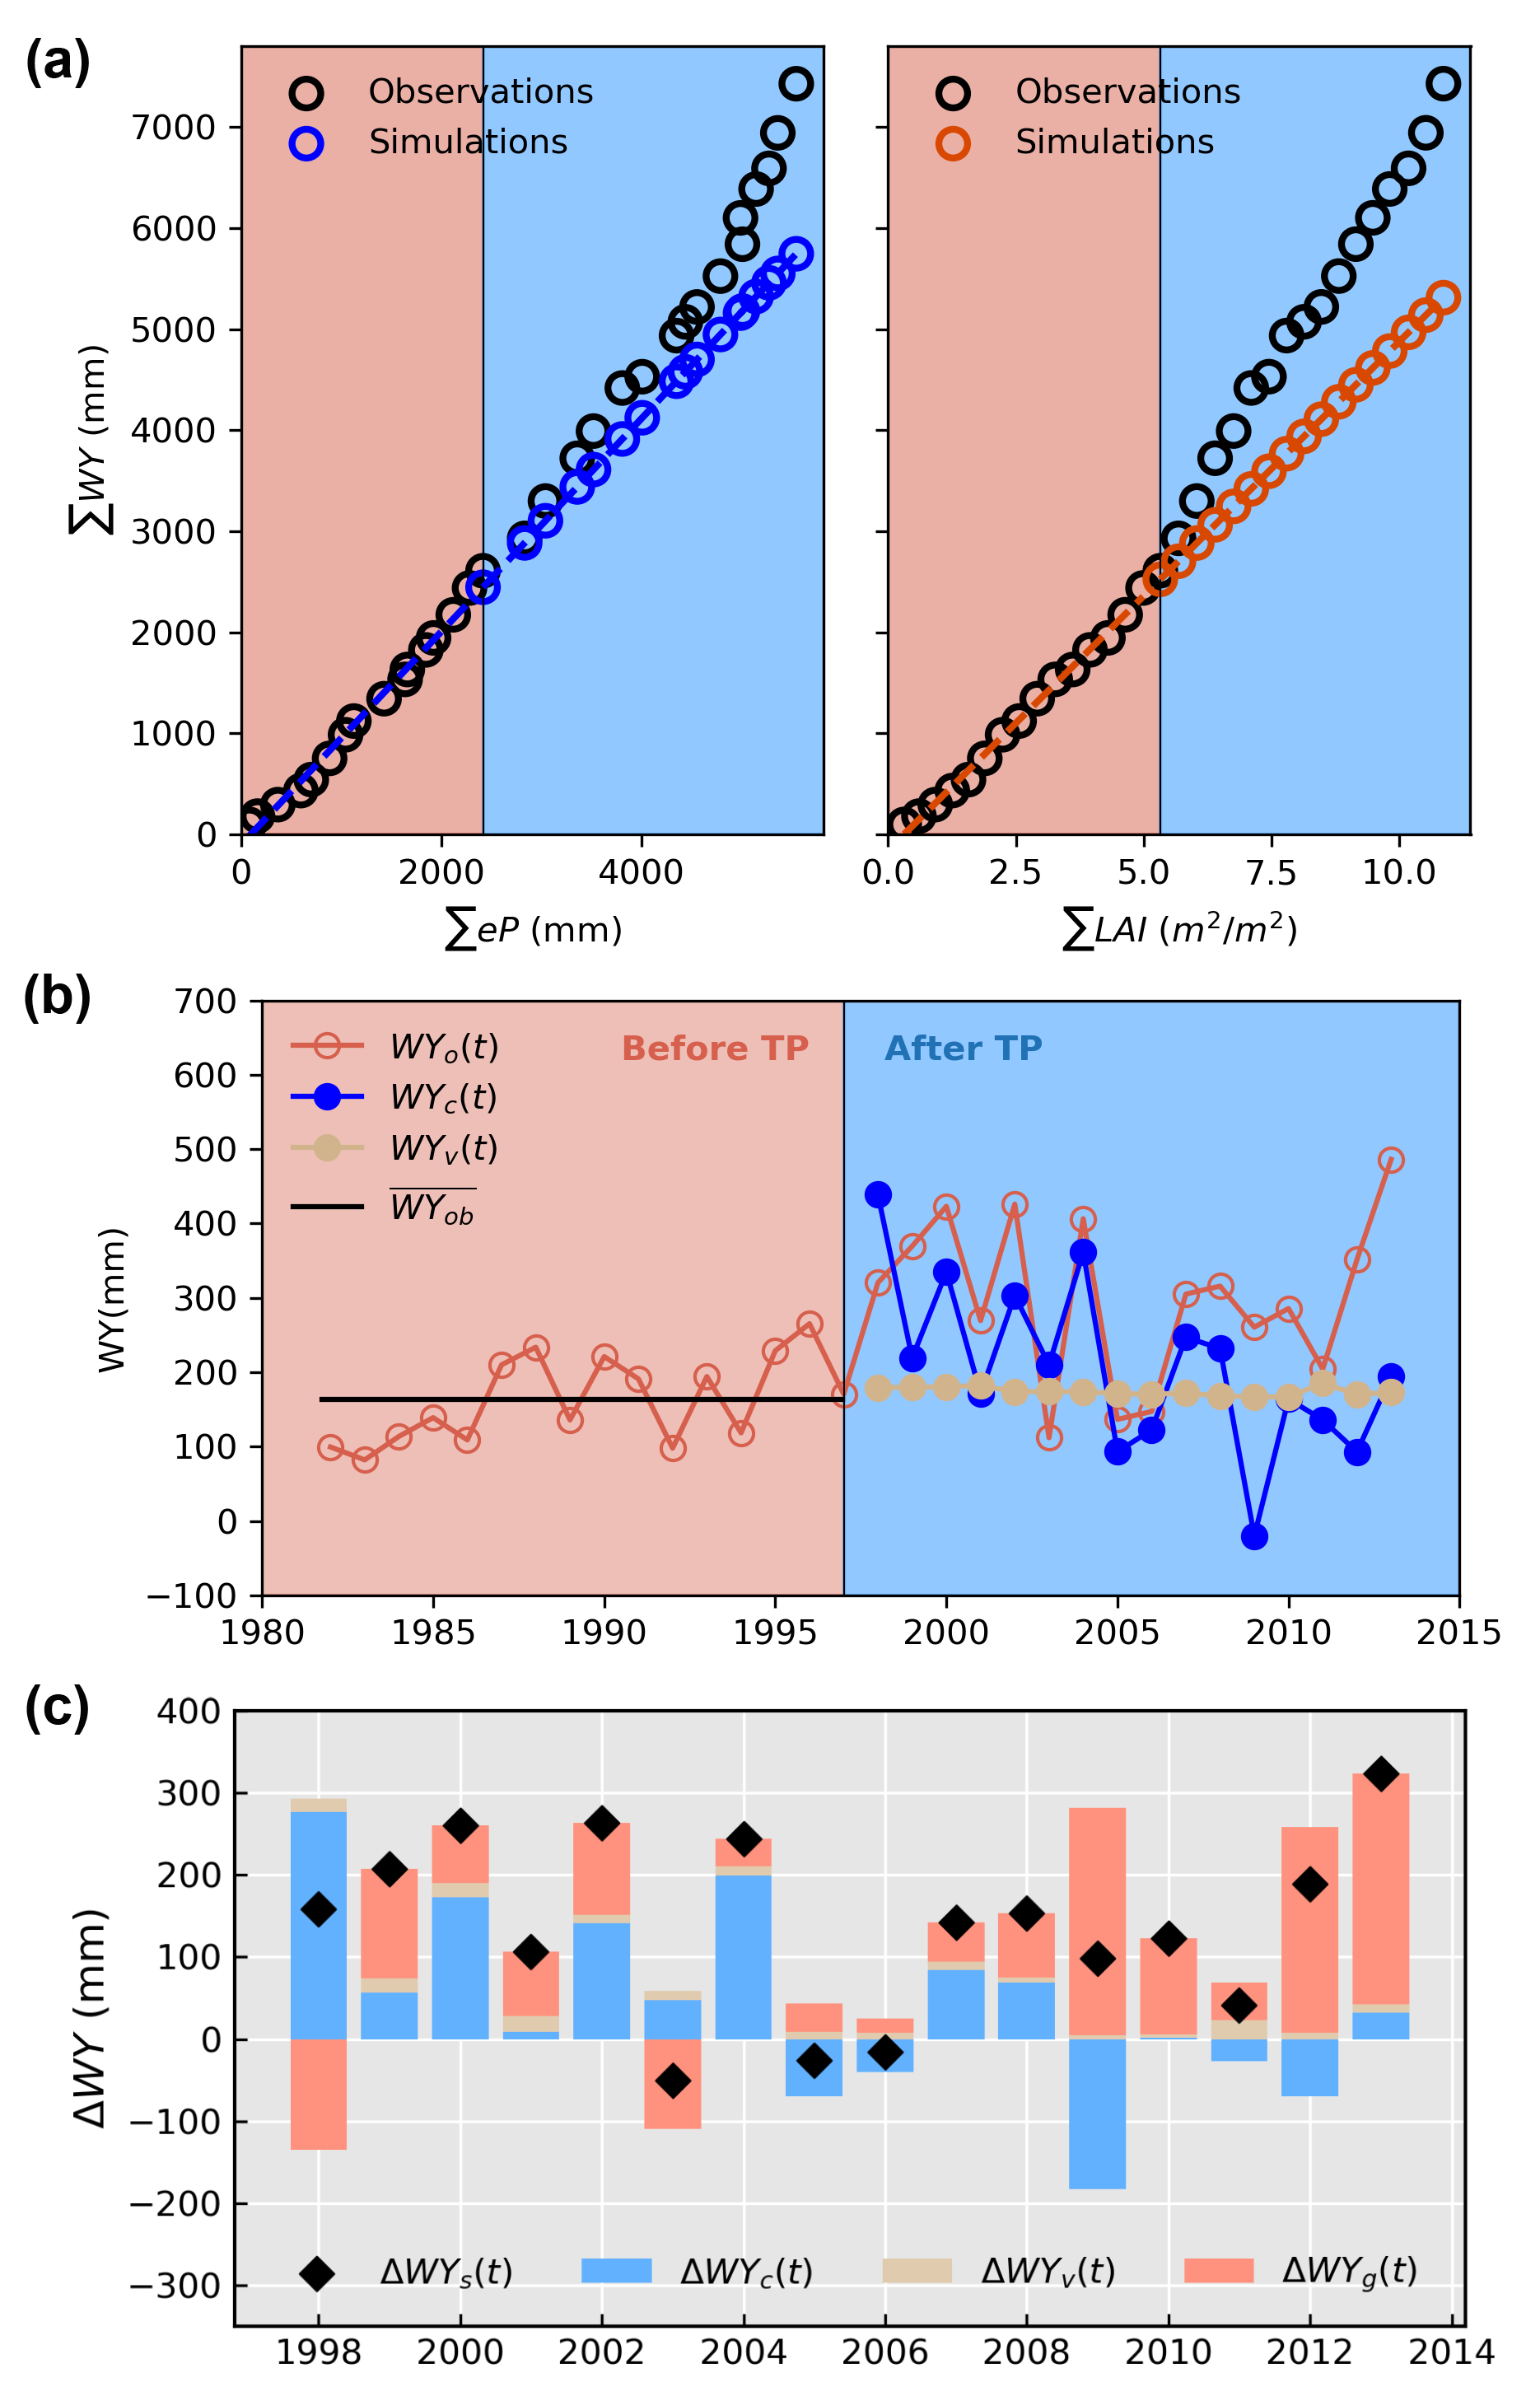
\includegraphics[width=9cm]{02-figures/example_DMC.png}
    \captionsetup{labelformat=empty}
    \caption
    {Figure \ref{fig:example_DMC}. The schematic diagram showing how to estimate the effects of climate, vegetation, and cryosphere on water yield in the MYZR basin (Details in Methodology).}
\end{figure*}

\point{Section 2.3.2: In this section it is unclear whether water yield and eP represent the same term (L155) or they were computed in a different way. Based on Section 2.2.1, water yield was obtained using only runoff data, whereas at L149-150, runoff is not mentioned as term of the water balance and for the computation of the water yield. Please rephrase all these sentences to clarify the definition of the two terms and their differences.}
\reply{We are sorry for this ambiguous description here. Here, water yield comes from observations in hydrological stations, while the effective precipitation (eP, P-AET) is calculated by the high-resolution datasets. In Line 149-150 in the original manuscript, we want to state the reasons why we want to use the eP (P-AET) rather than P or AET individually, because of the more direct connections between eP and water yield revealed by the water balance equation ($WY = P - AET + \Delta S$). Now, we have rephrased related texts to describe the selection of climate and vegetation index for building the DMC model in Line 111-117.}

\revised{112-118}{The selection of climate and vegetation indices used in the DMC technique is an important issue. Previous studies have shown that effective precipitation (eP, P-AET) can reflect more information of climate on WY compared with individual P or AET, and be regarded as a reliable proxy to climate \citep{wei2010quantifying,zhang2019separating}. LAI quantifies the amount of leaf area in an ecosystem and becomes an important variable reflecting vegetation structures and biophysical processes \citep{fang2019overview, forzieri2020increased}, and \citet{li2021vegetation} has used LAI to investigate vegetation effects on seasonal hydrology in the UBR basin. Hence, we consider eP and LAI as the indices of climate and vegetation respectively, and use their time series as the inputs in the DMC model.}

\point{L172: Did the authors take the sum of the mean annual LAI or did they compute the cumulative in a different way? How does LAI vary spatially and temporally in each catchment? Please add more details.}
\reply{We always use the cumulative LAI (or eP) as the explained variable and the cumulative WY as the response variable to build the double cumulative curve. The calculation of the cumulative values is the same for ep, LAI, and WY by taking the sum of the mean annual values. In the revised version, we provided a schematic diagram to show the DMC's procedure (Figure \ref{fig:example_DMC}).}

\nextreply{We also added the time-series of LAI in individual basins in the supplementary (Figure \ref{figS:time series})}

\point{In the results section, please remove all sentences referring to the discussion of the main findings.}
\reply{Thanks for your suggestions. We have removed them into discussion.}

\point{Section 4: I would like to see in this section also a discussion of the limitations of the approach used in this study. For instance, what is the uncertainty in precipitation, actual evapotranspiration and LAI in these catchments, and how do the uncertainties affect the main findings of this manuscript?}
\reply{Thanks for your suggestions. We have rewritten the discussion, including (1) uncertainties and limitations of the used data and DMC method used here, and (2) provided broad implications for mountainous water resource management.}

\nextreply{The limitations about the DMC model used in the study are presented in Line 234-248}

\revised{235-249}{This study has some limitations regarding the DMC model to partition the effects of climatic and cryospheric changes on the hydrological regime shifts in the UBR basin. 
The DMC method is a useful alternative statistical method to physical modeling approaches, especially in alpine river basins (e.g. UBR basin) where there is less knowledge on the complex hydrological mechanisms.
While the method is still dependent on our prior understanding of hydrological responses to warming and related environmental changes, such as glaciers melting and vegetation greening. 
For the UBR basin, besides climate change, cryosphere \citep{biemans2019importance,yao2019recent} and vegetation \citep{li2021vegetation,li2019greening} are two major factors for hydrological changes, and the cryospheric contributions can be regarded as the deviations between total water yield and climate and vegetation contributions estimated by the DMC method.
While, in some mountainous basins, human activities, such as urbanization, dam regulation and irrigation, may consume severely water resource or change seasonal runoff patterns, and thus we have to consider anthropogenic impacts into the DMC statistical model for river flow attribution. 
On the other hand, the DMC method applies the linear assumption between two variables, and thus it may fail to capture some nonlinear process among the interactions among water yield, vegetation and cryospheric melting in the study. Thus, with the availability of long-term in-situ observations and high-resolution remote sensing datasets in the UBR basin \citep{wang2022observing}, other powerful statistical models considering nonlinear and casual structures should be applied to identify the causes of water yield changes \citep{runge2019inferring}}

\nextreply{The uncertainties about the data used in the study are presented in Line 249-262}

\revised{250-263}{The data used in the study may also give rise to some uncertainties for our results. 
The 10x10 km precipitation product used here is generated by topographical and linear corrections based on observations. As \citet{sun2020precipitation} pointed, while, the results of the linear correction approach highly vary with the station density. For example, the increased numbers from 4 to 10 stations in the basin will decrease the mean annual precipitation by about 20 mm. Hence, the reconstruction of precipitation dataset will rely on the density of the observed stations. 
Besides the topographic correction, the effects of the basin size and climate seasonality should be considered in the work of precipitation reconstruction in the UBR basin due to the complex climate and environment \citep{sun2019contrasting}. 
Compared with precipitation, the estimation of evaporation may be much more challenging in high mountains. Although GLEAM actual evaporation shows the good agreement with in-situ eddy covariance records \citep{yang2017multi}, its model structure does not include wind speed and solar radiation, which may affect the estimation of sublimation, and thus total evaporation \citep{li2019evapotranspiration}. 
In addition, the coarse spatial resolution with a 0.25$^{\circ}$ spatial resolution in GLEAM may be insufficient to estimate regional evaporation in the UBR basin. 
However, with the help of the Second Tibetan Plateau Scientific Expedition and Research, the observation networks in meteorology, cryosphere and hydrology will be built, which is expected to benefit reliable precipitation and evaporation estimation, and make developing physically-based cryosphere-hydrological modeling possible \citep{wang2022observing}}

\nextreply{The implications of this study are presented in Line 264-274}

\revised{264-274}{Understanding the hydrological regime shifts and their causes in the high mountains are especially important in managing water resources, especially balancing the co-benefits between mountains and downstream lowlands \citep{viviroli2011climate}. 
In the study, the combined (offsetting or additive) effects from climate and cryosphere are detected (Figure \ref{fig:attribution-magnitude}), and further lead to either slight or substantial increases in WY in the entire UBR basin (Figure \ref{fig:magnitude-direction}a). 
The combined effects often hinder the roles of each driver in hydrological changes \citep{wei2018,zhang2021deforestation}, which should be considered when designing water management strategies in the large transboundary river system.
For example, the additive effect may be beneficial for mitigating droughts and water shortage during droughts, but it may exacerbate the flood risks due to increased precipitation and accelerated melting of the cryosphere in the future \citep{Immerzeel2013}.
In addition, our results clearly show that the melt waters from glaciers might have already surpassed the "peak water", and the associated hydrological changes will substantially affect future water resources management. Thus, the projections of the occurrence time of "peak water" will be important in managing mountainous water resources.}

\point{Fig. 1: In (a) it is difficult to identify the dots. In (b), the dots are small and partially hidden by the labels, whereas in (c) the labels of the histogram are too small. Furthermore, the terms ‘unused land’ and ‘beach land’ are unclear.}
\reply{Thanks for your suggestions. We use the red point to indicate the hydrological stations in Figure \ref{fig:location}a, and adjust the location of labels in Figure \ref{fig:location}b. In addition, we placed the Figure 1c in the original manuscript into the supplementary (Figure \ref{figS:lucc}), and added the percentage of snow and glaciers in Table \ref{tab: table 1} in the main text in the revised version.}

\nextreply{We are so sorry for showing land cover classification in the second level, and now we only show the classification in the first level. That is, land cover includes cultivated land, forestland, grassland, water body, urban land, unused land, and glaciers and snow (see Figure \ref{figS:lucc}).}

\begin{figure*}[ht]
    \centering
    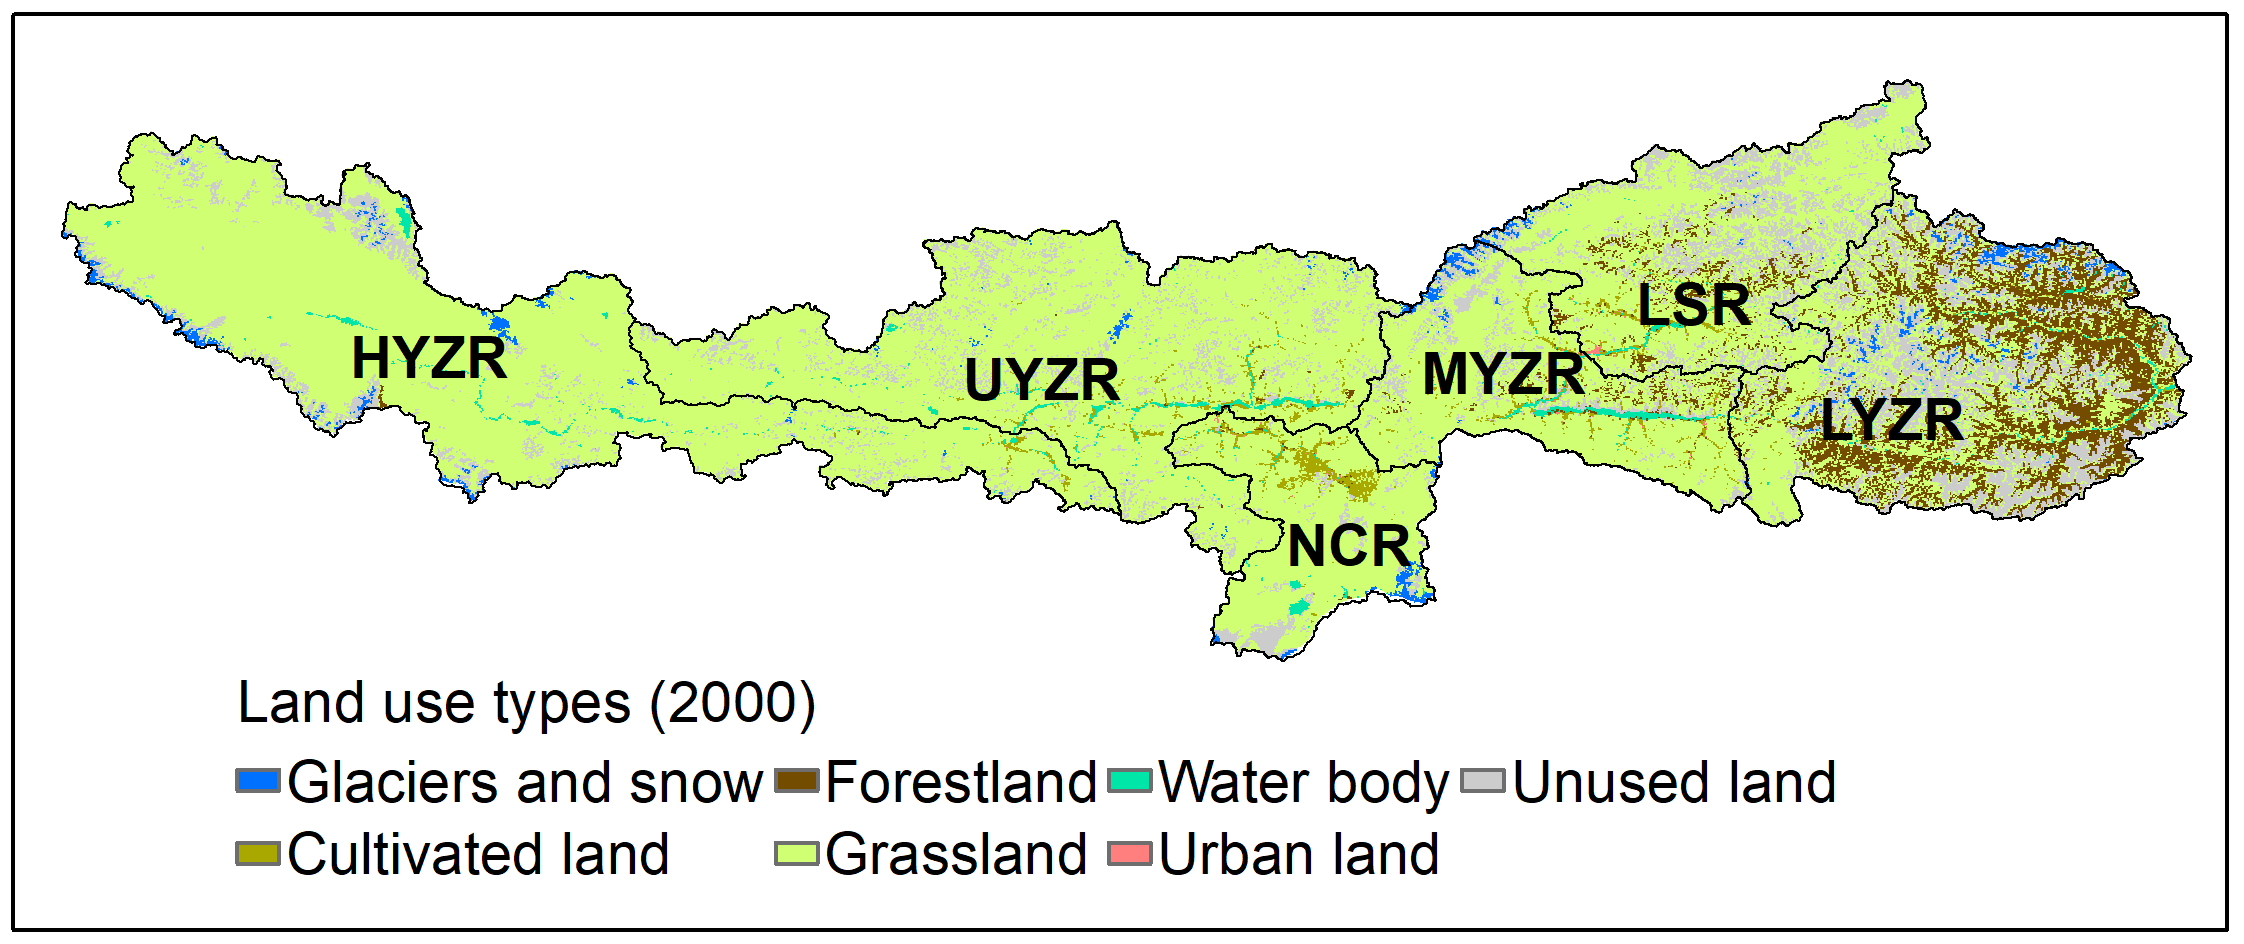
\includegraphics[width=8cm]{02-figures/lucc2000.png}
    \captionsetup{labelformat=empty}
    \caption{Figure \ref{figS:lucc}. The land use types in 2000 in the UBR basin.}
\end{figure*}

\nextreply{In addition, the "unused land" in land cover classifications means "Those ecosystems in which less than one third of the area has vegetation or other cover". In general, Barren Land has thin soil, sand, or rocks. Barren lands include deserts, dry salt flats, beaches, sand dunes, exposed rock, strip mines, quaries, and gravel pits" (\url{https://www.hq.nasa.gov/iwgsdi/Barren_Land.html})}

\begin{figure*}[ht]
    \centering
    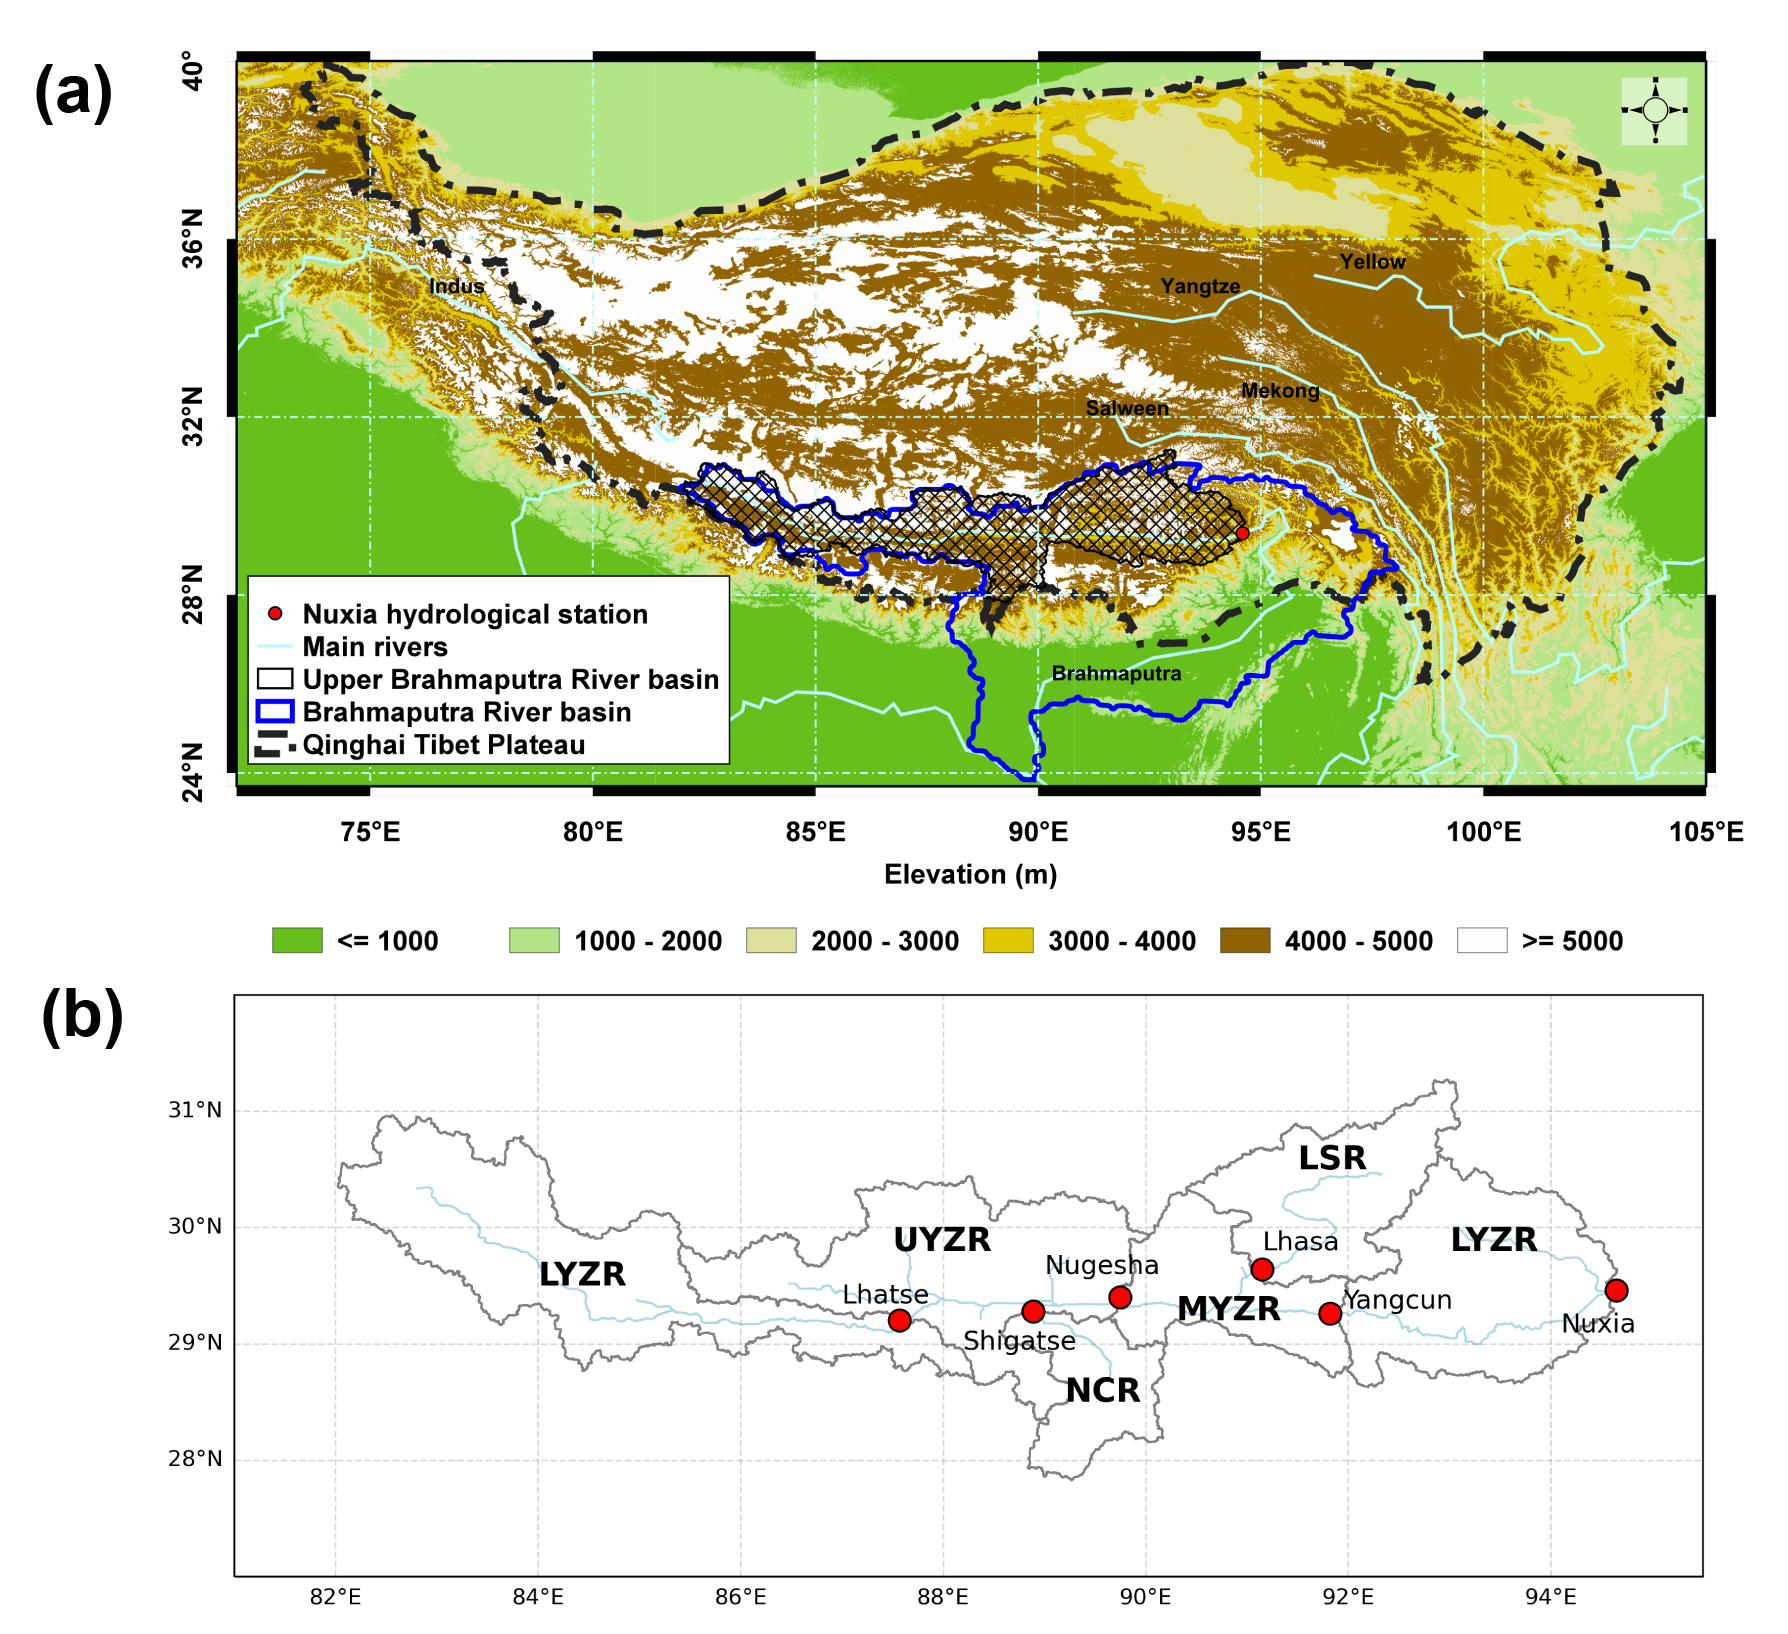
\includegraphics[width=8cm]{02-figures/Figure1.png}
    \captionsetup{labelformat=empty}
    \caption{Figure \ref{fig:location}. Location of (a) the Upper Brahmaputra River (UBR) basin in the Qinghai Tibet Plateau (QTP), which is from \citet{li2021vegetation}, and (b) six basins divided by Lhatse, Nugesha, Shigatse, Yangcun, Lhasa, and Nuxia hydrological stations.}
\end{figure*}

\point{Fig. 5 in the main manuscript and Fig. 6 in the response to the reviewers: Some grey/light brown regression lines seem very flat, but still the correlation coefficients are $>$0.5 and significant. Please check whether there are mistakes in the statistical analyses.}
\reply{Thanks for your questions. We have checked the results and they are correct. Vegetation-induced water yield (tan points) is much weaker compared with those caused by climate and cryosphere, and hence the fitted line is significant but looks flattened when we showed all the data in each panel. To avoid some misunderstandings, we have labelled the Pearson's correlation coefficients and shown the regression line only when the correlation is significant (p $<$ 0.05) in Figure \ref{fig:attribution-direction} in the revised manuscript. In addition, we also take the UYZR basin as an example to only show vegetation contributions and water yield deviations here (Figure R2).}

\begin{figure*}[ht]
    \centering
    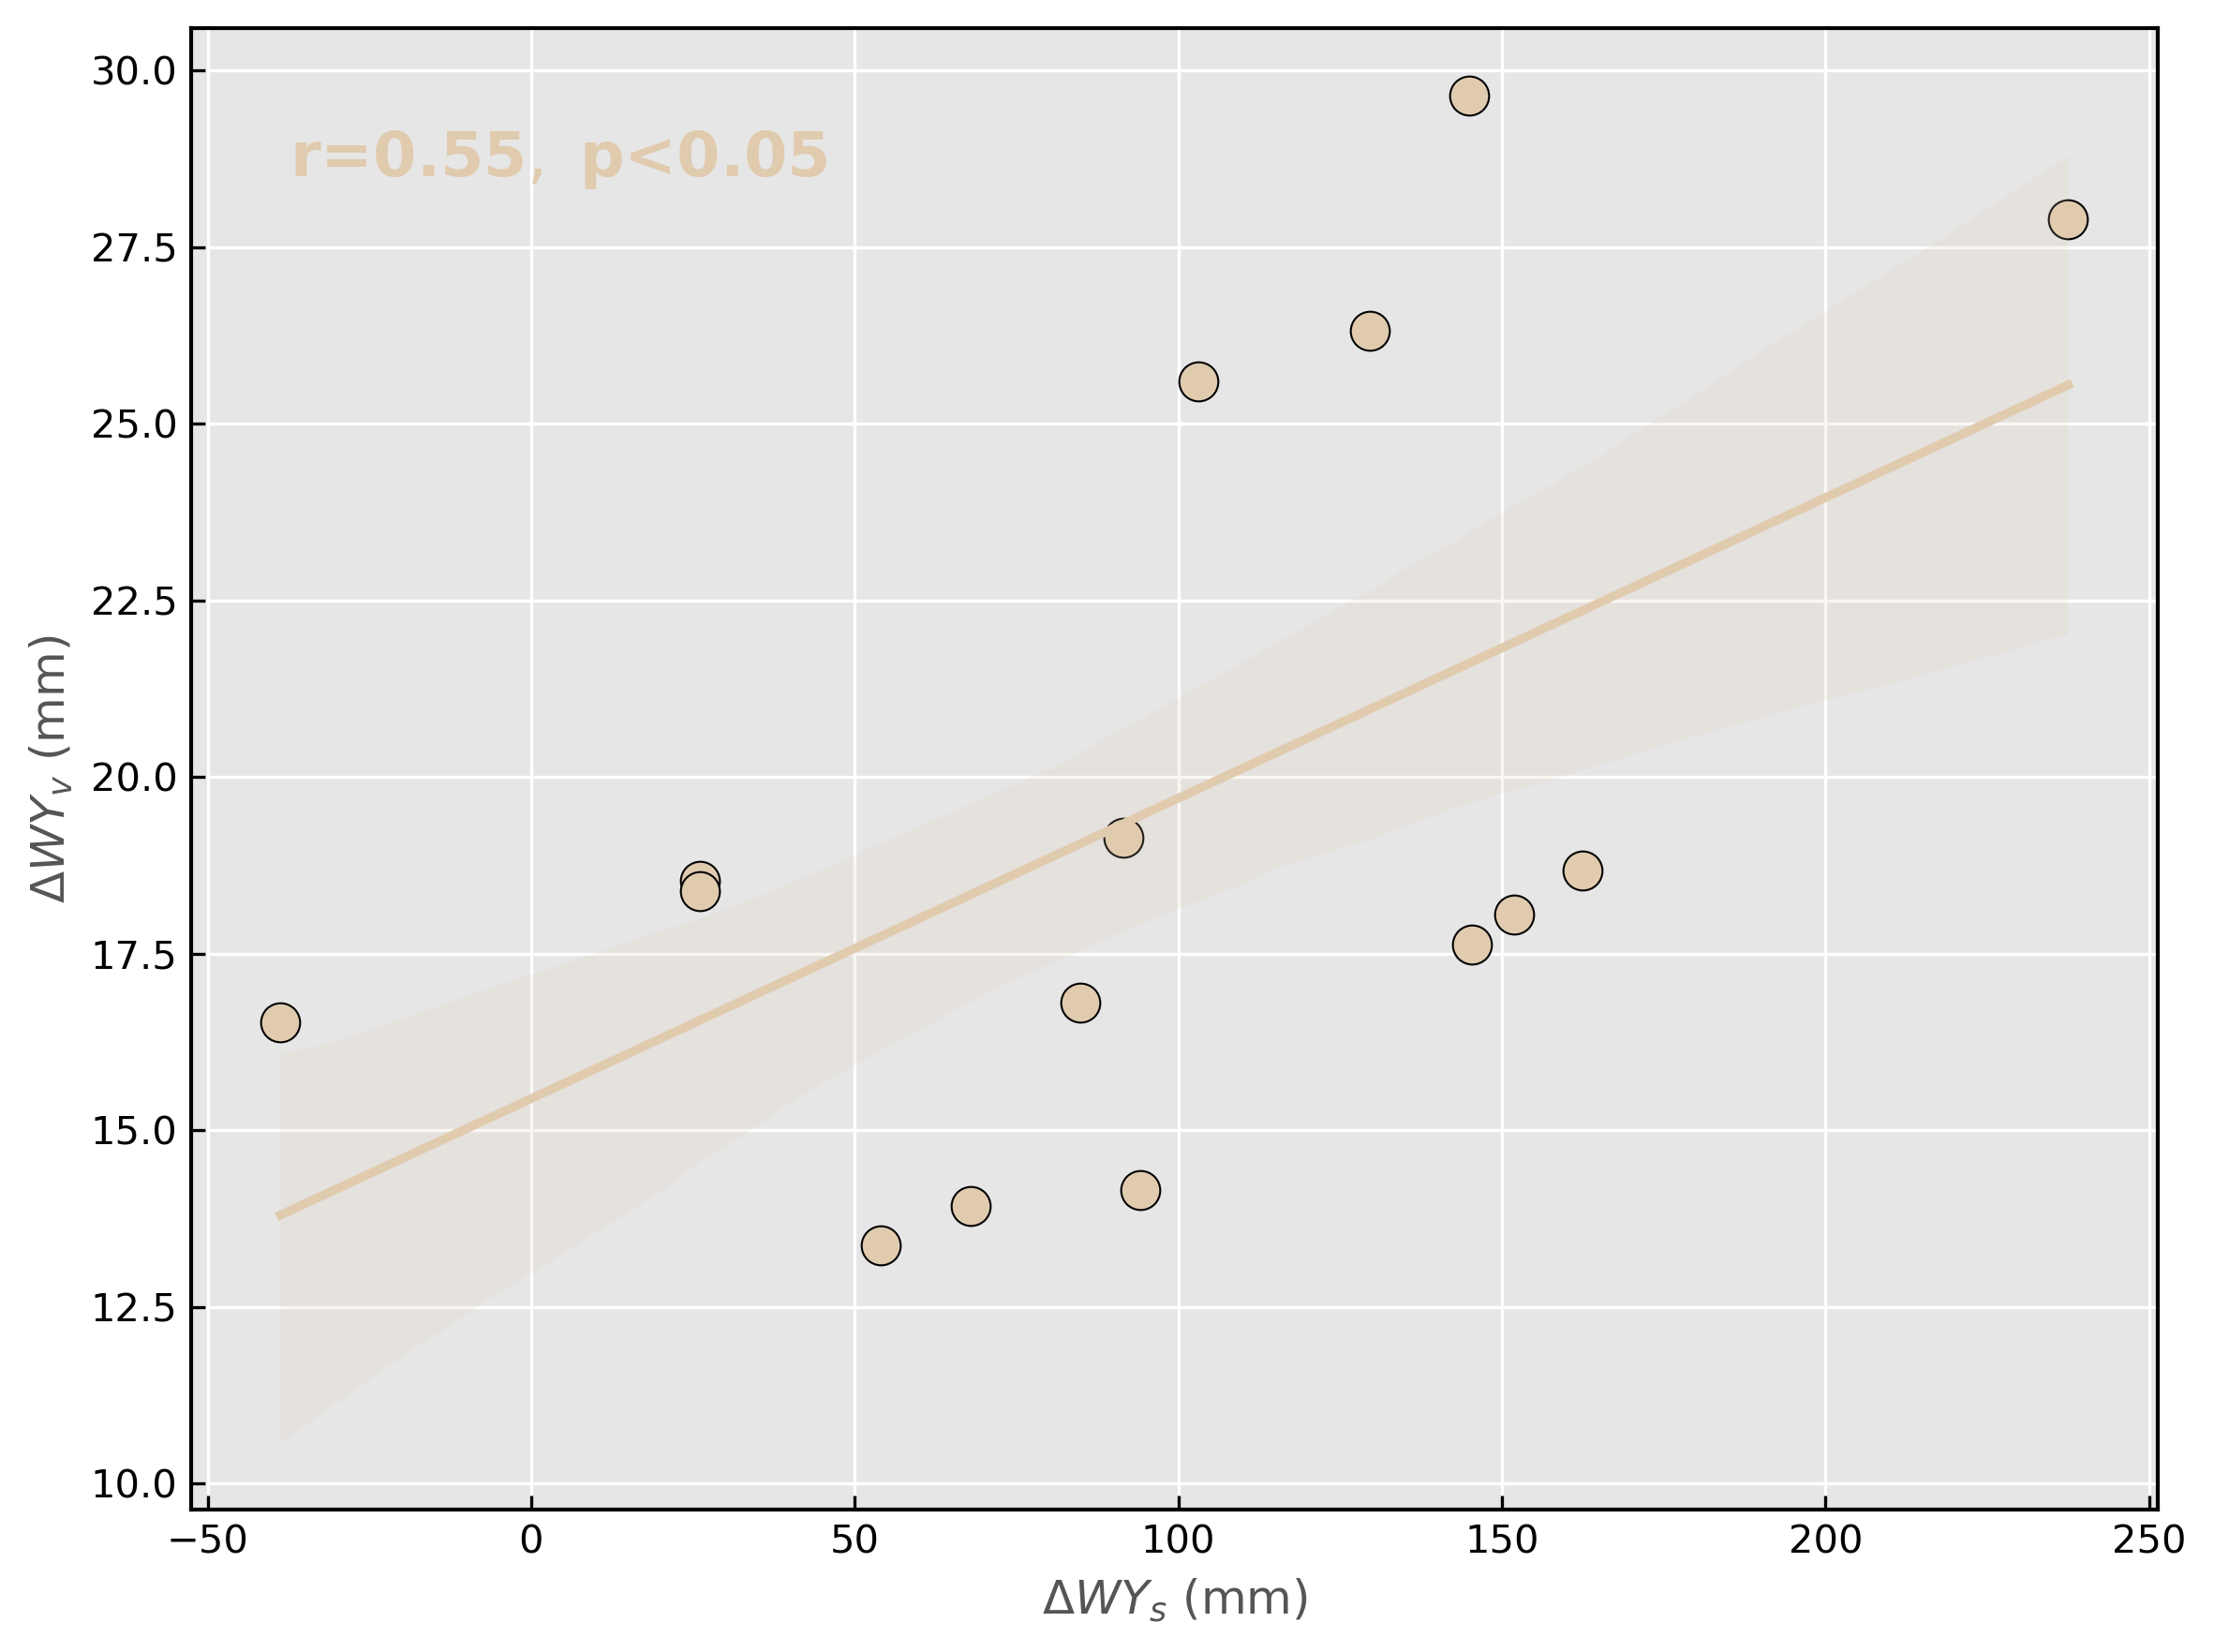
\includegraphics[width=6cm]{02-figures/corr-LAI-WY.png}
    \captionsetup{labelformat=empty}
    \caption{Figure R2. The scatter plot between vegetation contributions ($\Delta WY_v$) and total water yield deviations ($\Delta WY_s$) in the UYZR basin.}
\end{figure*}

\point{Table S2: Some turning points are not significant. Based on these results, DMC analyses should not be performed for those catchments where the turning points were not significant.}
\reply{Thanks for your question. As you pointed, the Pettitt method does not find the significant abruption in some watersheds (Table \ref{tab: table 1}), which potentially indicates the divergent causes for hydrological changes in the UBR basin and the significance of comprehensive assessment on water yield responses to climate warming.}

\nextreply{Although some watersheds don't have significant turning points, we still find hydrological regime shifts in these regions (Figure \ref{fig:magnitude-direction}). For example, for the HYZR basin with non-significant turning point in 1995, water yield increased by $\sim$10\%, and its changing direction is reversed from increasing to decreasing. The hydrological regime shifts in the entire UBR basin, including magnitude and direction, fuel our interest to find potential causes.}

%%%%%%%%%%%%%%%%%%%%%%%%%%%%%%%%%%%%%%%%%%
%%%%%%%%%%%%%%%%%%%%%%%%%%%%%%%%%%%%%%%%%%
\reviewersection
%%%%%%%%%%%%%%%%%%%%%%%%%%%%%%%%%%%%%%%%%%
%%%%%%%%%%%%%%%%%%%%%%%%%%%%%%%%%%%%%%%%%%

\point{Li et al. provide a case study to study the influence of climate and cryosphere on the water yield in the Brahmaputra. To do this they collected a long time series for climatic and precipitation data and analyzed it to find the water yield has changed over the time period studied.
They find that there are substantial changes and attribute this mainly to the combined effect of climate and cryosphere. I think this study has value (I especially like the introduction) and should be considered for publication. However, I have several issues that I think should be addressed.}
\reply{We are grateful for Dr. Florian Ulrich Jehn's thoughtful evaluation and support of our work. We will reply to comments in the following, including \textbf{(1) clarifying the reasons for selections of climate and vegetation indices}, and \textbf{(2) providing a schematic diagram showing the procedure of the double mass curve (DMC)}.} 

\sect{General Comments}

\point{First, the study does not provide enough information about its data. 
For example, after reading the study I am still unsure what exactly is meant when the study talks about climate being a major factor in its analysis. Is it the mean temperature? Is it some indices? Is it something completely different? 
Same goes for the term cryosphere, which is used quite loosely.}
\reply{We thank the reviewer for pointing this out. We now clearly define (1) the effective precipitation (eP, P-AET) as a proxy to assess climate effects on water yield, and (2) meltwaters from glaciers and snow under warming as the cryospheric component in this study.}

\nextreply{Related definition about the selection of the climate indicator in the DMC is shown:}

\revised{112--114}{The selection of climate and vegetation indices used in the DMC technique is an important issue.
Previous studies have shown that effective precipitation (eP, P-AET) can reflect more information of climate on WY compared with individual P or AET, and be regarded as a reliable proxy to climate \citep{wei2010quantifying,zhang2019separating}.}

\nextreply{Related definition about meltwaters is shown:}

\revised{106-108}{For the large and pristine UBR and other mountainous basins, climate, vegetation, and \textbf{cryosphere (melt waters from glaciers and snow under warming, see \citealt{biemans2019importance,huss2018global})} play important roles in hydrology, and these three parts must be together considered to accurately estimate hydrological responses to warming.}

\revised{119--121}{To obtain cryospheric contributions to WY, we firstly build two types of DMC plots (see Figure \ref{figS:DMC}) to assess the contributions of climate (eP) and vegetation (LAI), and then subtract the sum of estimated contributions from total WY deviations as cryospheric effects (results are shown in Figure \ref{fig:attribution-results}). The schematic diagram \ref{fig:example_DMC} and associated mathematical formulas are shown as follows: ...}

\point{Second, after reading the methods it is not clear to me how the study is able to differentiate between the influence on climate, cryosphere and vegetation. This section would profit from a more in depth explanation.
In addition, why using this method?
Why do you think it is especially good for your kind of study?}
\reply{We thank the reviewer for this question. In the revised version, we provide the detailed reasons and a schematic diagram (Figure \ref{fig:example_DMC}) to show why and how we use the DMC in the study.}

\begin{figure*}[ht]
    \centering
    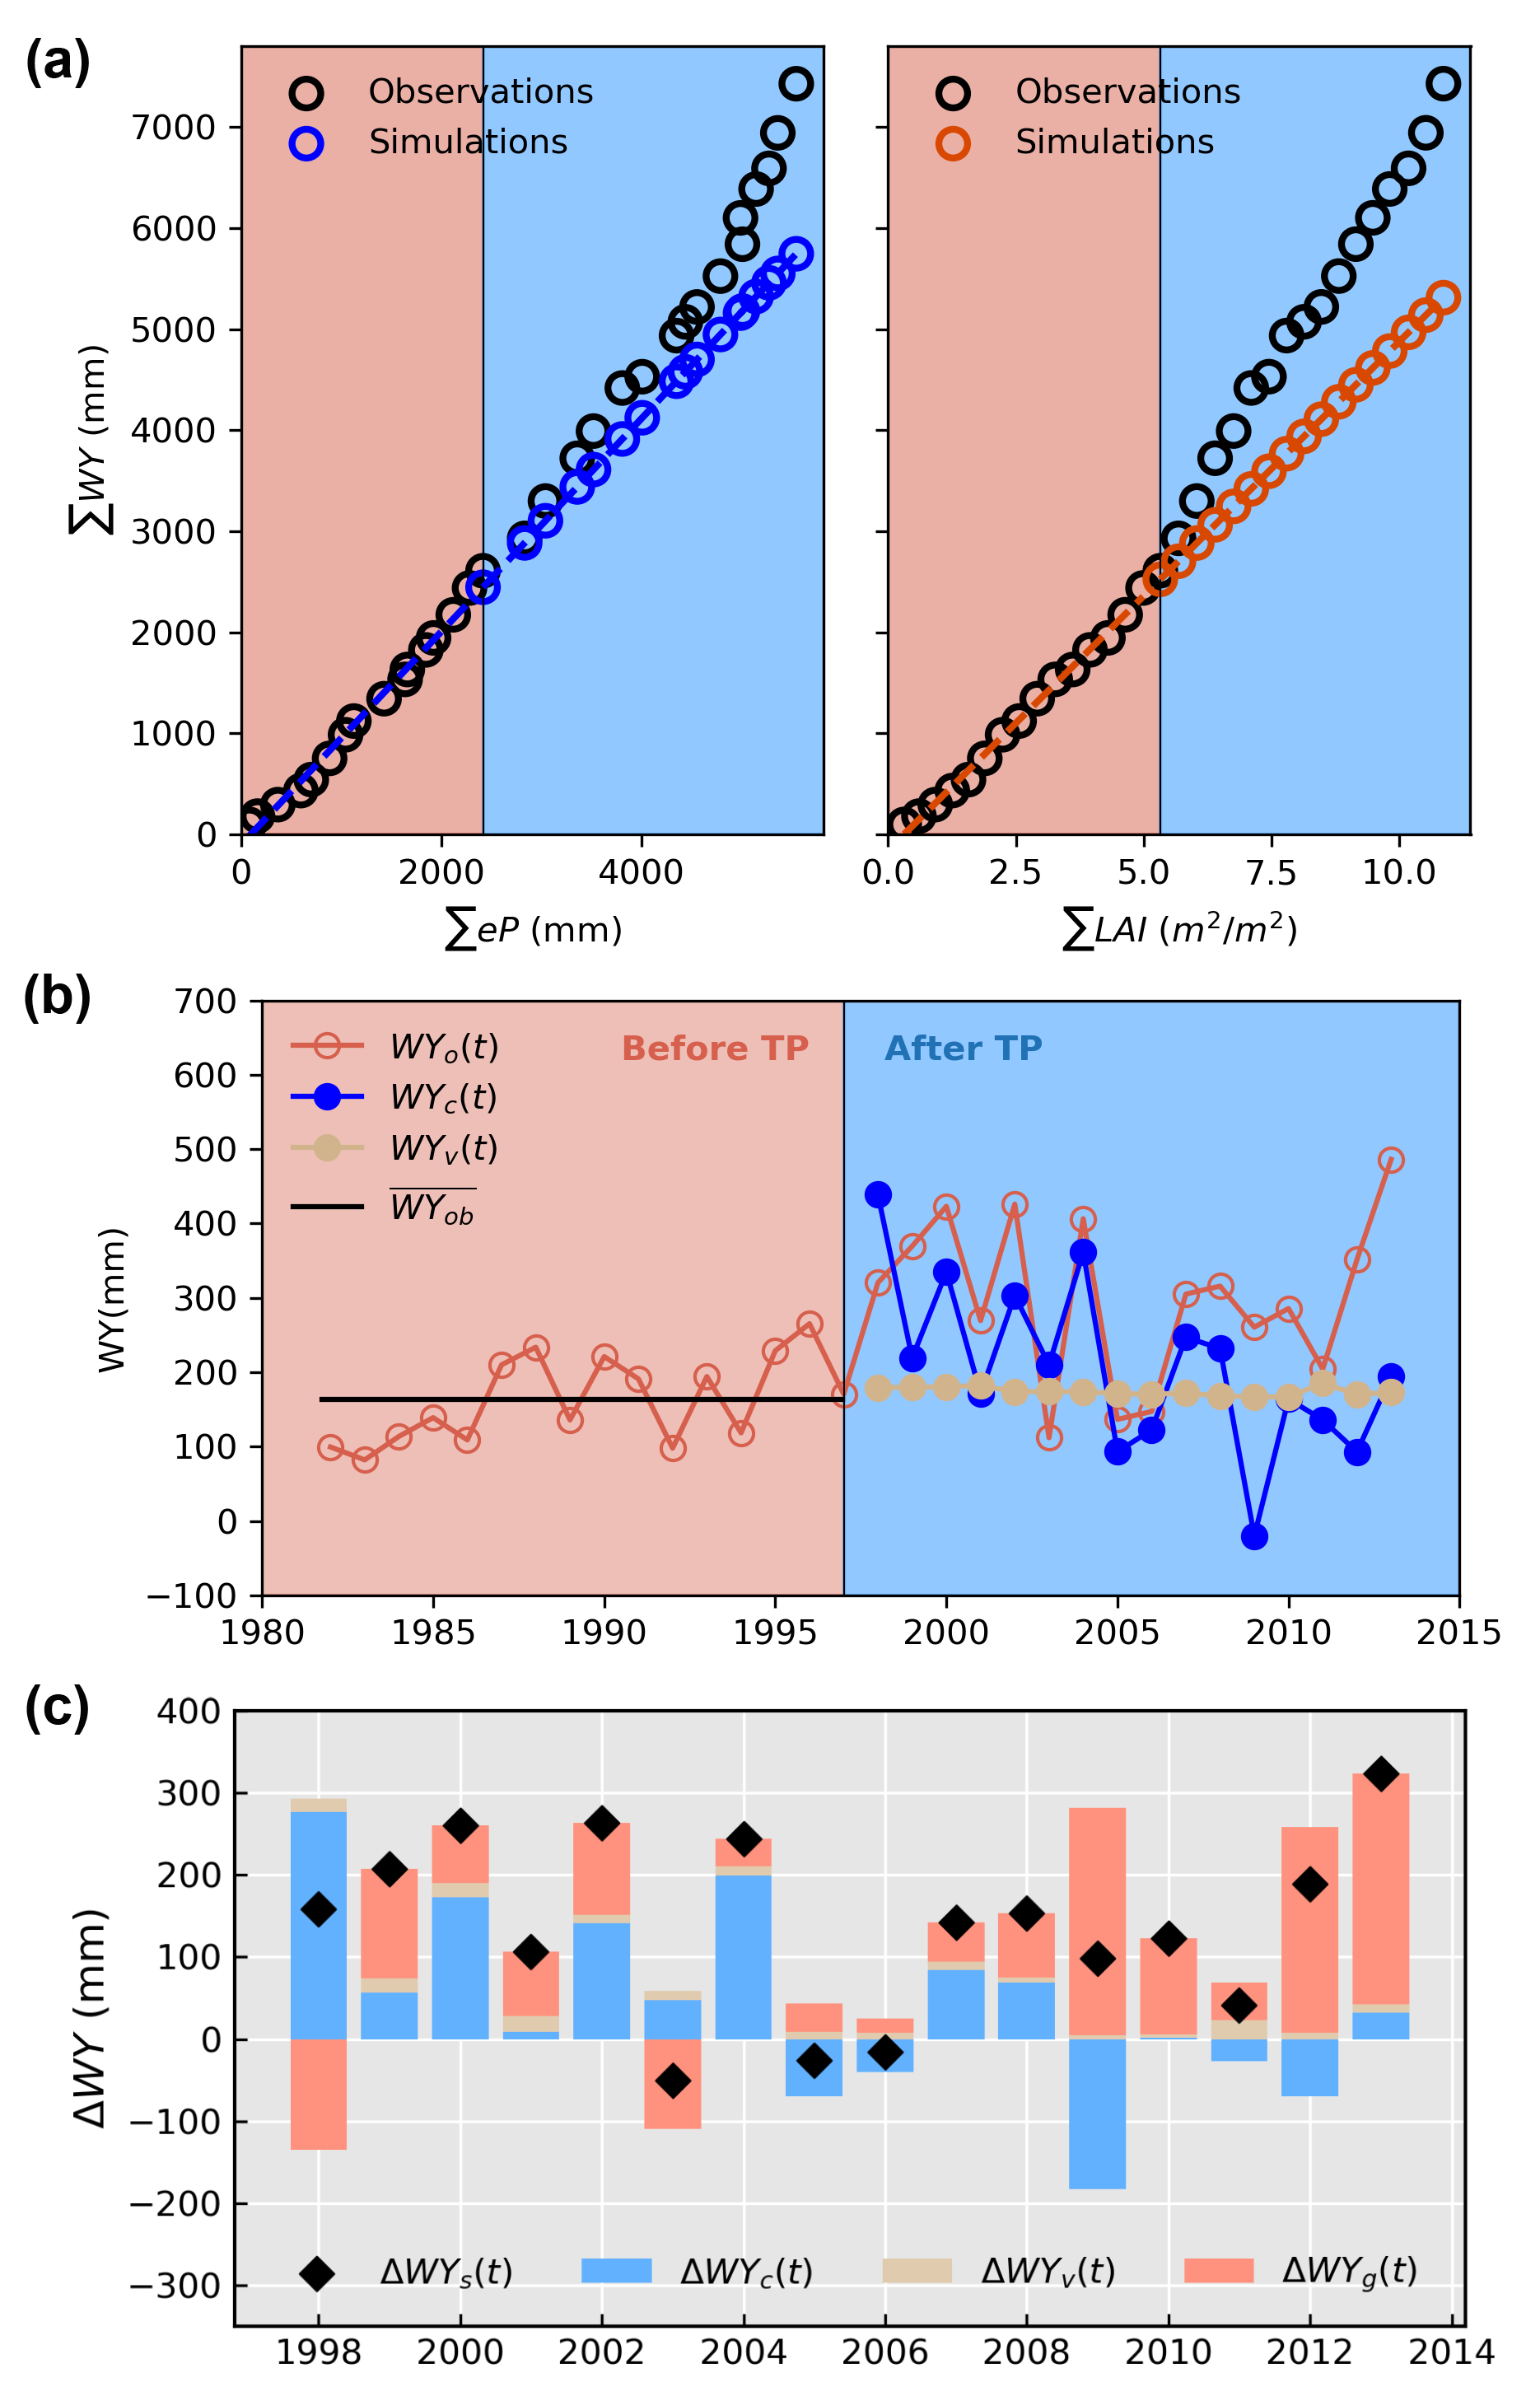
\includegraphics[width=9cm]{02-figures/example_DMC.png}
    \captionsetup{labelformat=empty}
    \caption
    {Figure \ref{fig:example_DMC}. The schematic diagram showing how to estimate the effects of climate, vegetation, and cryosphere on water yield in the MYZR basin (Details in Methodology).}
\end{figure*}

\nextreply{For a large natural mountainous watershed, it still remains not clear about the hydrological responses to climate change and associated environmental changes, e.g. vegetation and cryosphere. That leads to great uncertainties when assessing water yield changes using hydrological models. While, long-term annual runoff observations and high-resolution precipitation records in the UBR basin provide a good opportunity for statistical models to investigate hydrological responses to climate warming. The Double Mass Curve -- a data-driven statistical model -- has been widely been applied to estimate water yield responses to environmental changes in the hydrological community.
We assume that in the UBR basin, water yield is affected by climate (e.g. precipitation and evaporation), vegetation greening or browning, and cryospheric loss (e.g. glaciers and snow melting). Hence, we can estimate cryospheric contributions to water yield by subtracting the sum of contributions from climate and vegetation from total deviations using the DMC method. Related revisions are shown.}

\revised{46--49}{... Lastly, the present inadequate understanding of hydrological responses to complex interactions among climate, vegetation, and cryosphere limits the application of hydrological models in those glacier-fed watersheds \citep{pellicciotti2012challenges}. While, long-term observed runoff data and recent high-resolution precipitation records may give a pathway for using statistical methods to estimate runoff responses to warming in the UBR basin.}

\revised{103-111}{The DMC used here is a plot of the cumulative data of one variable versus the cumulative data of another related variable in a concurrent period.
It has previously been used to assess the individual effect of climate \citep{gao2011changes}, forest disturbance \citep{wei2010quantifying}, wildfire \citep{hallema2018burned}, and cryosphere \citep{brahney2017determining} on water resources.
For the large and pristine UBR and other mountainous basins, climate, vegetation, and \textbf{cryosphere (melt waters from glaciers and snow under warming, see \citealt{biemans2019importance,huss2018global})} play important roles in hydrology, and these three parts must be together considered to accurately estimate hydrological responses to warming.
It is considerably hard to directly calculate the supply of melt waters to WY due to the lack of long-term glacier monitoring, while runoff observations and high-resolution climate and vegetation data make it possible to use the DMC technique, a data-driven statistical method, to estimate cryospheric contributions to WY.}

\nextreply{In addition, with the help of the schematic diagram (Figure \ref{fig:example_DMC}), we now clearly explain the procedure for using the DMC to separate climate, vegetation and cryosphere contributions to water yield (see details in Methodology).}

\point{Third, the study finds a turning point for the behavior of the river. This seems quite important to me, but is never really discussed. Why did this change happen? What consequences will it have?}

\reply{We thank the reviewer for pointing this out, and have analyzed the causes of turning points and their implications in the revised manuscript.}

\nextreply{In this study, climate changes and meltwaters from glaciers and snow mainly contribute to substantial water yield changes before and after the turning point. 
Figure \ref{fig:attribution-magnitude} shows that the combined effects from climate and cryosphere contribute to magnitude increases in water yield, but Figure \ref{fig:attribution-direction} shows that climate is more important for the trend changes in water yield, while melt waters have the potential to mitigate water shortage risks. Related revisions are shown:}

\revised{180--183}{Climate and cryosphere -- two important factors affecting WY -- together contribute to \ul{over 80\% average magnitude increases} of WY in the entire UBR basin; however, they play both additive or offsetting roles (Figure \ref{fig:attribution-magnitude}), resulting in slight or substantial WY increases (Figure \ref{fig:magnitude-direction}a).}

\revised{190--193}{Results in Figure \ref{fig:attribution-direction} show that, although the correlation varies greatly across basins ranging from 0.11 to 0.93 after the TP, climate typically is positively associated with total WY, in which the correlation is significant in half of basins (p $<$ 0.05), again revealing \ul{the major role of climate} in the hydrological trends in the entire UBR basin.}

\revised{197--201}{In contrast to positive contributions of climate, we find that WY caused by cryosphere exhibits a negative association with reduced total WY deviations in recent years in the UYZR (r = -0.39, p $>$ 0.05) and LSR (r = -0.36, p $>$ 0.05) basins. 
The negative but weak relationship indicates that \ul{melt waters from cryospheric loss may compensate for low flow, and even mitigate water shortage risks}. 
Also, \ul{the compensating effect} from cryosphere is much stronger in the MYZR (r = 0.47, p $>$ 0.05), and together with climate contributions, contributes to the increasing WY trend (Figure \ref{fig:magnitude-direction}).}

\nextreply{Meanwhile, our results may suggest the occurrence time of "peak water" in the UBR basin, which is in line with \citet{huss2018global}, and we also add related analysis and discussion in the revised version.}

\revised{201--207}{Different from other regions, however, the HYZR basin shows a significantly positive relationship between cryospheric contributions and total WY deviations (r = 0.76, p $<$ 0.05), indicating that cryosphere instead of climate leads to the downward trend in headwaters.
This signifies that in this region, cryospheric contributions have already \ul{passed a maximum supplying to river flow}, due to decreased glaciers and snow under continuous warming.
The is further verified by the relationship of cryospheric contributions to total WY ($RC_g$) with temperature (Figure \ref{figS:warming-and-cryosphere}). 
In the HYZR basin, WY resulting from the cryosphere continues to increase with temperature until a maximum is reached, beyond which cryospheric contribution to total WY begins to decrease.}

\revised{227-233}{Cryospheric contribution is also important for water yield regime shifts -- melt waters from glaciers and snow melting can alleviate water resources shortages, mainly caused by decreased precipitation in recent years (Figure \ref{fig:attribution-direction}+\ref{figS:climate-directions}). This finding is also supported by observed glacier runoff data \citep{yao2010glacial} and several modeling studies \citep{lutz2014consistent, Zhang2020VariationOM, wang2021tp}. 
However, after glacier runoff reaches a maximum, defined as \ul{"peak water"} \citep{gleick2010peak}, cryospheric mass loss cannot sustain the rising melt waters with atmospheric warming (e.g. the HYZR basin in Figure \ref{figS:warming-and-cryosphere}), which is in agreement with \citet{huss2018global}.}

\nextreply{In the revised manuscript, we add the implications of our results on water resource management in mountainous watersheds.}

\revised{265--275}{Understanding the hydrological regime shifts and their causes in the high mountains are especially important in managing water resources, especially balancing the co-benefits between mountains and downstream lowlands \citep{viviroli2011climate}. 
In the study, the combined (offsetting or additive) effects from climate and cryosphere are detected (Figure \ref{fig:attribution-magnitude}), and further lead to either slight or substantial increases in WY in the entire UBR basin (Figure \ref{fig:magnitude-direction}a). 
The combined effects often hinder the roles of each driver in hydrological changes \citep{wei2018,zhang2021deforestation}, which should be considered when designing water management strategies in the large transboundary river system.
For example, the additive effect may be beneficial for mitigating droughts and water shortage during droughts, but it may exacerbate the flood risks due to increased precipitation and accelerated melting of the cryosphere in the future \citep{Immerzeel2013}.
In addition, our results clearly show that the melt waters from glaciers might have already surpassed the "peak water"  (Figure \ref{figS:warming-and-cryosphere}), and the associated hydrological changes will substantially affect future water resources management. Thus, the projections of the occurrence time of "peak water" will be important in managing mountainous water resources.}

\sect{Specific Comments}

\point{The study states several times that the increase meltwater has the potential to alleviate the loss of water availability. I also think this is the case, but it should be made clearer that this will only be a temporary relief until the glaciers have melted.}
\reply{We agree with the reviewer that meltwater is only a temporary relief, and have improved these statements in the revised version. As mentioned, there may be a "maximum cryospheric contribution to water yield" ('peak water', \citealt{gleick2010peak}). Glacier runoff will increase with warming and compensate for low flow during droughts (see negative correlations with decrease runoff in most basins, Figure \ref{fig:attribution-direction}), while steadily decrease after reaching "peak water" due to the reduced glaciers and snow (see the positive correlation in the HYZR basin, Figure \ref{fig:attribution-direction}a).}

\nextreply{In the revised manuscript, we analyze and discuss our results with "peak water". For example,}

\revised{201--207}{Different from other regions, however, the HYZR basin shows a significantly positive relationship between cryospheric contributions and total WY deviations (r = 0.76, p $<$ 0.05), indicating that \ul{cryosphere instead of climate leads to the downward trend in headwaters.}
This signifies that in this region, cryospheric contributions have already passed a maximum supplying to river flow, due to decreased glaciers and snow under continuous warming. 
The is further verified by the relationship of cryospheric contributions to total WY ($RC_g$) with temperature (Figure \ref{figS:warming-and-cryosphere}). 
In the HYZR basin, WY resulting from the cryosphere continues to \ul{increase with temperature until a maximum is reached, beyond which cryospheric contribution to total WY begins to decrease.}}

\revised{227--233}{Cryospheric contribution is also important for water yield regime shifts -- melt waters from glaciers and snow melting can alleviate water resources shortages, mainly caused by decreased precipitation in recent years (Figure \ref{fig:attribution-direction}+\ref{figS:climate-directions}). This finding is also supported by observed glacier runoff data \citep{yao2010glacial} and several modeling studies \citep{lutz2014consistent, Zhang2020VariationOM, wang2021tp}. However, after glacier runoff reaches a maximum, defined as "peak water" \citep{gleick2010peak}, \ul{cryospheric mass loss cannot sustain the rising melt waters with atmospheric warming (e.g. the HYZR basin in this study)}, which is in agreement with \citet{huss2018global}.}

\point{What are the specific reasons that vegetation was studied? Are the any reasons to assume that the vegetation has changed significantly in the time period?}
\reply{Thanks for your questions. We have added the reasons about vegetation effects on water yield in the revised manuscript.}

\nextreply{Many studies have indicated that vegetation will significantly change water yield based on the statistical or physical models. Also, this recent study by \citet{li2021vegetation} revealed that significant vegetation greening in this region may redistribute water resources through seasons in the UBR basin. Therefore, we build the DMC plot between cumulative LAI and WY to estimate vegetation effects on water yield. Related revisions are shown here:}

\revised{33--36}{Vegetation has also been proven to be vital for mountainous water resources; \citet{li2017grassland} showed that evaporation, mostly due to grassland restoration, decreased WY in the Yangtze River basin, while \citet{li2021vegetation} suggested that vegetation greening may change the seasonality of water resources and increase WY during the dry season in the UBR basin.}

\nextreply{We also show the time series of LAI for individual basin in the supplementary (Figure \ref{figS:time series}), and find vegetation increases firstly and afterwards decrease in most basins.}

\begin{figure*}[ht]
    \centering
    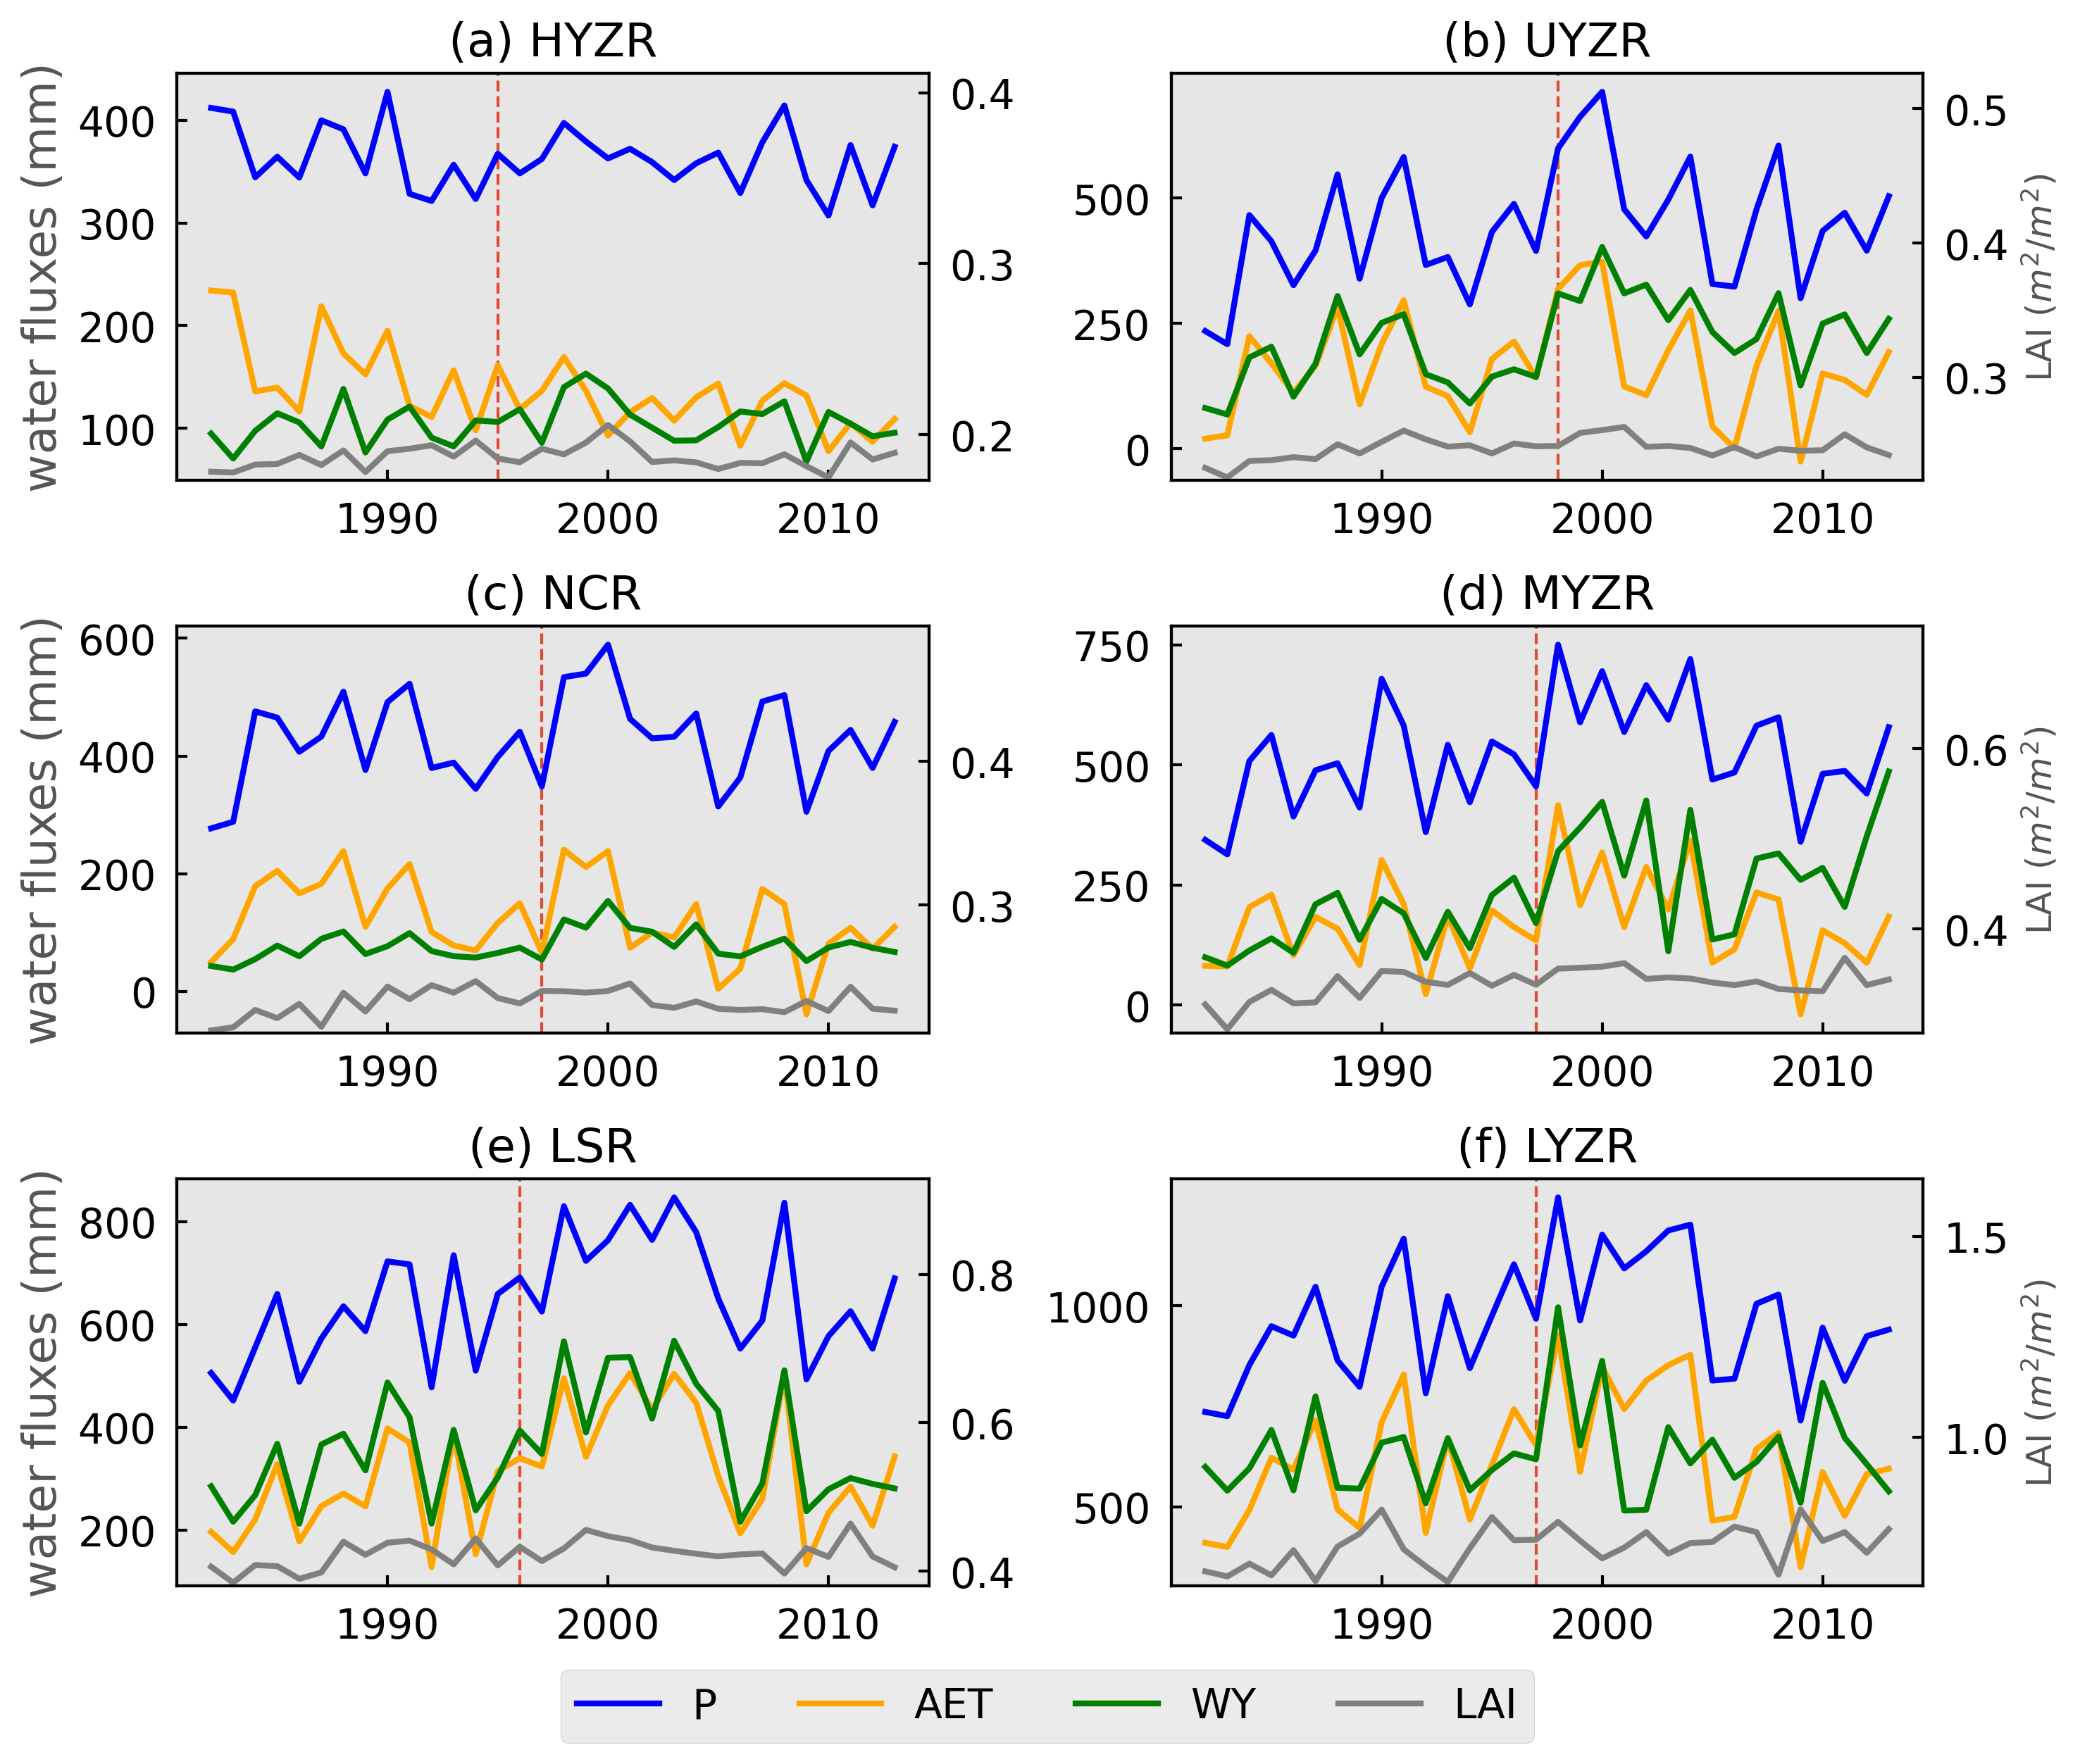
\includegraphics[width=12cm]{02-figures/time-series.png}
    \captionsetup{labelformat=empty}
    \caption{Figure \ref{figS:time series}. The temporal changes of precipitation (P, blue line), actual evaporation (AET, orange line), and water yield (WY, green line) and Leaf Area Index (LAI, grey line) during 1982--2013 in the entire UBR basin. The vertical line indicates the turning point in WY.}
\end{figure*}

\point{Figure S2 belongs in the paper in my opinion, as it seems like this is your main plot, which all following plots refer to.}
\reply{We thank the reviewer for this suggestion. In the revision, we place a schematic diagram (Figure \ref{fig:example_DMC}) in main text, which will explain how to conduct the DMC analysis more clearly.}

\point{Figure 1: Please change this 3D pie chart to bar char, as those are much easier to read.}
\reply{Thank you for pointing it out. We have placed Figure 1c into the supplementary (Figure \ref{figS:lucc}), and provided detailed information in Table \ref{tab: table 1} in the revised manuscript.}

\begin{figure*}[ht]
    \centering
    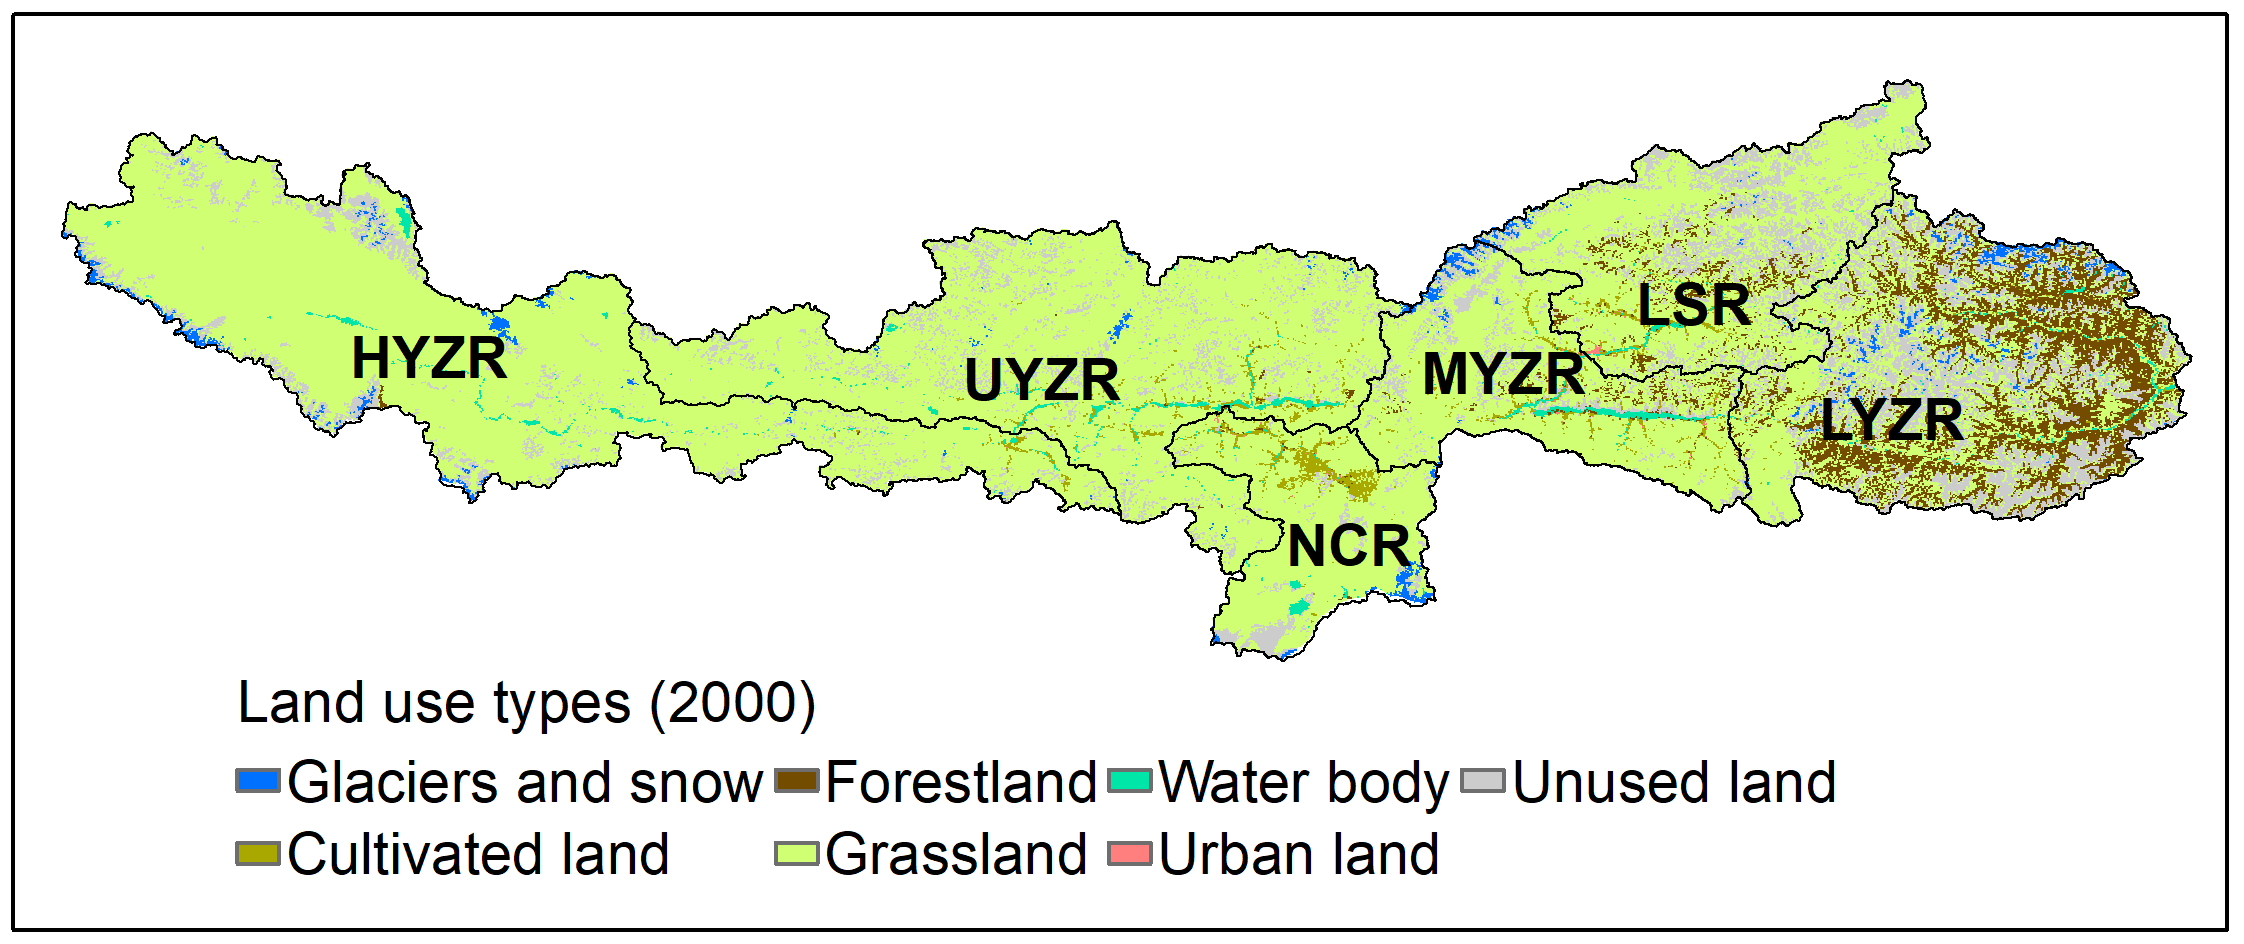
\includegraphics[width=8cm]{02-figures/lucc2000.png}
    \captionsetup{labelformat=empty}
    \caption{Figure \ref{figS:lucc}. The land use types in 2000 in the UBR basin.}
\end{figure*}

\point{Do the abbreviations that are used to label the subcatchments have any meaning?}
\reply{Yes. For example, "HYZR" means the headwater watershed in the Yarlung Zangbo River (YZR) basin, and "LSR" means Lasha River basin. We add detailed introduction for abbreviations in Table \ref{tab: table 1} in main text.}

\begin{table}[ht]
    \centering
    \caption{Information of six basins divided by the locations of hydrological stations.   
    The column "TP" indicates the turning point using the Pettitt method, in which a significant tuning point is labeled with *.
    Glaciers and snow area is acquired from the land use and cover in 2000 (see details in Dataset).}
    
    \begin{tabular}{ccccccc}
    \hline
    Abbrevation &
      Full names &
      Station &
      \begin{tabular}[c]{@{}c@{}}Total \\ area (km$^2$)\end{tabular} &
      \begin{tabular}[c]{@{}c@{}}Mean \\ elevation (m)\end{tabular} &
      \begin{tabular}[c]{@{}c@{}}Glaciers and snow \\ percentage (\%)\end{tabular} &
      \begin{tabular}[c]{@{}c@{}}TP\end{tabular} \\ \hline
    HYZR & Headstream    & Lhatse   & 49,739 & 5061 & 1.7  & 1995  \\
    UYZR & Upstream      & Nugesha  & 43,916 & 4985 & 0.39 & 1998* \\
    NCR  & Nianchu River & Shigatse & 14,359 & 4733 & 1.96 & 1997* \\
    MYZR & Midstream     & Yangcun  & 20,004 & 4681 & 1.81 & 1997* \\
    LSR  & Lhasa River   & Lhasa    & 25,601 & 4879 & 0.72 & 1996  \\
    LYZR & Downstream    & Nuxia    & 45,017 & 4586 & 2.51 & 1997  \\ \hline
    \end{tabular}
\end{table}

\point{Did you check if you evapotransporiration is roughly correct? You used evapotransporation data from a global model, which might have not been calibrated well to regions such extreme as yours.}
\reply{We thank the reviewer for pointing this out. As we do not have access to observed actual evaporation data in this region, we used AET from GLEAM, which has been extensively validated across varied vegetation types in China and has shown good performance with in situ observations \citep{yang2017multi}.}

\revised{83--85}{Regional actual evaporation (AET) with a 0.25$^{\circ}$ spatial resolution is acquired from Global Land Evaporation Amsterdam Model (GLEAM) \citep{martens2017gleam}. The evaporation product has been validated in different biome types in China and shown high correlations with in-situ eddy covariance AET \citep{yang2017multi}.}

\nextreply{Also, we discuss data uncertainties in the revised version.}

\revised{256--263}{Compared with precipitation, the estimation of evaporation may be much more challenging in high mountains. Although GLEAM actual evaporation shows the good agreement with in-situ eddy covariance records \citep{yang2017multi}, its model structure does not include wind speed and solar radiation, which may affect the estimation of sublimation, and thus total evaporation \citep{li2019evapotranspiration}. 
In addition, the coarse spatial resolution with a 0.25$^{\circ}$ spatial resolution in GLEAM may be insufficient to estimate regional evaporation in the UBR basin. 
However, with the help of the Second Tibetan Plateau Scientific Expedition and Research, the observation networks in meteorology, cryosphere and hydrology will be built, which is expected to benefit reliable precipitation and evaporation estimation, and make developing physically-based cryosphere-hydrological modeling possible \citep{wang2022observing}.}

\point{Why did you choose LAI as a proxy for vegetation and not some other measure?}
\reply{Thanks for your questions about the selections of vegetation indices. We give the reasons in the revised version.}

\revised{114--117}{LAI quantifies the amount of leaf area in an ecosystem and becomes an important variable reflecting vegetation structures and biophysical processes \citep{fang2019overview, forzieri2020increased}, and \citet{li2021vegetation} has used LAI to investigate vegetation effects on seasonal hydrology in the UBR basin.}

\point{Have you considered also checking for the runoff-ratio? This seems like a variable that should give you some additional information.}
\reply{We thank the reviewer for this suggestion. As effective precipitation is one of the main explanatory variable considered in this study, we decided to use just water yield, or runoff depth as the target variable. This allows us to robustly apply the statistical method (DMC) to quantify hydrological responses to climate warming.}

\point{Please change Fig. 3 and Fig 4. to boxplots or swarmplots (depending on your sample size you calculated your mean and standard deviation from). Having just a bar plot with a standard deviation does not really show how your underlying data looks like.}
\reply{We agree with the reviewer. We have changed the two figures to boxplots to support our analysis. Note the labelled numbers have been changed (Figure \ref{fig:magnitude-direction} and \ref{fig:attribution-magnitude}).}

\begin{figure*}[ht]
    \centering
    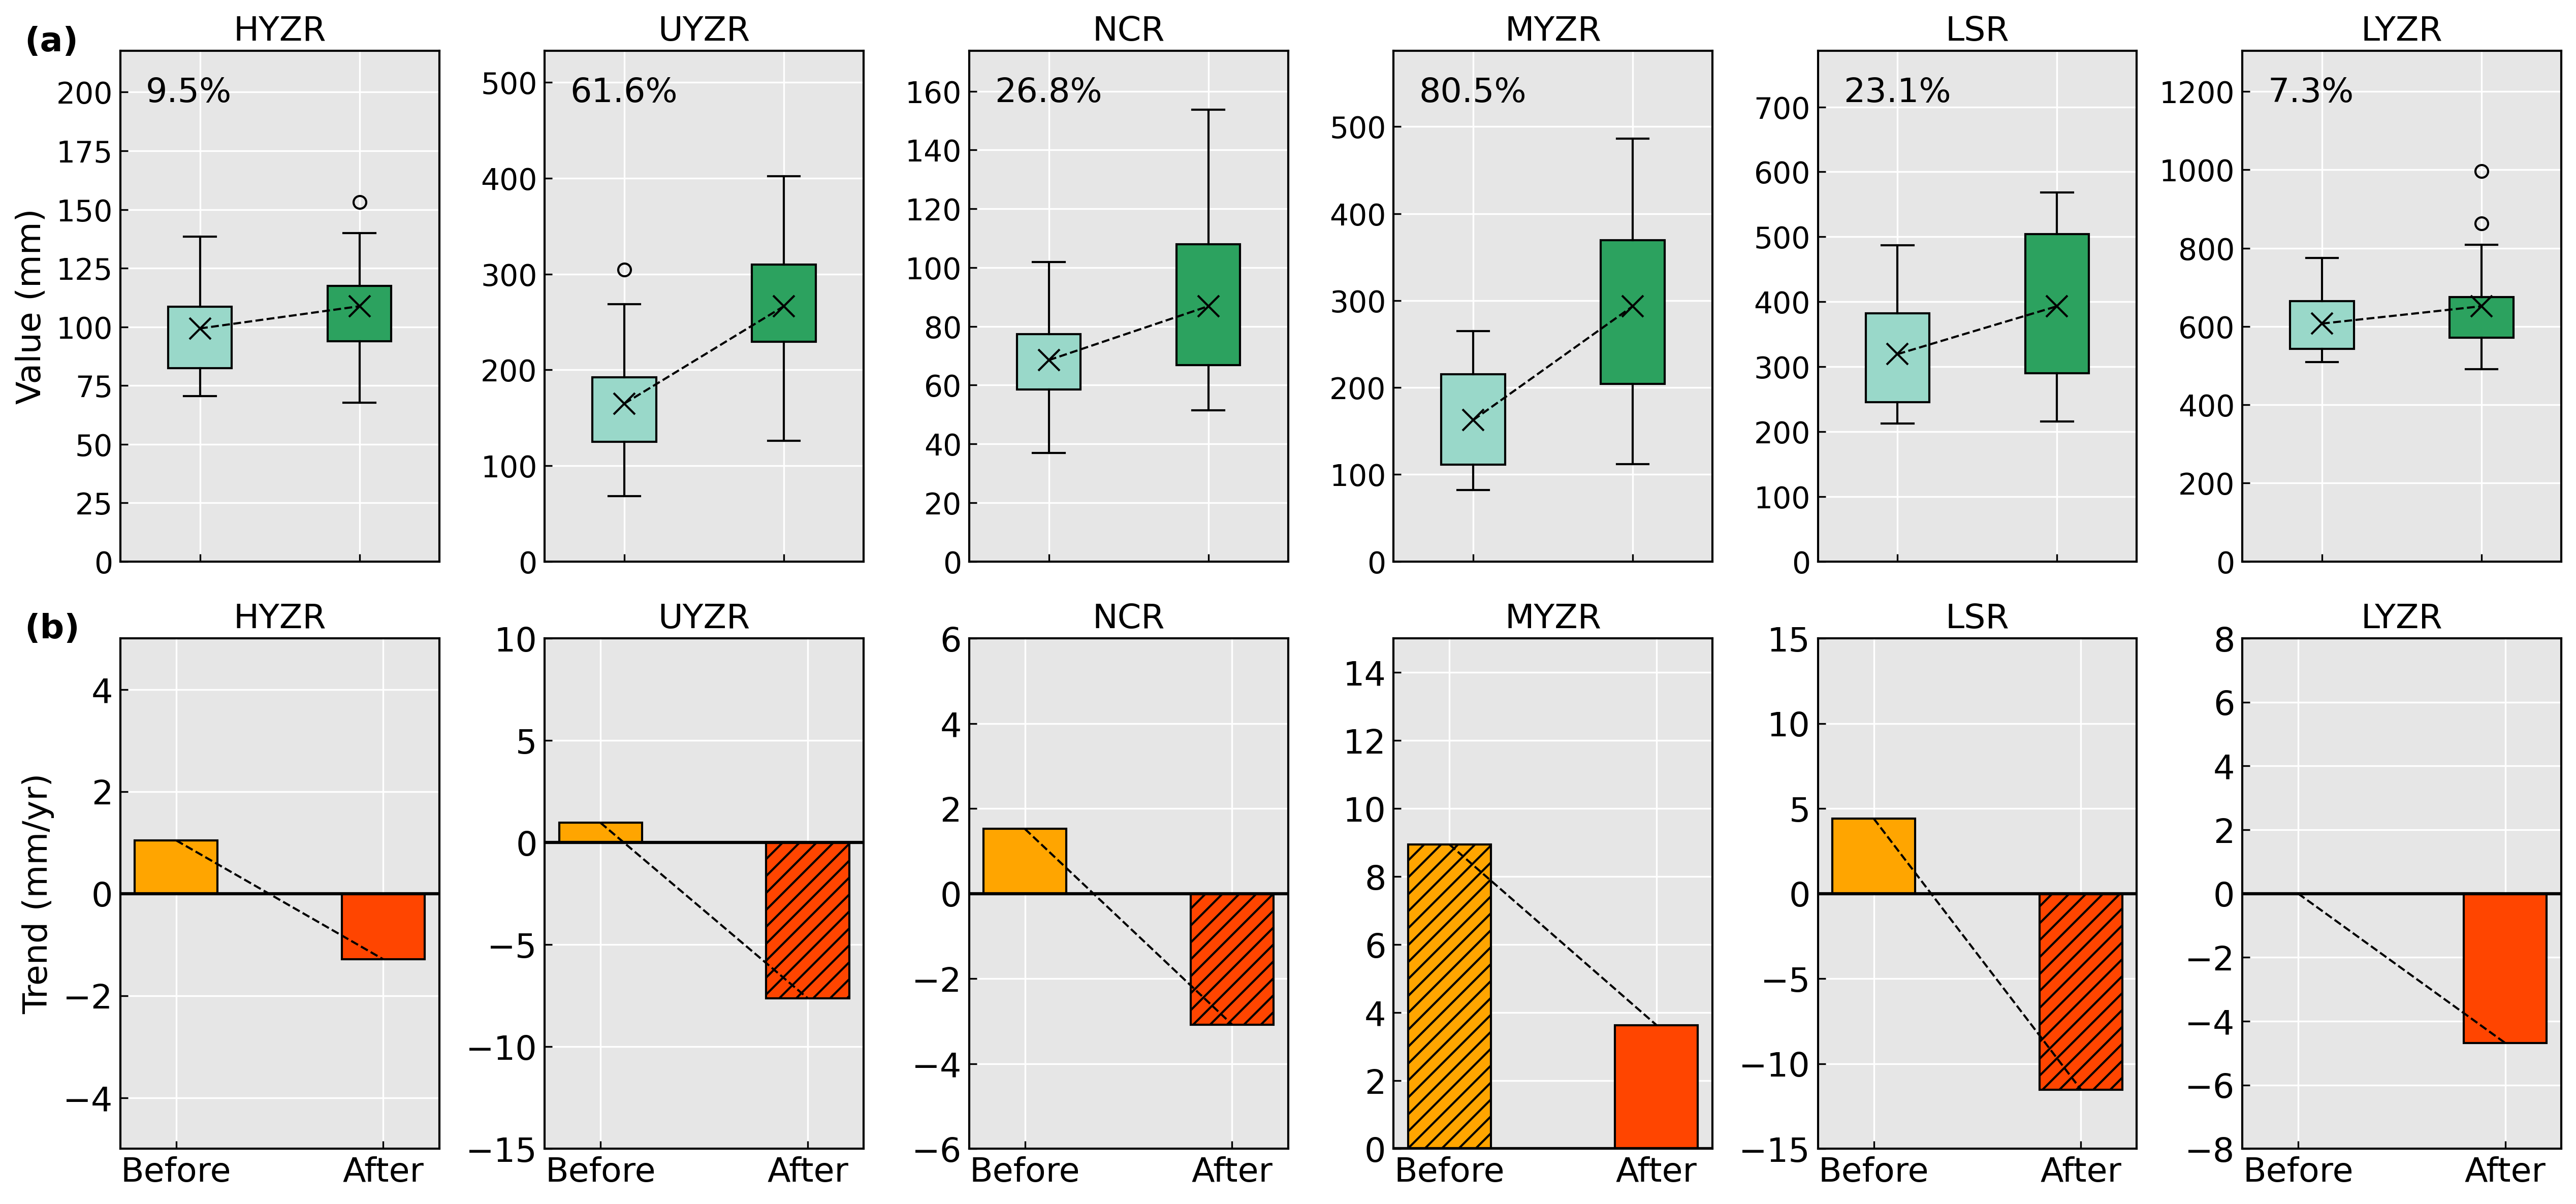
\includegraphics[width=8cm]{02-figures/magnitude_and_direction.png}
    \captionsetup{labelformat=empty}
    \caption
    {Figure \ref{fig:magnitude-direction}. Water yield regime shifts in the entire UBR basin. 
    (a) Magnitude of water yield changes. Black "x" signals show the mean of water yield in each boxplot.  
    (b) Direction of water yield changes. The black hatching represents the statistically significant trend (p $<$ 0.05).
    The color of boxes represents the period before (light color) and after (dark color) the turning point (TP).}
\end{figure*}

\begin{figure*}[ht]
    \centering
    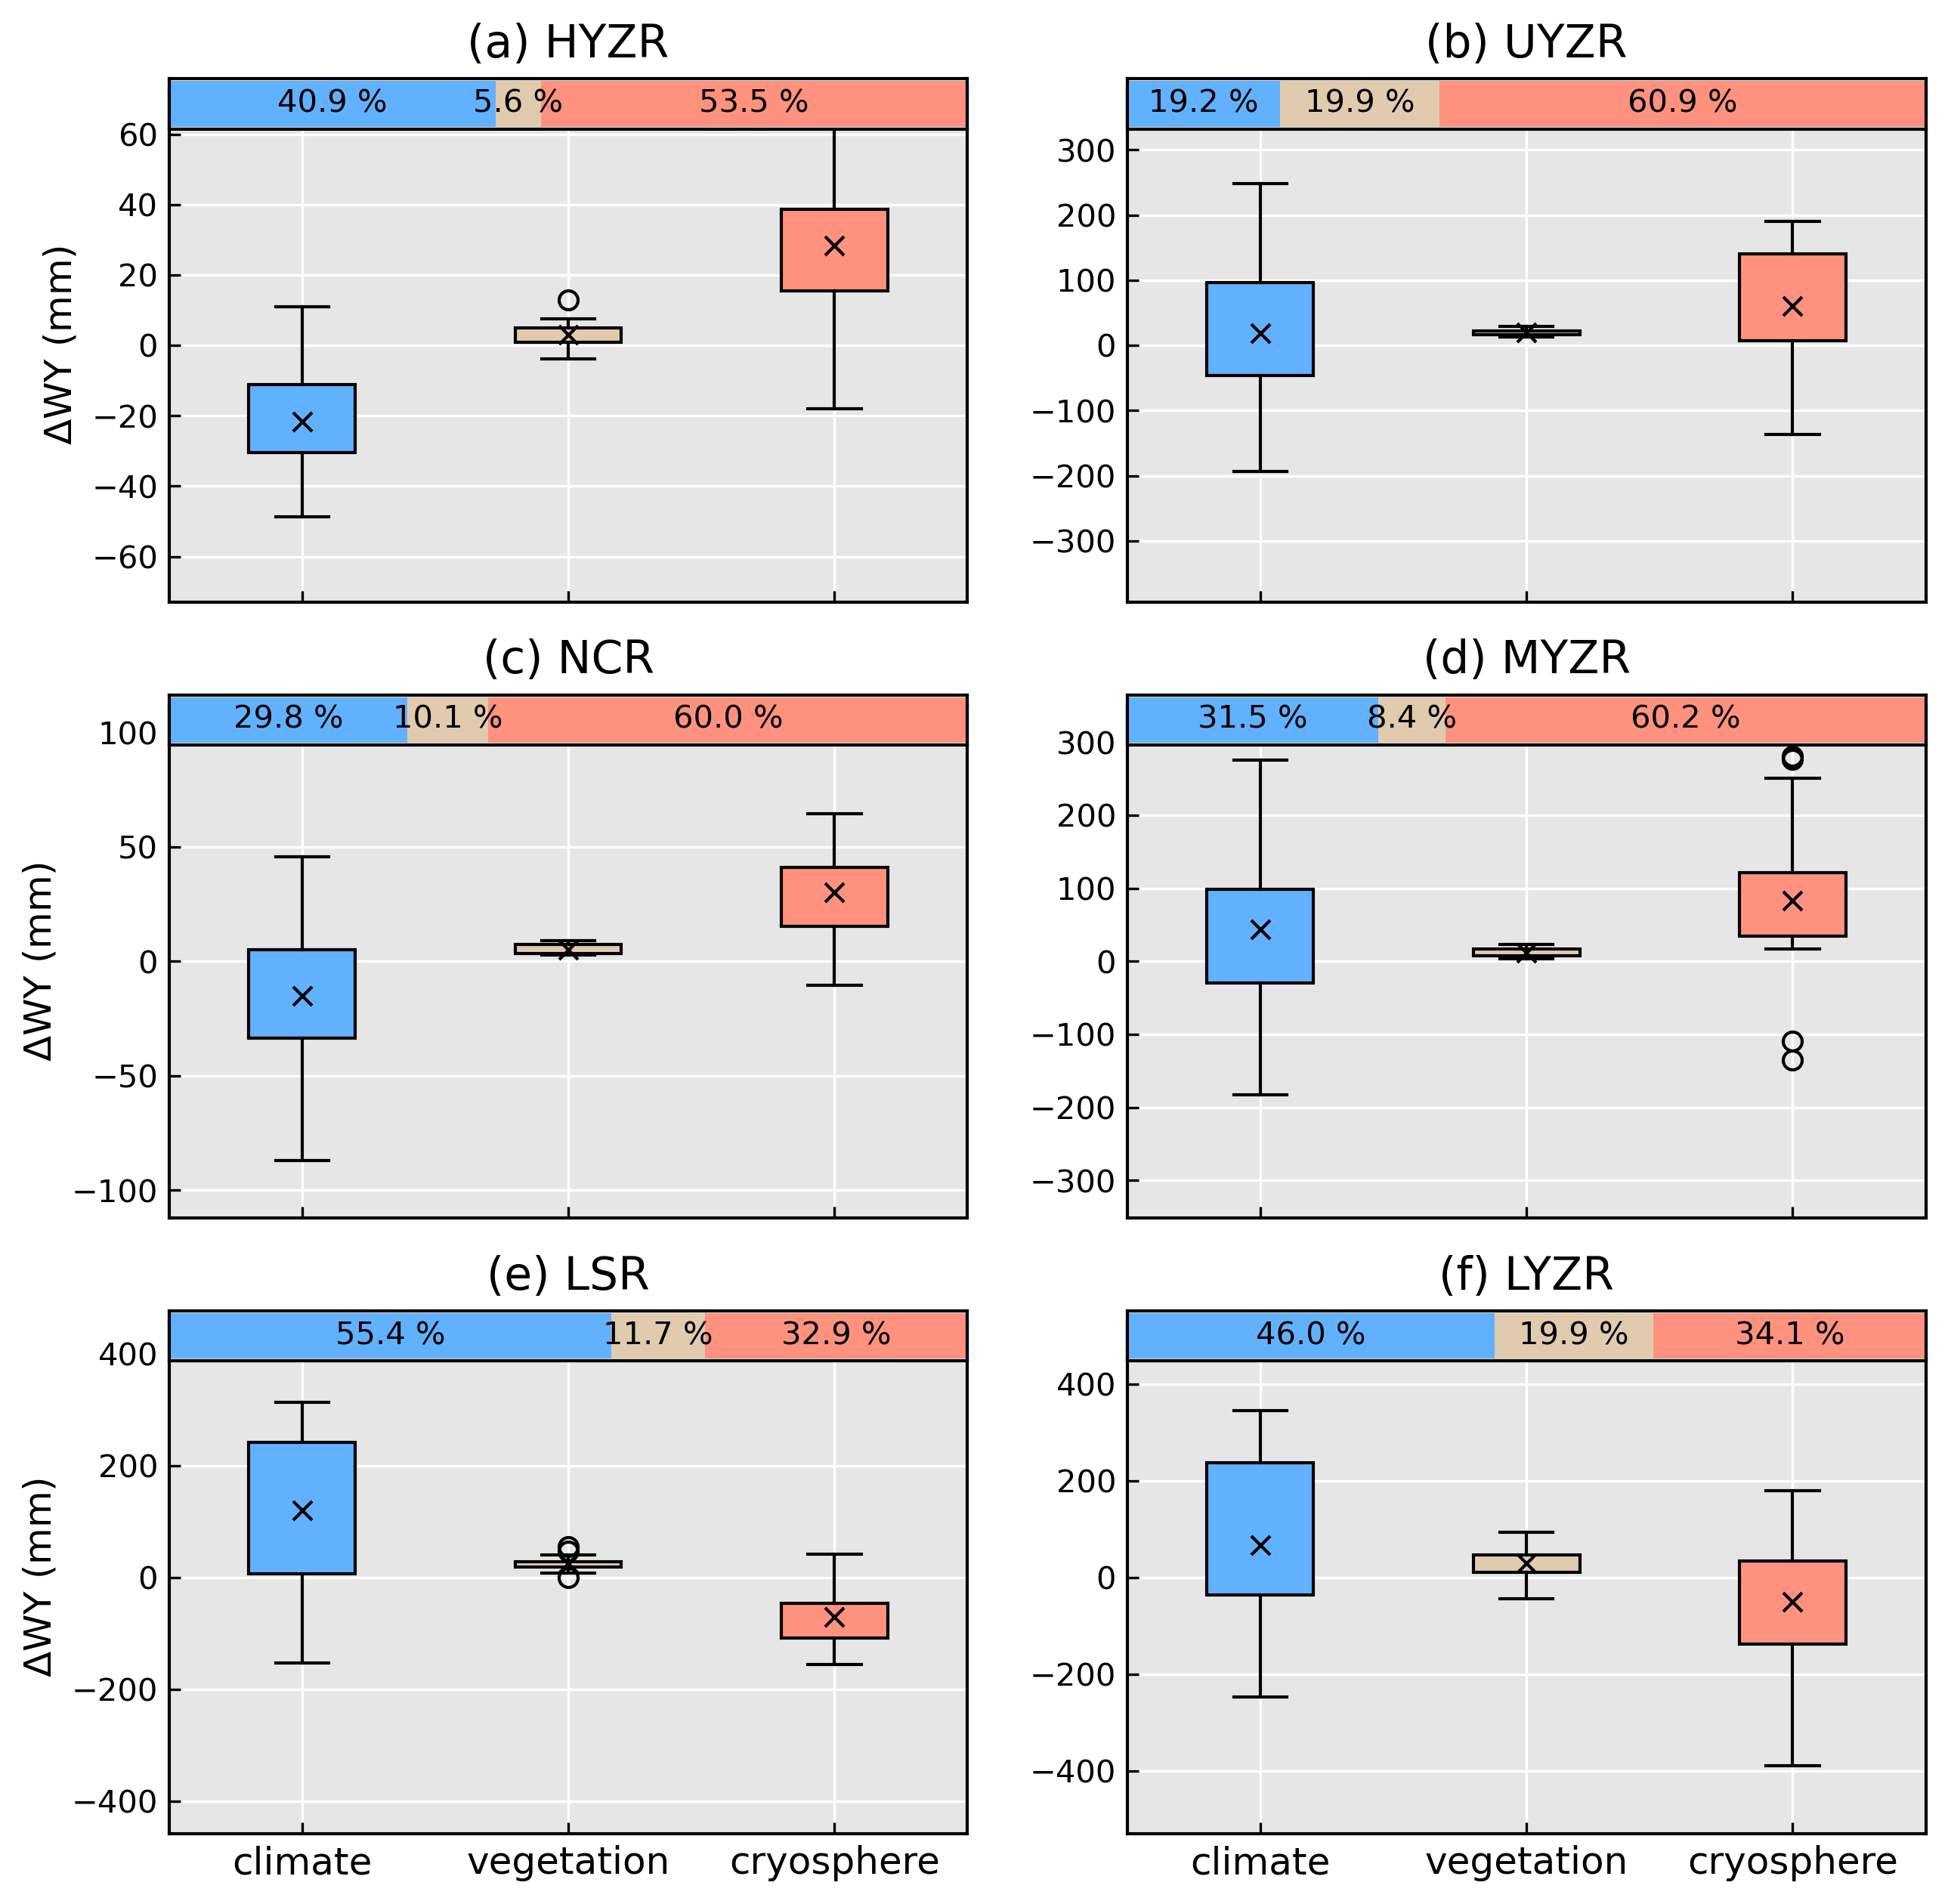
\includegraphics[width=8cm]{02-figures/attribution-in-magnitude.png}
    \captionsetup{labelformat=empty}
    \caption{Figure \ref{fig:attribution-magnitude}. Attribution analysis of magnitude increases in water yield due to climate ($\Delta WY_c$, blue box), vegetation ($\Delta WY_v$, tan box), and cryosphere ($\Delta WY_g$, red box), and their relative contributions (the bar with colors on the top) in each basin. Black "x" signals show the mean of water yield deviations (see Figure \ref{fig:attribution-results}) in each boxplot.}
\end{figure*}

\point{Are your p-values corrected? If not, this would mean that likely in Figure 5 there are way fewer significant trends.}
\reply{Thanks for your comments. The p value here is correct, but I am sorry that the labelled $n$ is wrong due to a minor programming error. In the revised version, we have corrected this error, and will only show the regression lines in Figure \ref{fig:attribution-direction} when p value is less than 0.05, and use "significant" or "significantly" in main text. For example:}

\begin{figure*}[ht]
    \centering
    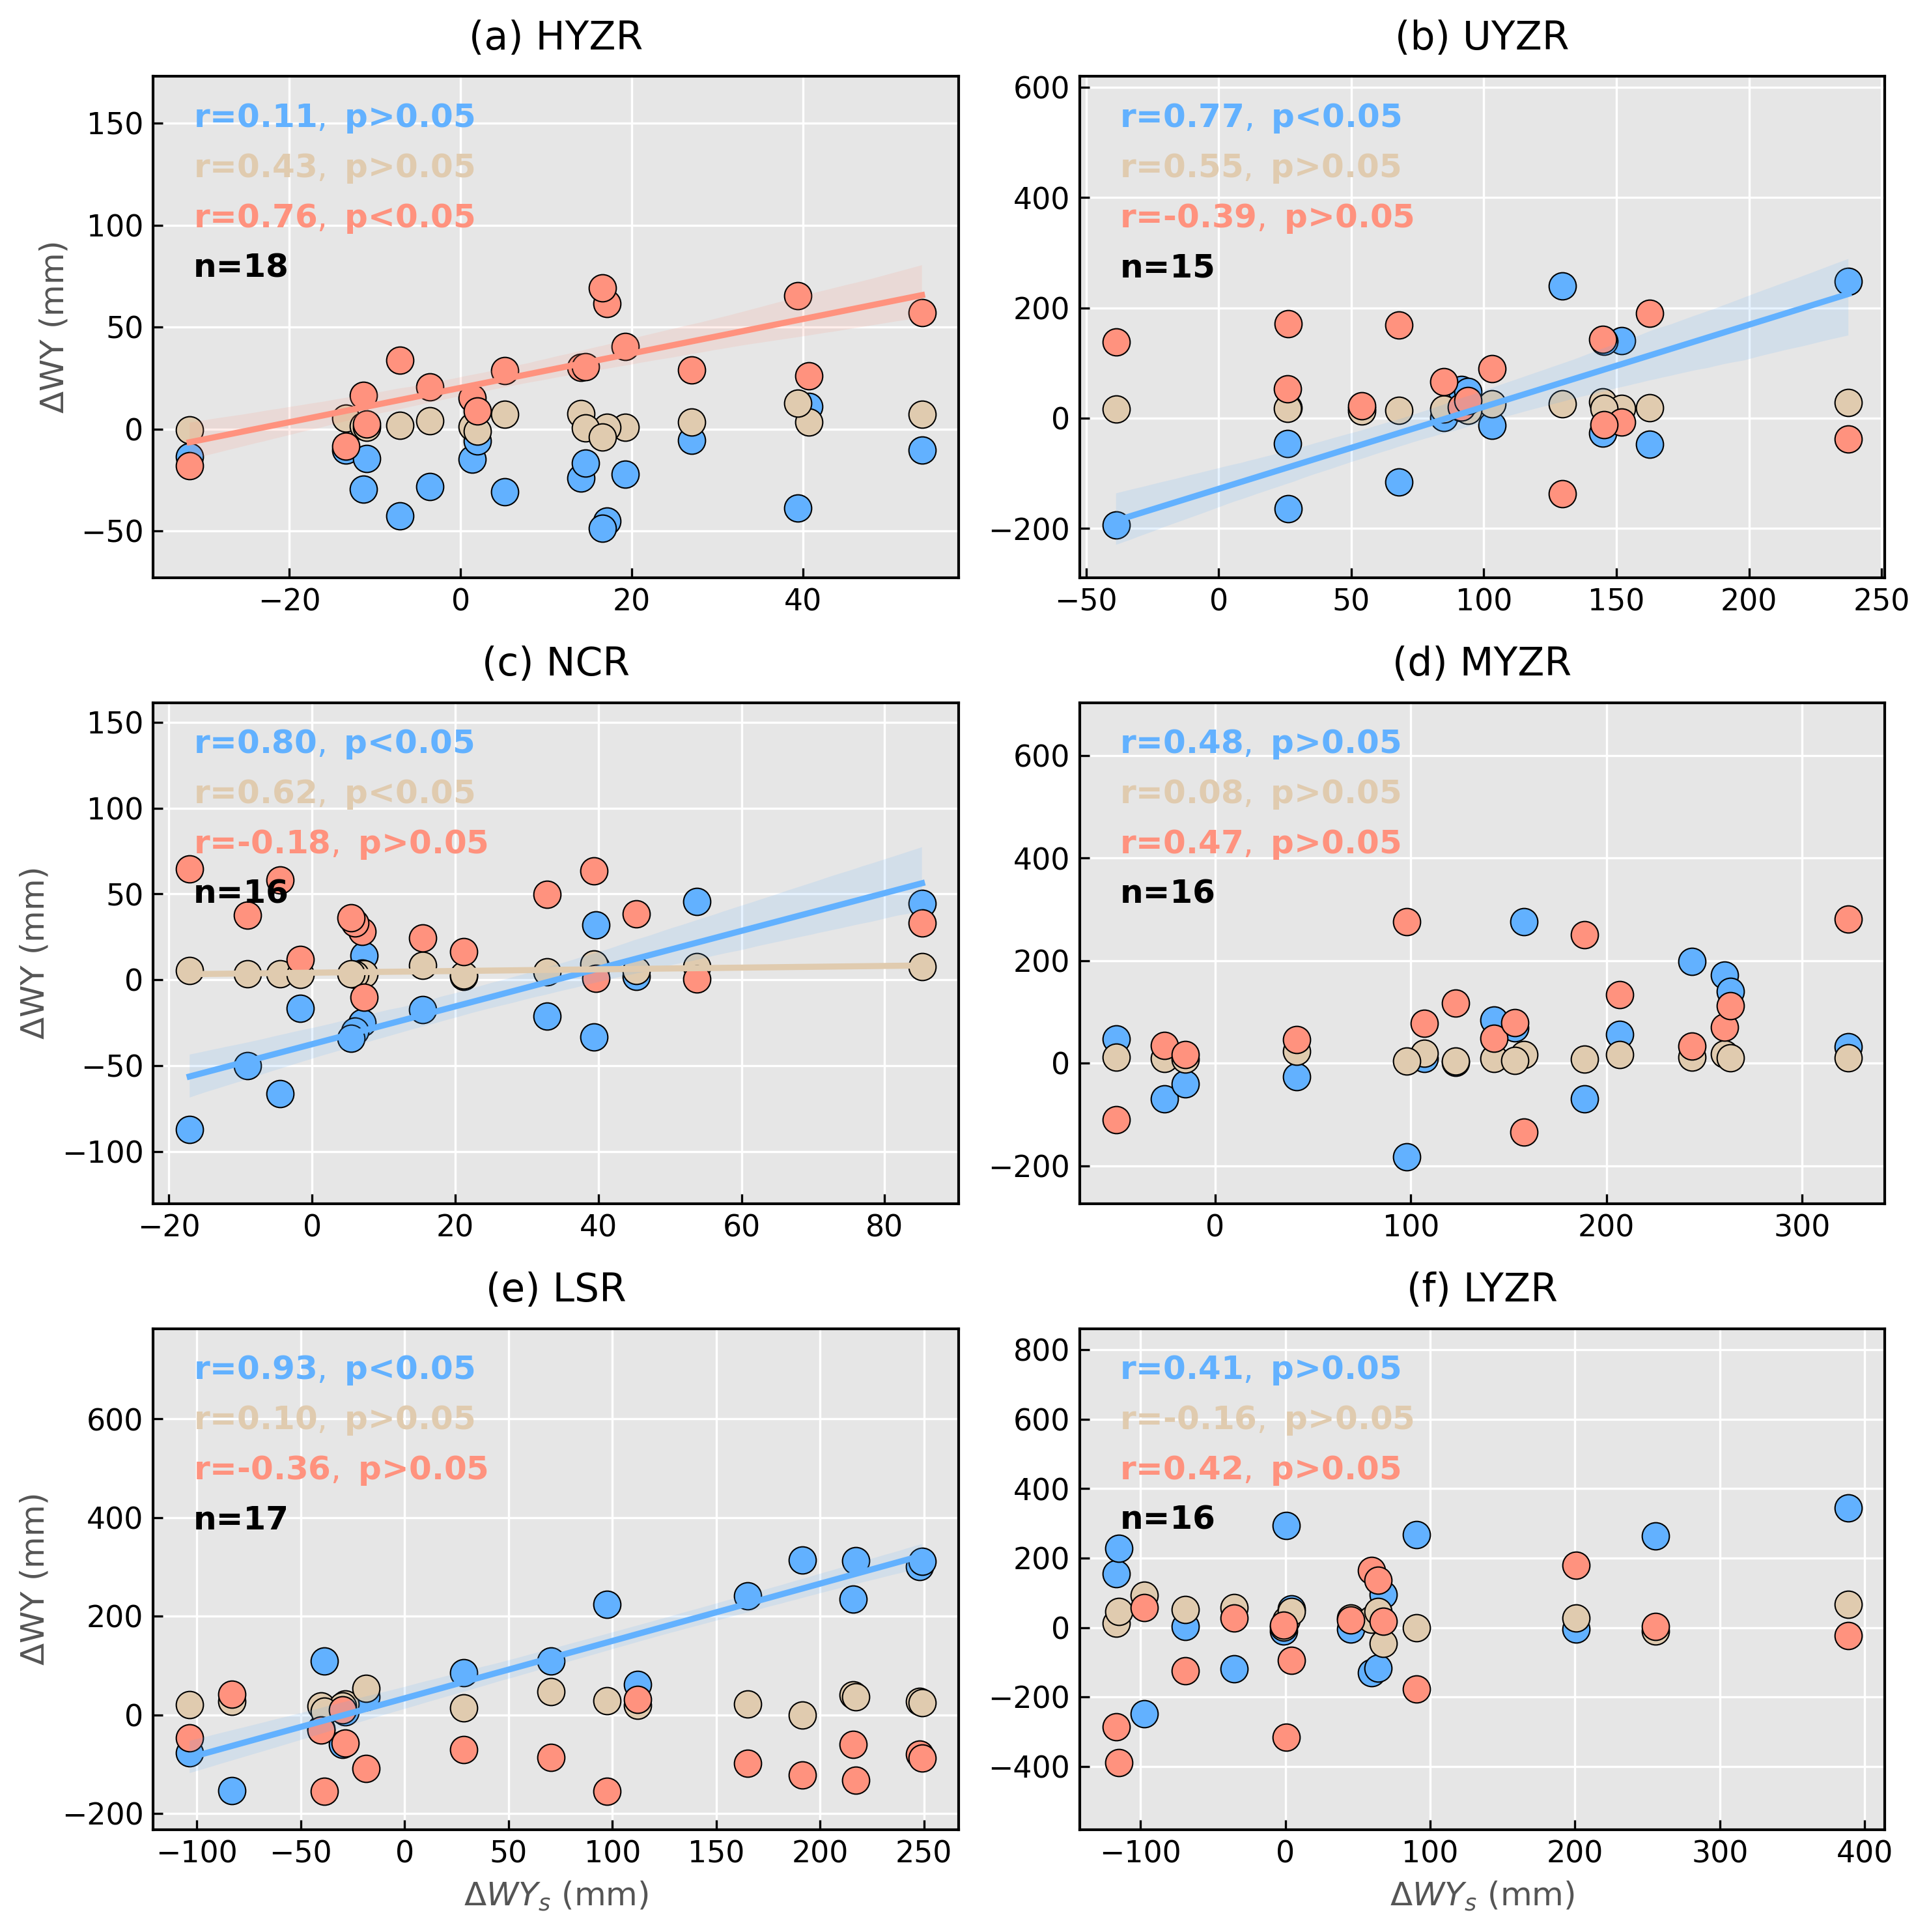
\includegraphics[width=12cm]{02-figures/contribution-relations.png}
    \captionsetup{labelformat=empty}
    \caption{Figure \ref{fig:attribution-direction}. The correlation between time series of total water yield deviation ($\Delta WY_s(t)$, x-axis) and its components (y-axis) caused by climate ($\Delta WY_c(t)$, blue point), vegetation ($\Delta WY_v(t)$, tan point), and cryosphere ($\Delta WY_g(t)$, red point), respectively.
    The fitting line and its 95\% confidence interval are shown only when p value $<$ 0.05. $n$ indicates the number of years after the TP, which is determined by the Pettitt method (See Table \ref{tab: table 1} and Figure \ref{fig:water-yield}c).}
\end{figure*}

\revised{191-192}{..., climate typically is \ul{positively associated} with total WY, in which the correlation is \ul{significant in half of basins} (p $<$ 0.05), ...}

\revised{198-199}{The  \ul{negative butweak relationship} indicates that melt waters from cryospheric loss may compensate for low flow, and even mitigate water shortage risks.}

\point{The text is quite heavy on abbreviations, which makes it harder to read. Please consider just writing the words out instead of abbreviating them.}
\reply{Thank you for the suggestions. We have deleted some abbreviations in main text, such as "Third Pole (TP)". And we also provide a table (see Table \ref{tab: table 1} in main text) to indicate some abbreviations clearly.}

\sect{Technical corrections}

\point{L19-21: I am not able to parse this sentence.}
\reply{We thank the reviewer for pointing this out. We have rewritten the abstract and convey the main information clearer to readers.}

\revised{1--12}{Although evidence of hydrological responses to climate is abundant, the reliable assessments of water yield (WY) over mountainous regions, such as the Upper Brahmaputra River (UBR) basin, remain unclear due to intensified cryospheric changes. 
Based on multi-station runoff observations, we examine long-term WY changes during 1982--2013 in the  UBR basin, and find there are in general hydrological regime shifts in the late 1990s; 
magnitude increases in WY range from $\sim$10\% to $\sim$80\%, while its directions reverse from upward to downward after the late 1990s.
Then, the double mass curve (DMC) technique is used to assess the effects of climate, vegetation, and cryosphere on WY changes. 
Results show that climate and cryosphere together contribute to over 80\% of magnitude increases of WY in the entire UBR basin, in which the role of vegetation is nearly negligible.
The combined effects, however, are either offsetting or additive, leading to slight or substantial magnitude increases, respectively. 
Climate change, particularly precipitation decrease leads to the downward WY trend in recent years,
while melt waters under global warming may alleviate the water shortage in some basins. 
Therefore, the combined effects of climate and cryosphere on WY should be considered in future water resources management over mountainous basins, particularly involving co-benefits between upstream and downstream regions.}

\point{L45: would delete this mention of “Third Pole” as this exact phrasing has already been used in the paragraph above it.}
\reply{Thanks for your comment. We have deleted it.}

\bibliographystyle{copernicus}
\bibliography{reference.bib}

%%%%%%%%%%%%%%%%%%%%%%%%%%%%%%%%%%%%%%%%%%%%%%
%%%%%%%%%%%%%%%%%%%%%%%%%%%%%%%%%%%%%%%%%%%%%%
%%%%%%%%%%%%%%%%%%%%%%%%%%%%%%%%%%%%%%%%%%%%%%
\reviewersection

\point{The manuscript from Li et al. offers an analysis of the different drivers of hydrological regime shifts in the upper Brahmaputra, highlighting changing climate and glacier loss as major determinants. While the work is generally well written and shaped, there are some issues/suggestions to be considered before publication:}
\reply{We thank the reviewer for their constructive comments and specifically for the suggestions on using the idea of "peak water" as a conceptual framework for understanding cryospheric contributions to river flow. \textbf{We will clarify some definitions, and give related evidence with "peak water" in Results and Discussion.}.}

\sect{General Comments}

\point{A conceptual framework would greatly help you to shape the storyline. Actually, there are several studies showing regime shifts associated with glacier loss (see Huss \& Hoch, 2018; concept of “peak water”). I think that your work provides further evidence in that direction, showing the magnitude of hydrological glacier influence over spatial gradients, and offering an important analysis of the turning points in regime shifts.}
\reply{We thank the reviewer for suggestions. We have now framed our analysis and discussion within the conceptual framework of "peak water" as you suggested. For example,}

\revised{197--209}{In contrast to positive contributions of climate, we find that WY caused by cryosphere exhibits a negative association with reduced total WY deviations in recent years in the UYZR (r = -0.39, p $>$ 0.05) and LSR (r = -0.36, p $>$ 0.05) basins. 
\ul{The negative but weak relationship indicates that melt waters from cryospheric loss may compensate for low flow, and even mitigate water shortage risks.}
Also, the compensating effect from cryosphere is much stronger in the MYZR (r = 0.47, p $>$ 0.05), and together with climate contributions, contributes to the increasing WY trend (Figure \ref{fig:magnitude-direction}).
Different from other regions, however, the HYZR basin shows a significantly positive relationship between cryospheric contributions and total WY deviations (r = 0.76, p $<$ 0.05), indicating that cryosphere instead of climate leads to the downward trend in headwaters.
This signifies that in this region, \ul{cryospheric contributions have already passed a maximum supplying to river flow, due to decreased glaciers and snow under continuous warming.}
The is further verified by the relationship of cryospheric contributions to total WY ($RC_g$) with temperature (Figure \ref{figS:warming-and-cryosphere}). 
\ul{In the HYZR basin, WY resulting from the cryosphere continues to increase with temperature until a maximum is reached, beyond which cryospheric contribution to total WY begins to decrease.}
In addition, the compensating effect of melt waters can be seen clearly in the UYZR, MYZR and LSR basins, i.e., WY caused by cryospheric loss keeps a positive relationship with the increase of temperature, further supporting the higher correlation in these basins (Figure \ref{fig:attribution-direction}).}

\revised{227--233}{Cryospheric contribution is also important for water yield regime shifts -- \ul{melt waters from glaciers and snow melting can alleviate water resources shortages, mainly caused by decreased precipitation in recent years} (Figure \ref{fig:attribution-direction}+\ref{figS:climate-directions}). This finding is also supported by observed glacier runoff data \citep{yao2010glacial} and several modeling studies \citep{lutz2014consistent, Zhang2020VariationOM, wang2021tp}. 
However, after glacier runoff reaches a maximum, defined as "peak water" \citep{gleick2010peak}, \ul{cryospheric mass loss cannot sustain the rising melt waters with atmospheric warming} (e.g. the HYZR basin in Figure \ref{figS:warming-and-cryosphere}), which is in agreement with \citet{huss2018global}.}

\begin{figure*}[ht]
    \centering
    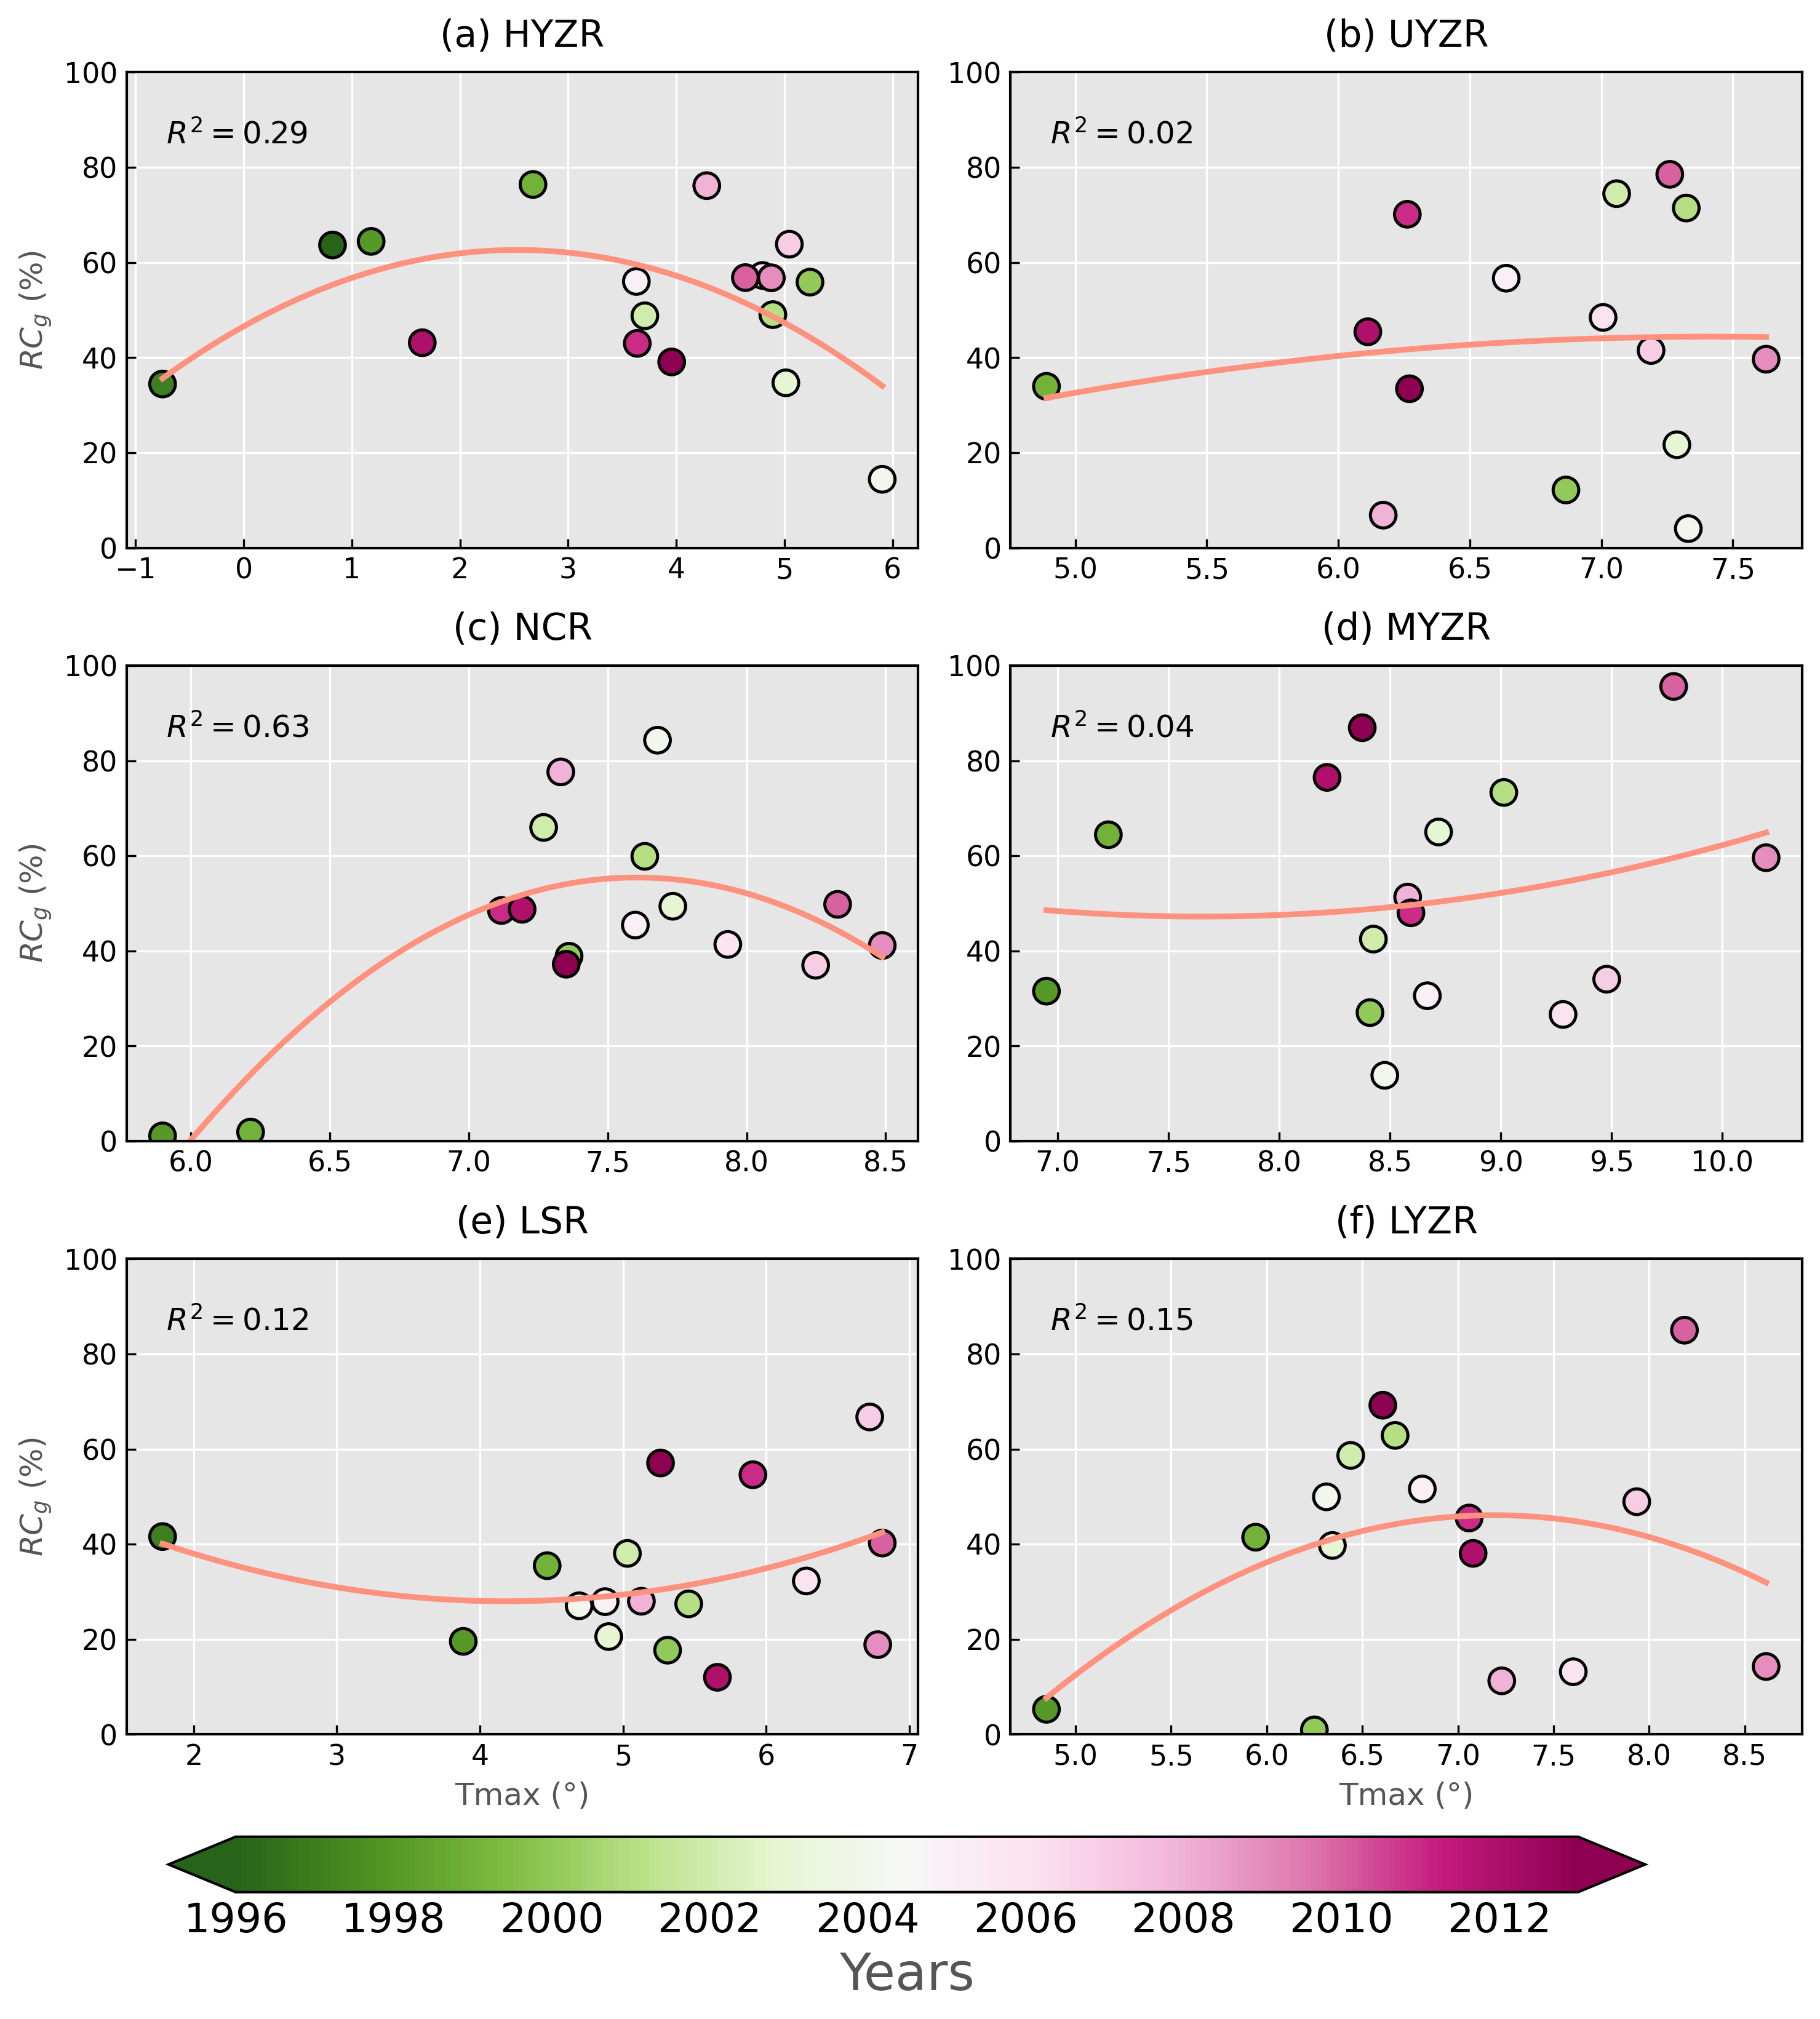
\includegraphics[width=8cm]{02-figures/peak-water-analysis.png}
    \captionsetup{labelformat=empty}
    \caption{Figure \ref{figS:warming-and-cryosphere}. The relationship between cryospheric contributions to water yield deviations ($RC_g(t)$, see Methods in main text) and annual mean 2m maximum air temperature ($T_{max}$) using the polynomial fitting. 
    The colorbar indicates the years after a TP in individual basins. 
    R square here used to evaluate the fitting goodness is labelled in each panel.}
\end{figure*}

\point{I found the discussion a little bit lacking. As glaciers ad the climate are the major hydrological drivers, what will it happen when glaciers disappear and the climate has shifted? Also, you should stress that the “climate shifts” are changes in precipitation patterns in your work.}
\reply{We thank the reviewer for pointing this out. We have added the detailed analysis and discussions within the framework of "peak water".}

\revised{201--207}{Different from other regions, however, the HYZR basin shows a significantly positive relationship between cryospheric contributions and total WY deviations (r = 0.76, p $<$ 0.05), indicating that cryosphere instead of climate leads to the downward trend in headwaters.
This signifies that in this region, \ul{cryospheric contributions have already passed a maximum supplying to river flow, due to decreased glaciers and snow under continuous warming.} 
The is further verified by the relationship of cryospheric contributions to total WY ($RC_g$) with temperature (Figure \ref{figS:warming-and-cryosphere}). 
\ul{In the HYZR basin, WY resulting from the cryosphere continues to increase with temperature until a maximum is reached, beyond which cryospheric contribution to total WY begins to decrease.}}

\revised{227--233}{Cryospheric contribution is also important for water yield regime shifts -- \ul{melt waters from glaciers and snow melting can alleviate water resources shortages, mainly caused by decreased precipitation in recent years} (Figure \ref{fig:attribution-direction}+\ref{figS:climate-directions}). This finding is also supported by observed glacier runoff data \citep{yao2010glacial} and several modeling studies \citep{lutz2014consistent, Zhang2020VariationOM, wang2021tp}. 
However, after glacier runoff reaches a maximum, defined as "peak water" \citep{gleick2010peak}, \ul{cryospheric mass loss cannot sustain the rising melt waters with atmospheric warming} (e.g. the HYZR basin in Figure \ref{figS:warming-and-cryosphere}), which is in agreement with \citet{huss2018global}.}

\nextreply{In the revised manuscript, we also stress the importance of precipitation on water yield.}

\revised{225--227}{\ul{Climate, especially precipitation, still control the declining WY trend after the TP in most regions} (Figure \ref{fig:attribution-direction} and \ref{figS:climate-directions}), may become an important factor in occurrence of turning points (Figure \ref{fig:water-yield}c+d).
\ul{This suggests the importance of precipitation and its projections on future hydrological process in mountainous watersheds} \citep{lutz2014consistent}.}

\begin{figure*}[ht]
    \centering
    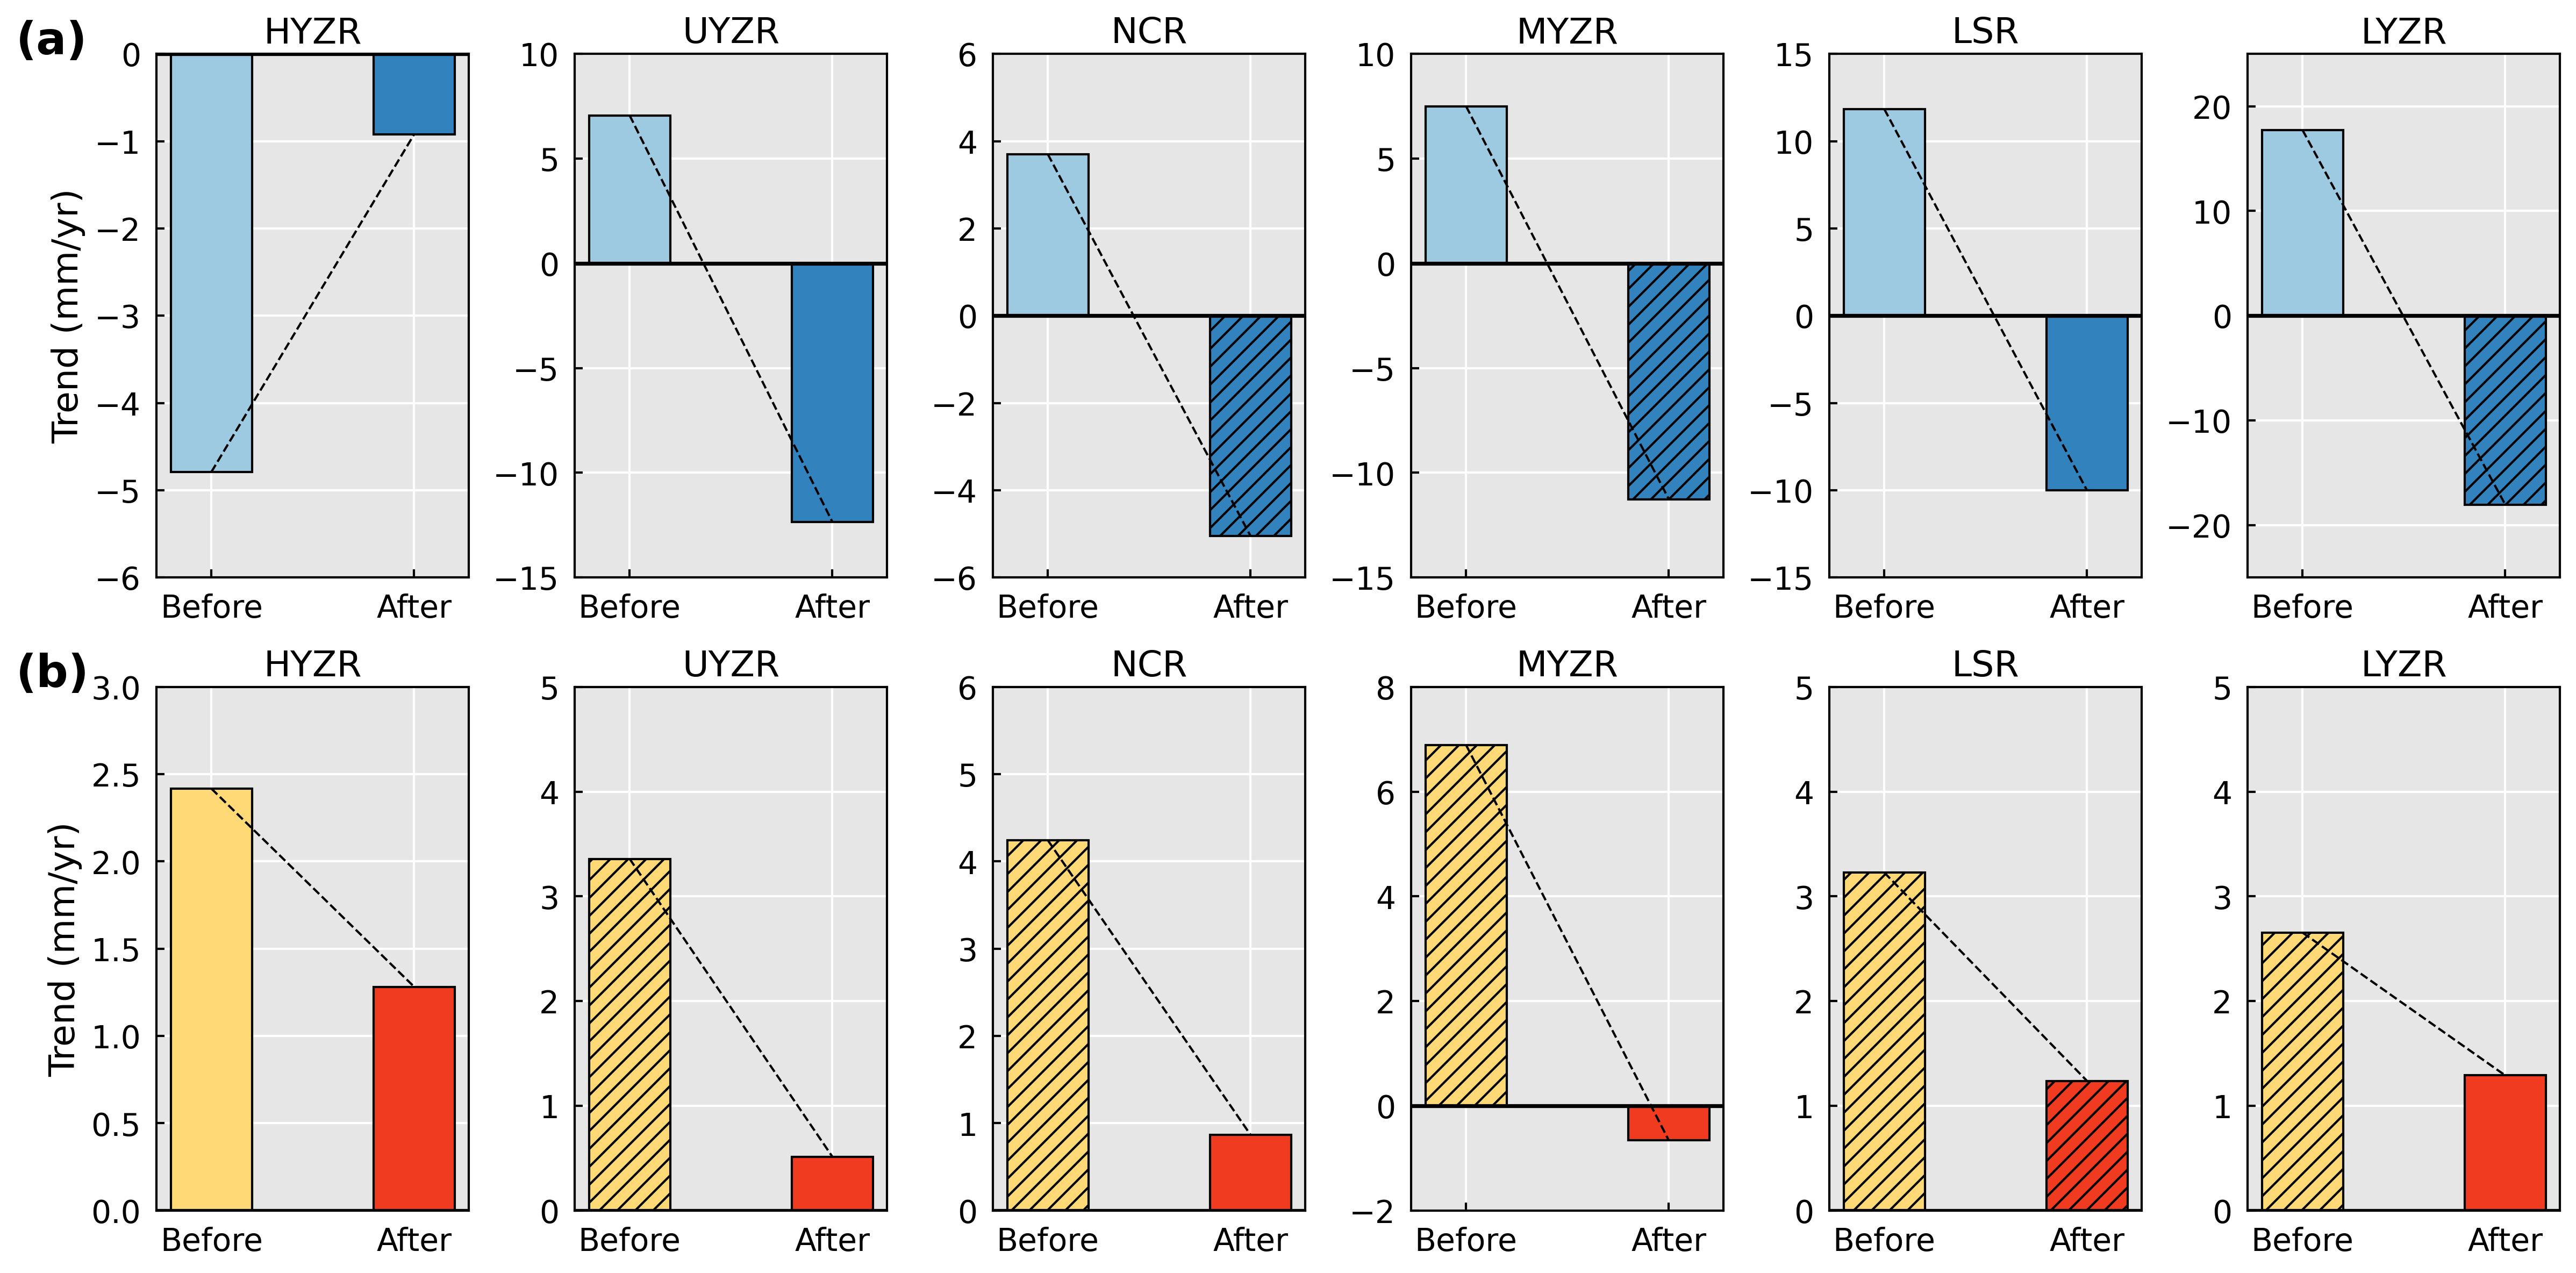
\includegraphics[width=8cm]{02-figures/P_AET_diections.png}
    \captionsetup{labelformat=empty}
    \caption{Figure \ref{figS:climate-directions}. Direction of precipitation (a) and actual evaporation (b) changes. 
    The black hatching represents the statistically significant trend (p $<$ 0.05).
    The color of boxes represents the period before
    (light color) and after (dark color) the turning point (TP).}
\end{figure*}

\point{Why did you choose this particular type of analysis to estimate drivers of regime changes? This is not sufficiently explained in the text}
\reply{Thank you for your suggestions. We have supplemented reasons and an example (Figure \ref{fig:example_DMC}) for the use of DMC method in the Introduction and Methodology sections.}

\revised{46--50}{Lastly, the present inadequate understanding of hydrological responses to complex interactions among climate, vegetation, and cryosphere \ul{limits the application of hydrological models in these mountainous watersheds} \citeprev{pellicciotti2012challenges}. 
While, long-term observed runoff records and recent high-resolution precipitation datasets \ul{give a pathway for using statistical methods} to estimate runoff responses to warming in the UBR basin. }

\begin{figure*}[ht]
    \centering
    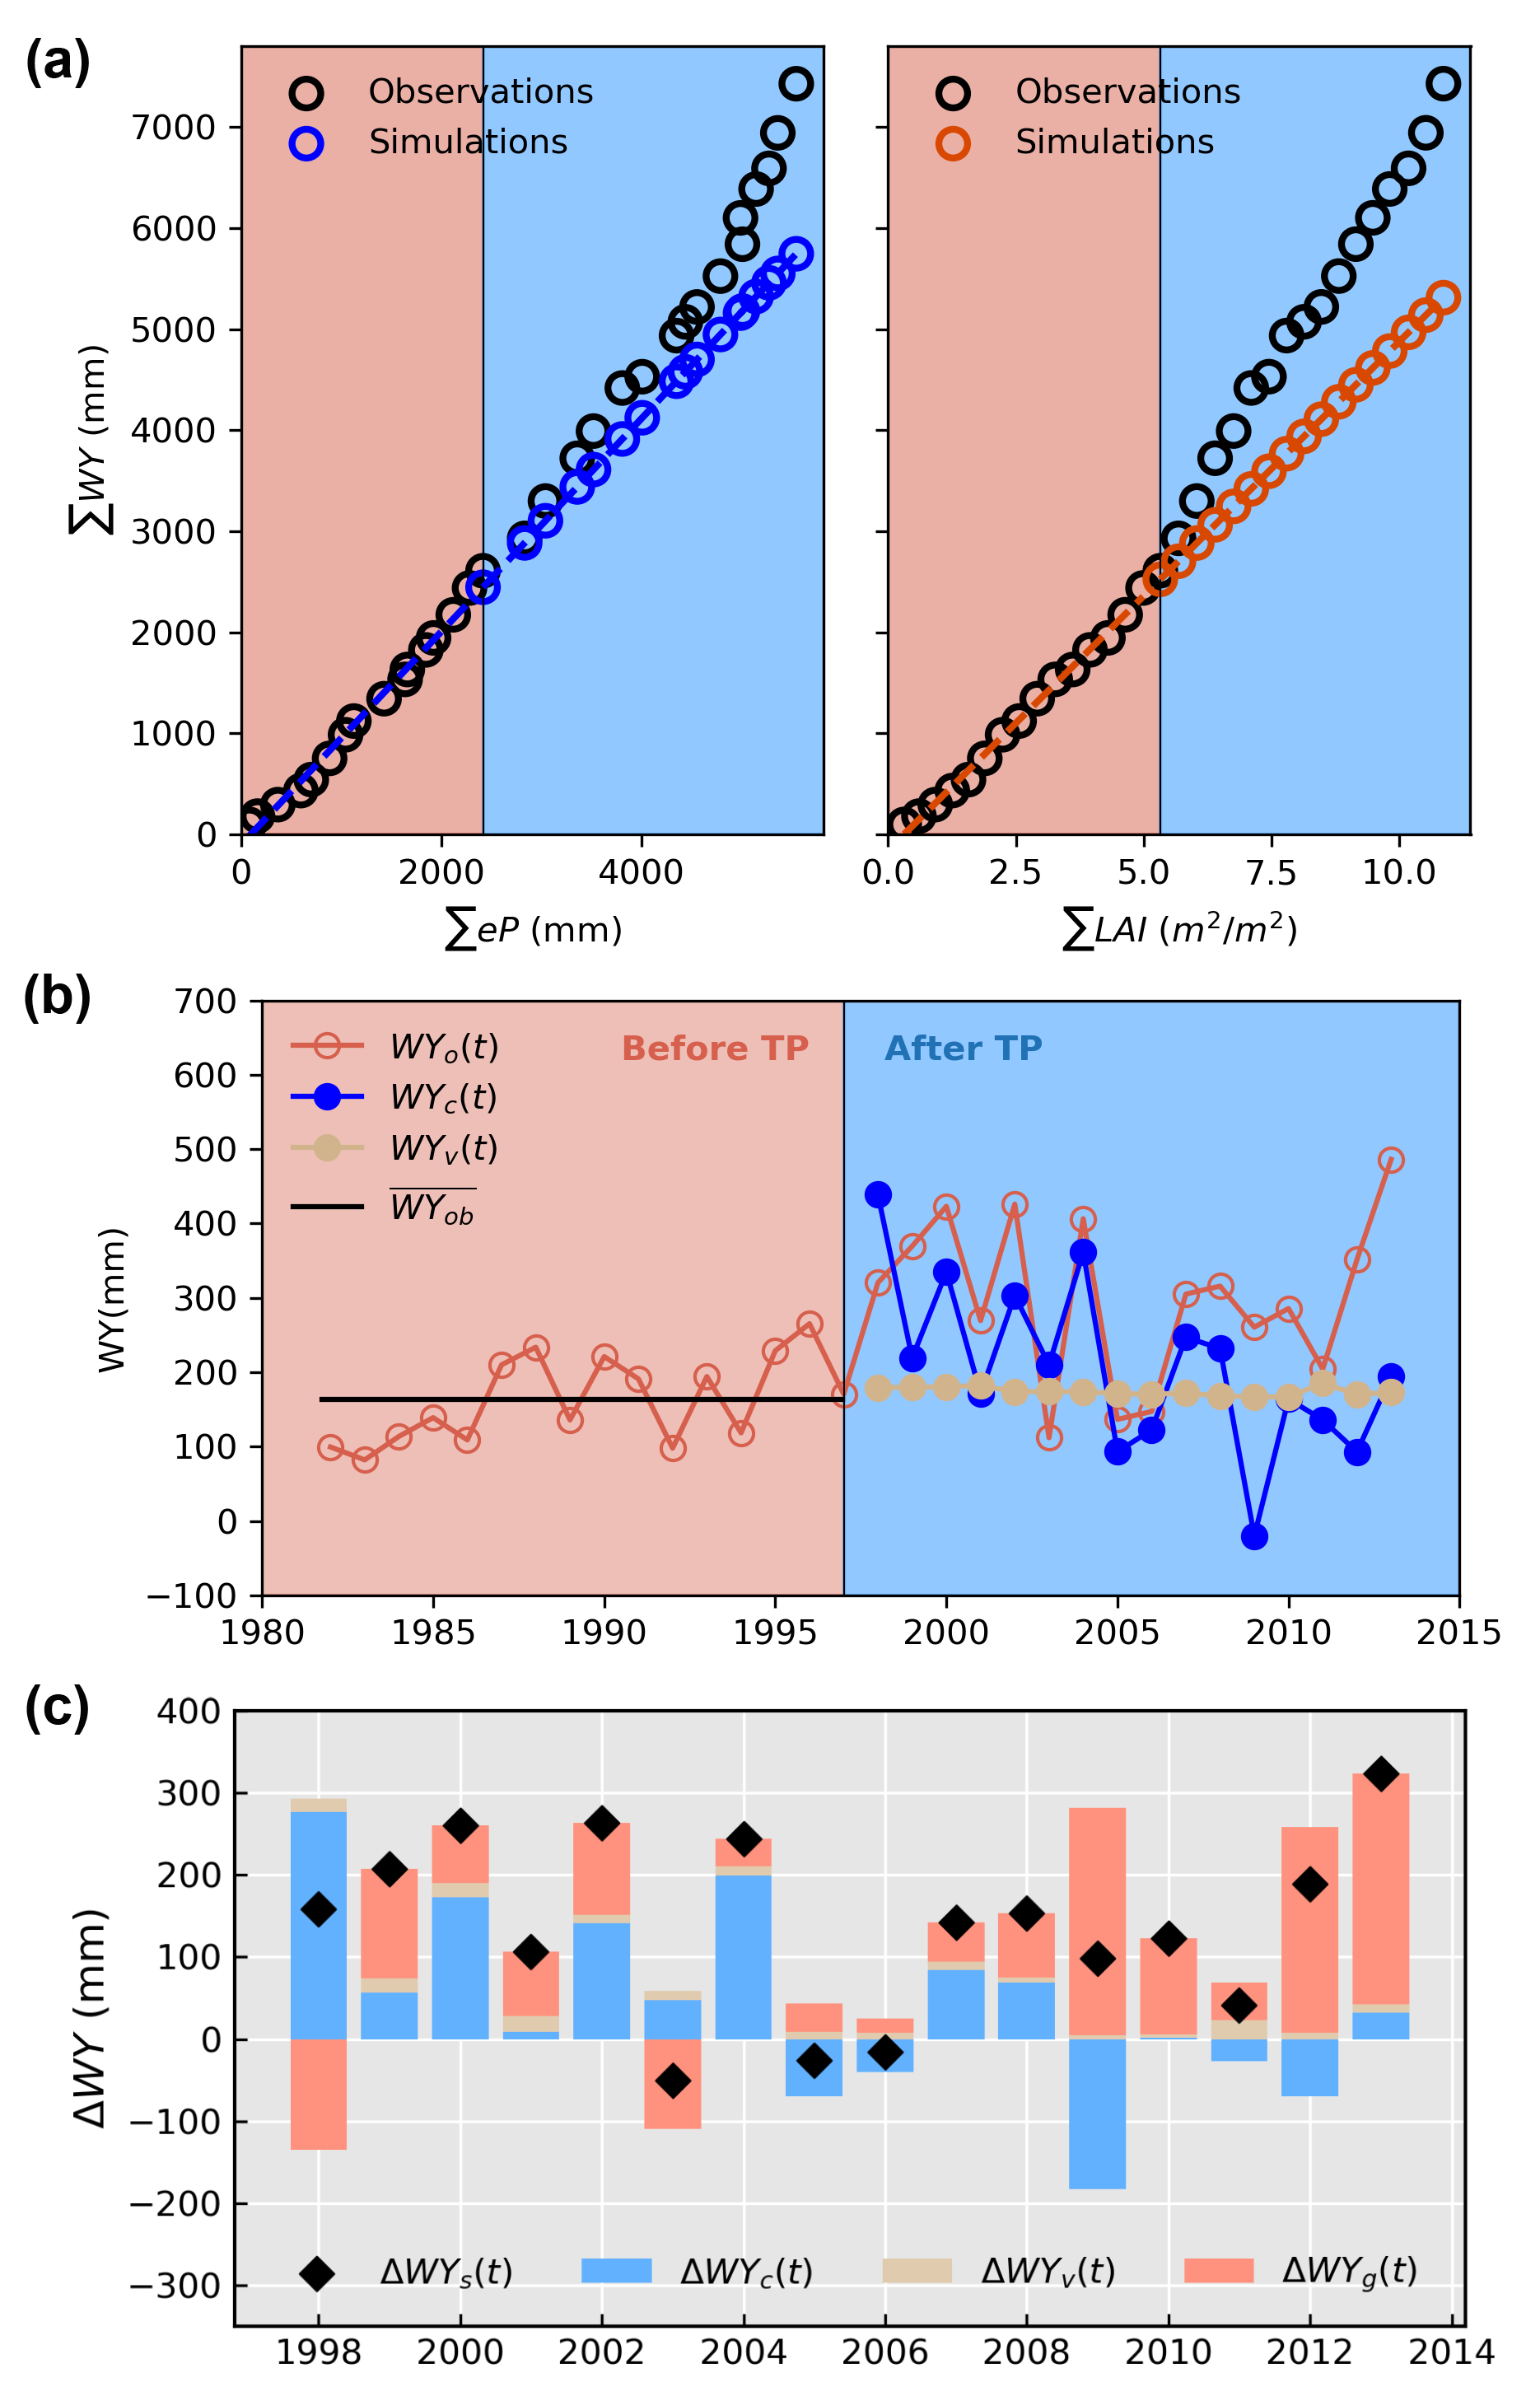
\includegraphics[width=8cm]{02-figures/example_DMC.png}
    \captionsetup{labelformat=empty}
    \caption
    {Figure \ref{fig:example_DMC}. The schematic diagram showing how to estimate the effects of climate, vegetation, and cryosphere on water yield in the MYZR basin (Details in Methodology).}
\end{figure*}

\revised{103--111}{The DMC used here is a plot of the cumulative data of one variable versus the cumulative data of another related variable in a concurrent period.
It has previously been used to assess the individual effect of climate \citeprev{gao2011changes}, forest disturbance \citeprev{wei2010quantifying}, wildfire \citep{hallema2018burned}, and cryosphere \citeprev{brahney2017determining} on water resources.
For the large and pristine UBR and other mountainous basins, climate, vegetation, and cryosphere (melt waters from glaciers and snow under warming, see \citealtrev{biemans2019importance,huss2018global}) play important roles in hydrology, and these three parts must be together considered to accurately estimate hydrological responses to warming. 
It is \ul{considerably hard to directly calculate the supply of melt waters to WY due to the lack of long-term glacier monitoring}, while runoff observations and high-resolution climate and vegetation data make it possible to use the DMC technique, \ul{a data-driven statistical method}, to estimate cryospheric contributions to WY.  }

\revised{112--118}{\ul{The selection of climate and vegetation} indices used in the DMC technique is an important issue.
Previous studies have shown that effective precipitation (eP, P-AET) can reflect more information of climate on WY compared with individual P or AET, and be regarded as a reliable proxy to climate \citeprev{wei2010quantifying,zhang2019separating}. 
LAI quantifies the amount of leaf area in an ecosystem and becomes an important variable reflecting vegetation structures and biophysical processes \citeprev{fang2019overview, forzieri2020increased}, and \citetrev{li2021vegetation} has used LAI to investigate vegetation effects on seasonal hydrology in the UBR basin. 
Hence, we consider eP and LAI as the indices of climate and vegetation respectively, and use their time series as the inputs in the DMC model.}

\revised{119--122}{\ul{To obtain cryospheric contributions to WY}, we firstly build two types of DMC plots (see Figure \ref{figS:DMC}) to assess the contributions of climate (eP) and vegetation (LAI), and then subtract the sum of estimated contributions from total WY deviations as cryospheric effects (results are shown in Figure \ref{fig:attribution-results}). The schematic diagram \ref{fig:example_DMC} and associated mathematical formulas are shown as follows:}

\point{It seems that the drivers of regime shifts depend on the considered part of the catchment. In general, the influence from glaciers is higher in the upper part and that from precipitation is higher at downstream locations. 
I think that translating this information into “spatial gradients/turning points” would greatly improve the quality of your work. 
Is there any relationship between the glacier cover in the catchment and the role of glaciers in driving the magnitude and direction of regime shifts associated with glacier loss or precipitation changes?}
\reply{The turning point is both controlled by climate and cryospheric loss, and thus it may be not possible to directly build relationships between turning points and cryospheric contributions. In addition, the limited data (we only access snow and glacier area in 2000) may hinder the analysis between glacier areas and cryospheric contributions from the DMC method.}

\begin{figure*}[ht]
    \centering
    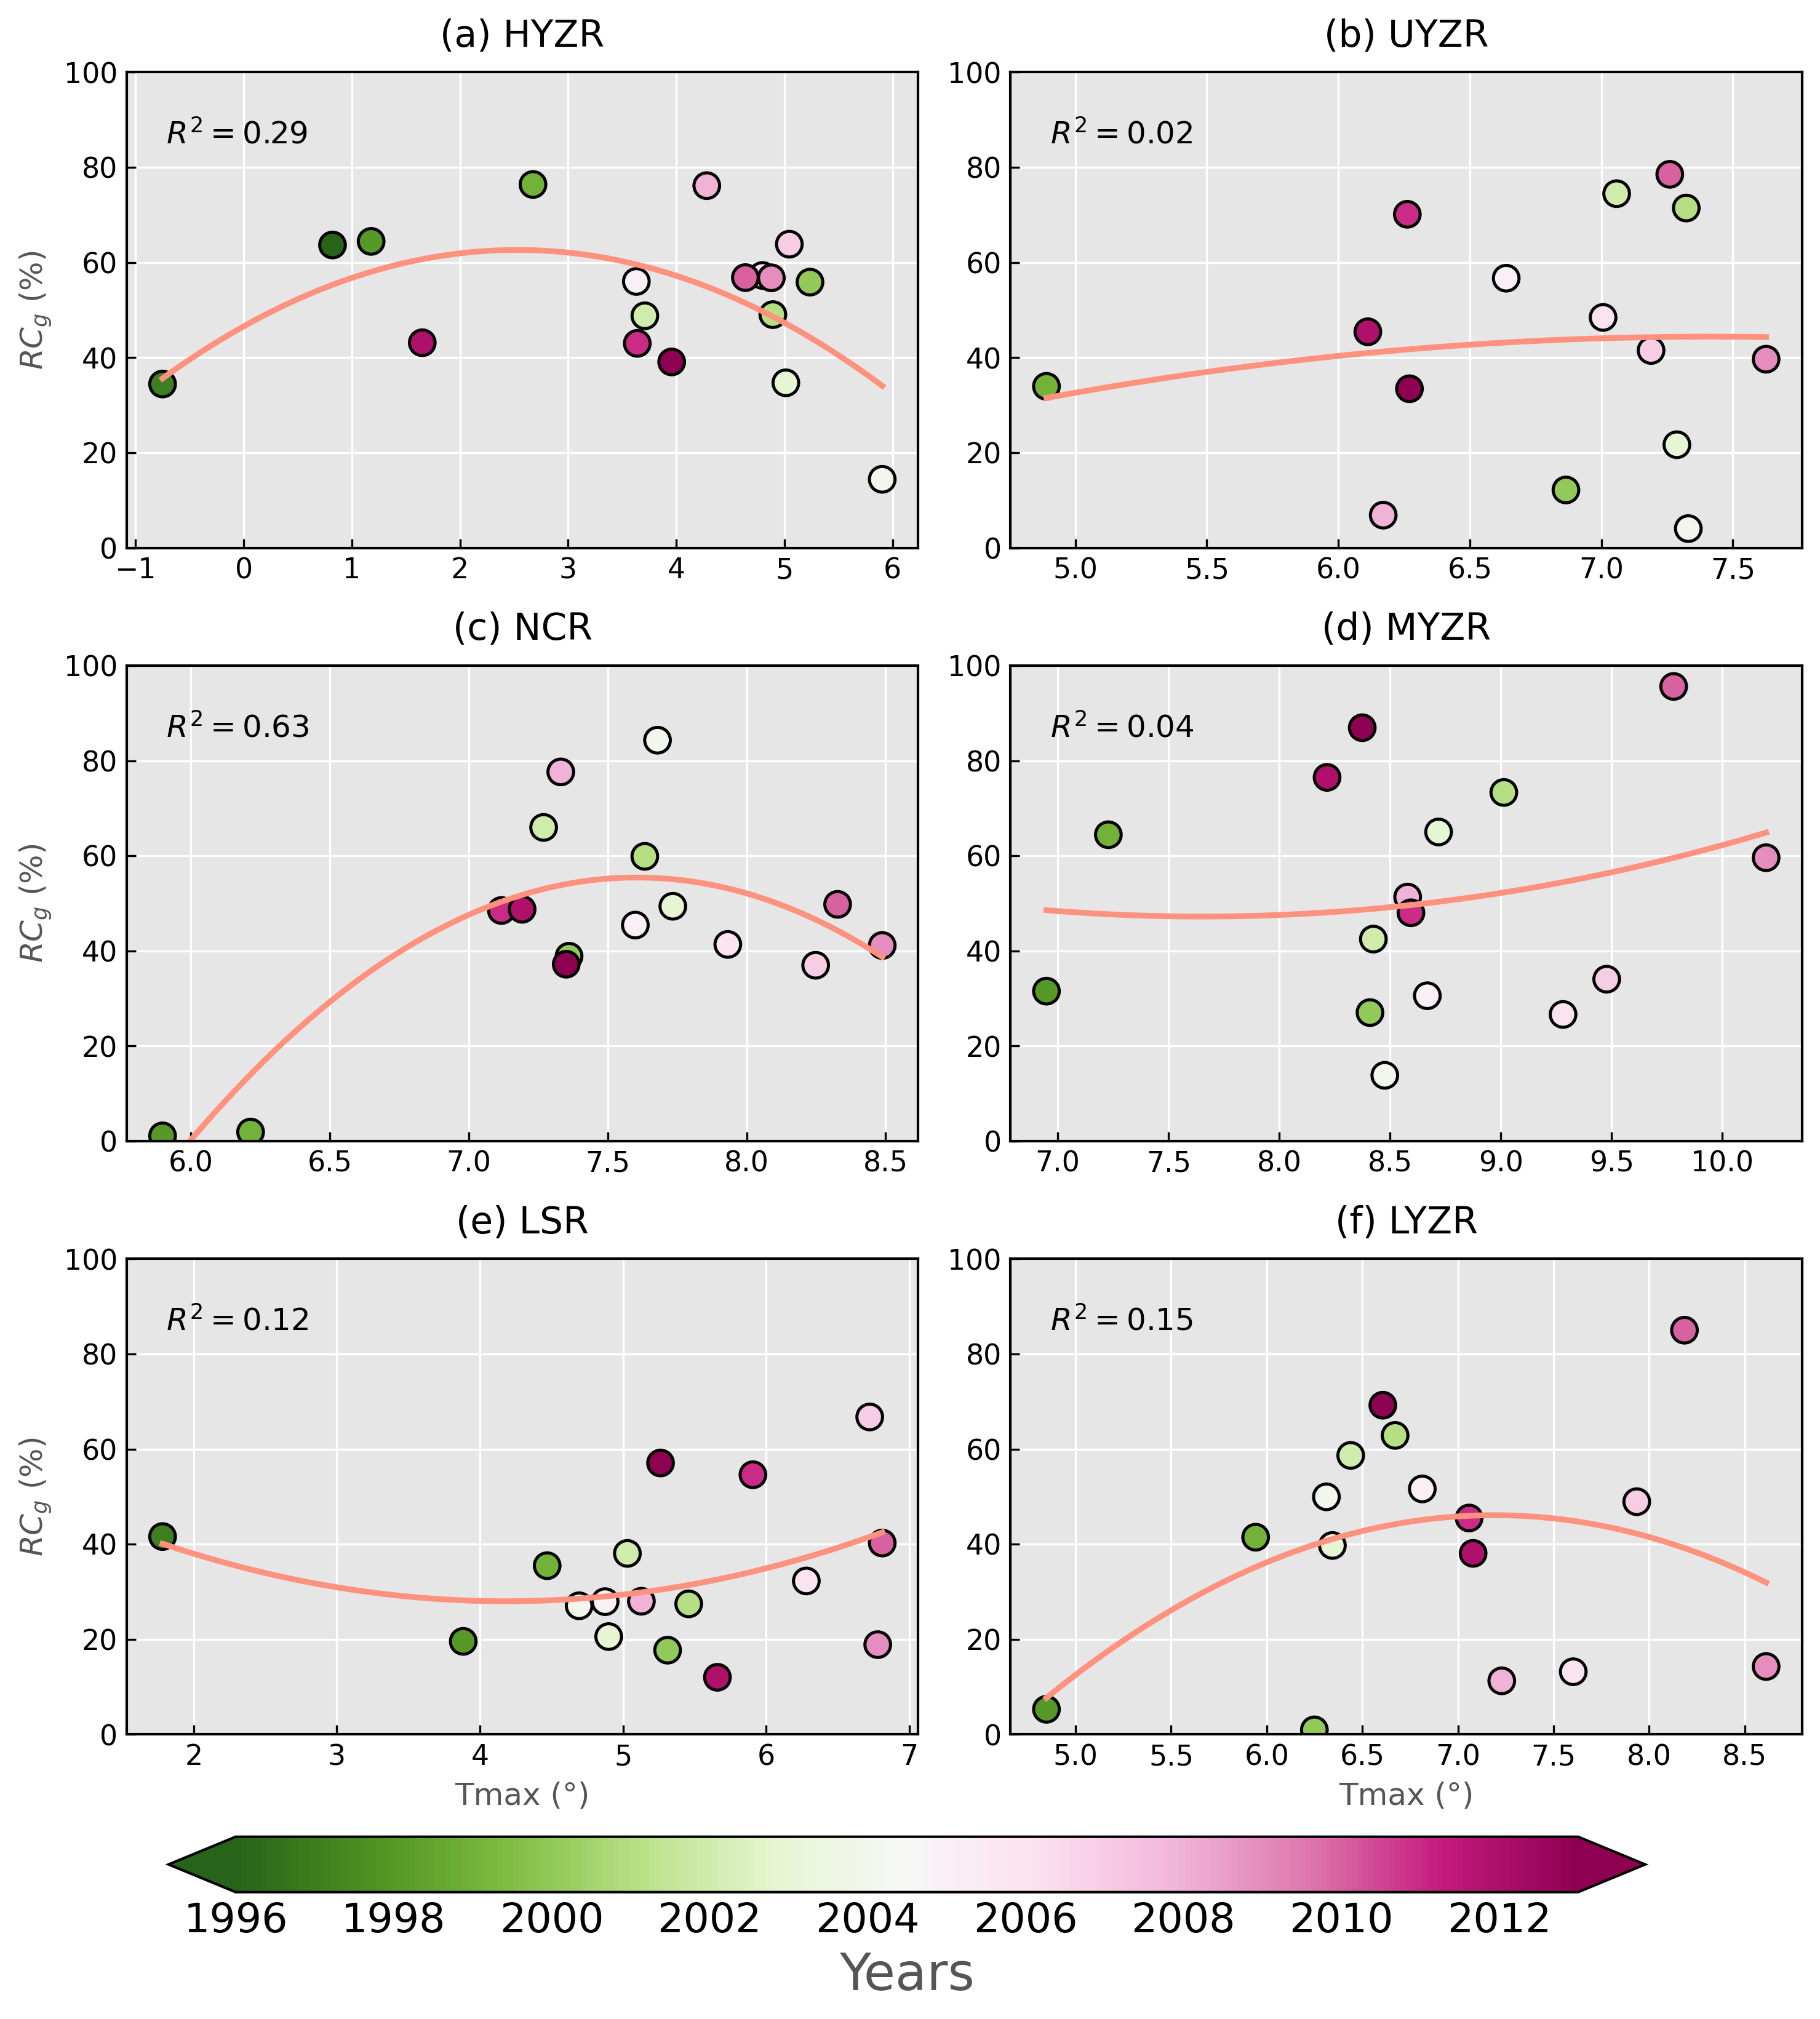
\includegraphics[width=8cm]{02-figures/peak-water-analysis.png}
    \captionsetup{labelformat=empty}
    \caption{Figure \ref{figS:warming-and-cryosphere}. The relationship between cryospheric contributions to water yield deviations ($\Delta WY_s(t)$) and annual mean 2m maximum air temperature ($T_{max}$) using the polynomial fitting. R square used to evaluate the fitting goodness is labelled in each panel.}
\end{figure*}

\nextreply{But, Figure 1 in \citetrev{huss2018global} recommended by the reviewer  shows the responses of cryospheric contributions to river flow under global warming. Based on this, we try to link cryospheric contributions with temperature changes, and find a nonlinear relationship between them (see Figure \ref{figS:warming-and-cryosphere}). Related revisions are described here.}

\revised{227--233}{Cryospheric contribution is also important for water yield regime shifts -- \ul{melt waters from glaciers and snow melting can alleviate water resources shortages, mainly caused by decreased precipitation in recent years} (Figure \ref{fig:attribution-direction}+\ref{figS:climate-directions}). This finding is also supported by observed glacier runoff data \citep{yao2010glacial} and several modeling studies \citep{lutz2014consistent, Zhang2020VariationOM, wang2021tp}. 
However, after glacier runoff reaches a maximum, defined as "peak water" \citep{gleick2010peak}, \ul{cryospheric mass loss cannot sustain the rising melt waters with atmospheric warming} (e.g. the HYZR basin in Figure \ref{figS:warming-and-cryosphere}), which is in agreement with \citet{huss2018global}.}

\revised{272--275}{In addition, our results clearly show that the melt waters from glaciers might have already surpassed the "peak water" (Figure \ref{figS:warming-and-cryosphere}), and the associated hydrological changes will substantially affect future water resources management. Thus, the projections of the occurrence time of "peak water" will be important in managing mountainous water resources.}

\sect{Abstract}

\point{I suggest you to remove useless adverbs such as “however, nevertheless, etc.”. Try to shorten the abstract a little bit, e.g., discarding not essential sentences or summarizing some concepts}
\reply{Thanks. We have rewritten the abstract (see below).}

\point{Line 15. Change “melt” with “loss”. Cryospheric changes can increase the amount of available water, e.g. in rock glaciers}
\reply{Thanks. We have rewritten the abstract (see below).}

\point{Line 18. Is it “stream head” correct word? I would delete the part “, as represented…downstream” in this sentence, useless for the abstract in my opinion.}
\reply{Thanks. We have deleted the useless sentence for the abstract to ensure it convey main information to readers (see below).}

\point{Line 19. Delete “we found that”}
\reply{Thanks. We have rewritten the abstract (see below).}

\point{Line 21. Delete “furthermore”}
\reply{Thanks. We have rewritten the abstract (see below).}

\point{Line 23. Delete “however”}
\reply{Thanks. We have deleted it (see below).}

\point{Line 25. Delete “nevertheless, we found that”}
\reply{Thanks. We have rewritten the abstract to strengthen its coherence (see below).}

\point{Line 28. What do you mean with “ecological restoration”?  I would remove this word as “water management” is enough in this context. Either, you can use the word “water governance”, which involves the management of water as well as the related ecosystems and resources}
\reply{Thanks for your advice. We deleted "ecological restoration" throughout the manuscript (see below).}

\nextreply{The revised abstract is as follows:}

\revised{1--12}{Although evidence of hydrological responses to climate is abundant, the reliable assessments of water yield (WY) over mountainous regions, such as the Upper Brahmaputra River (UBR) basin, remain unclear due to intensified cryospheric changes. 
Based on multi-station runoff observations, we examine long-term WY changes during 1982--2013 in the  UBR basin, and find there are in general hydrological regime shifts in the late 1990s; 
magnitude increases in WY range from $\sim$10\% to $\sim$80\%, while its directions reverse from upward to downward after the late 1990s.
Then, the double mass curve (DMC) technique is used to assess the effects of climate, vegetation, and cryosphere on WY changes. 
Results show that climate and cryosphere together contribute to over 80\% of magnitude increases of WY in the entire UBR basin, in which the role of vegetation is nearly negligible.
The combined effects, however, are either offsetting or additive, leading to slight or substantial magnitude increases, respectively. 
Climate change, particularly precipitation decrease leads to the downward WY trend in recent years,
while melt waters under global warming may alleviate the water shortage in some basins. 
Therefore, the combined effects of climate and cryosphere on WY should be considered in future water resources management over mountainous basins, particularly involving co-benefits between upstream and downstream regions.}

\sect{Introduction}

\point{Line 36. What do you mean with glacial snowmelt? Cryospheric drivers are snow and glaciers providing water across the melting process, i.e., glacier ice melt and snowmelt. 
Or do you mean the snowmelt occurring on the glacier surface? Please consider here the paper from Huss et al., 2017, which also includes the permafrost ice as a key component of the mountain cryosphere}
\reply{Thank you very much for pointing it out. We are so sorry for the misunderstanding and we use \textbf{"glaciers and snow melting"} throughout the revised manuscript.}

\point{Line 36. It is actually unclear to a layman what the Third Pole is. Please clearly and concisely define it the first time you name it}
\reply{Thanks. "Third pole" has the less role in the manuscript and also cause the confusion to the abbreviation of "turning point", so we have deleted it.}

\point{Line 52. “direction of change…” of what?}
\reply{Thanks. We have used the following expression to replace it:}

\revised{29--30}{For example, \citetrev{fan2015temperature} highlighted the important role of precipitation in WY increases in the Salween and Mekong River basins.}

\point{Line 54. “glacial snow”. See same comment of line 36.}
\reply{Thanks. We have used \textbf{"glaciers and snow melting"} throughout the manuscript.}

\point{Line 84-85. “a reference…modelling”. You already provided this sentence 8 lines earlier. Please avoid repetition.}
\reply{Thanks. We have deleted the repeated expressions.}

\sect{Results}

\point{Figure 3. I think the use of boxplots would greatly help interpretation.}
\reply{We have changed the figure to the boxplots to show the data distribution (Figure \ref{fig:magnitude-direction}).}

\point{Figure 5. I suggest you to provide the text and fitting lines for significant relationships only, to avoid figure overwhelming and help interpretation}
\reply{Thanks for your suggestions. We have created the figure to avoid overwhelming as following.}

\begin{figure*}[ht]
    \centering
    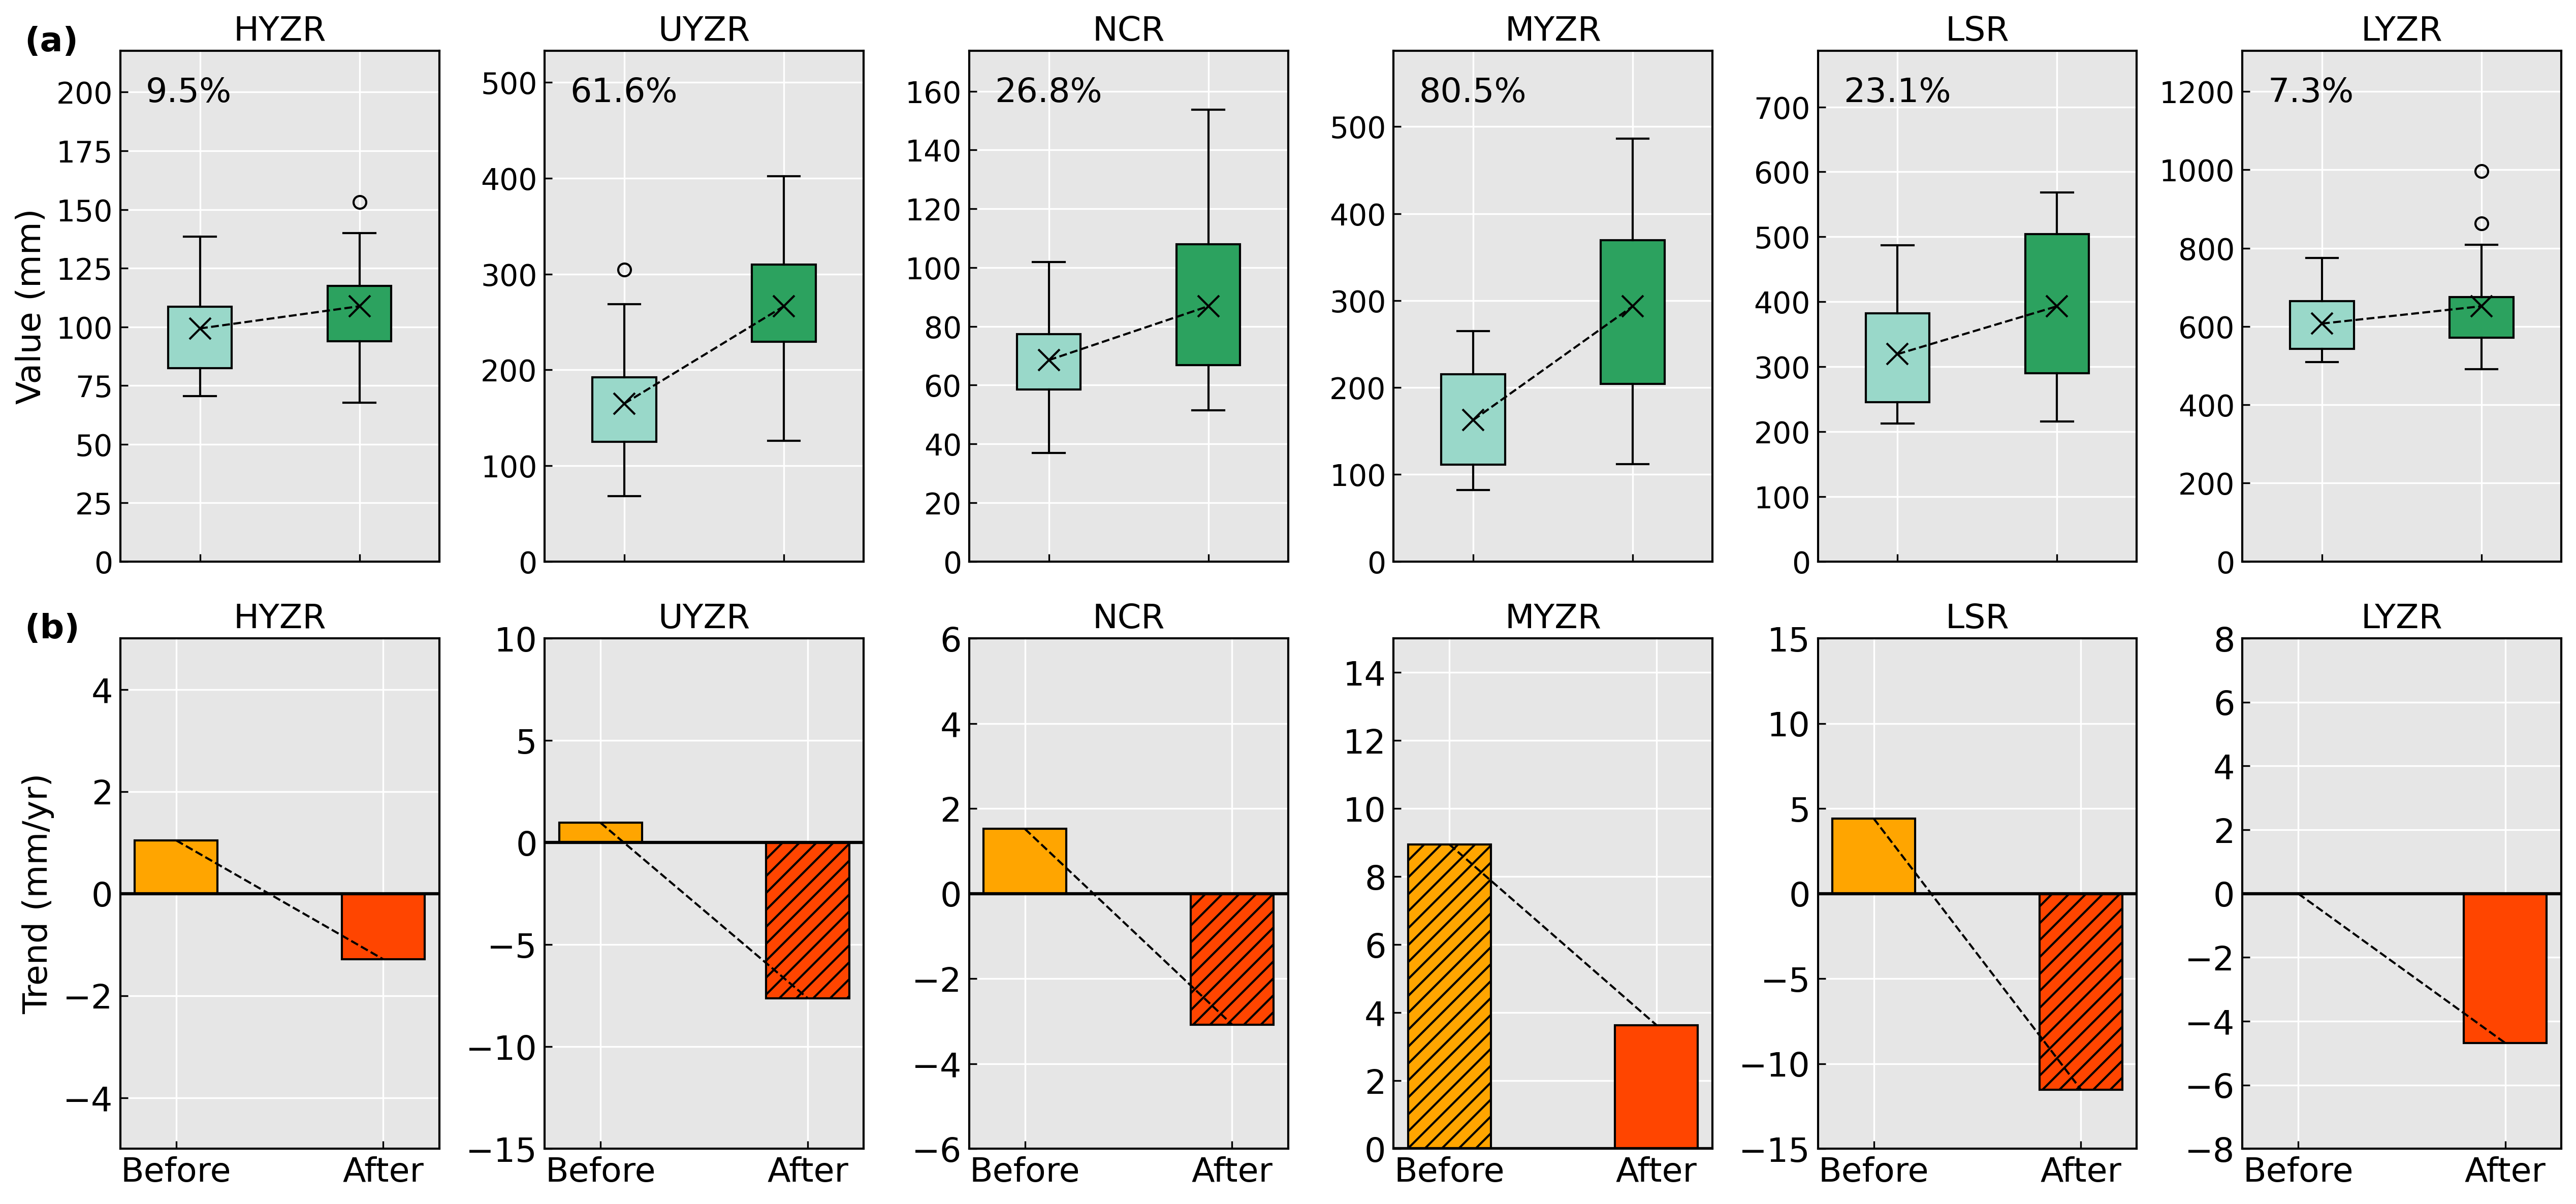
\includegraphics[width=8cm]{02-figures/magnitude_and_direction.png}
    \captionsetup{labelformat=empty}
    \caption
    {Figure \ref{fig:magnitude-direction}. Water yield regime shifts in the entire UBR basin. 
    (a) Magnitude of water yield changes. Black "x" signals show the mean of water yield in each boxplot.  
    (b) Direction of water yield changes. The black hatching represents the statistically significant trend (p $<$ 0.05).
    The color of boxes represents the period before (light color) and after (dark color) the turning point (TP).}
\end{figure*}

\begin{figure*}[ht]
    \centering
    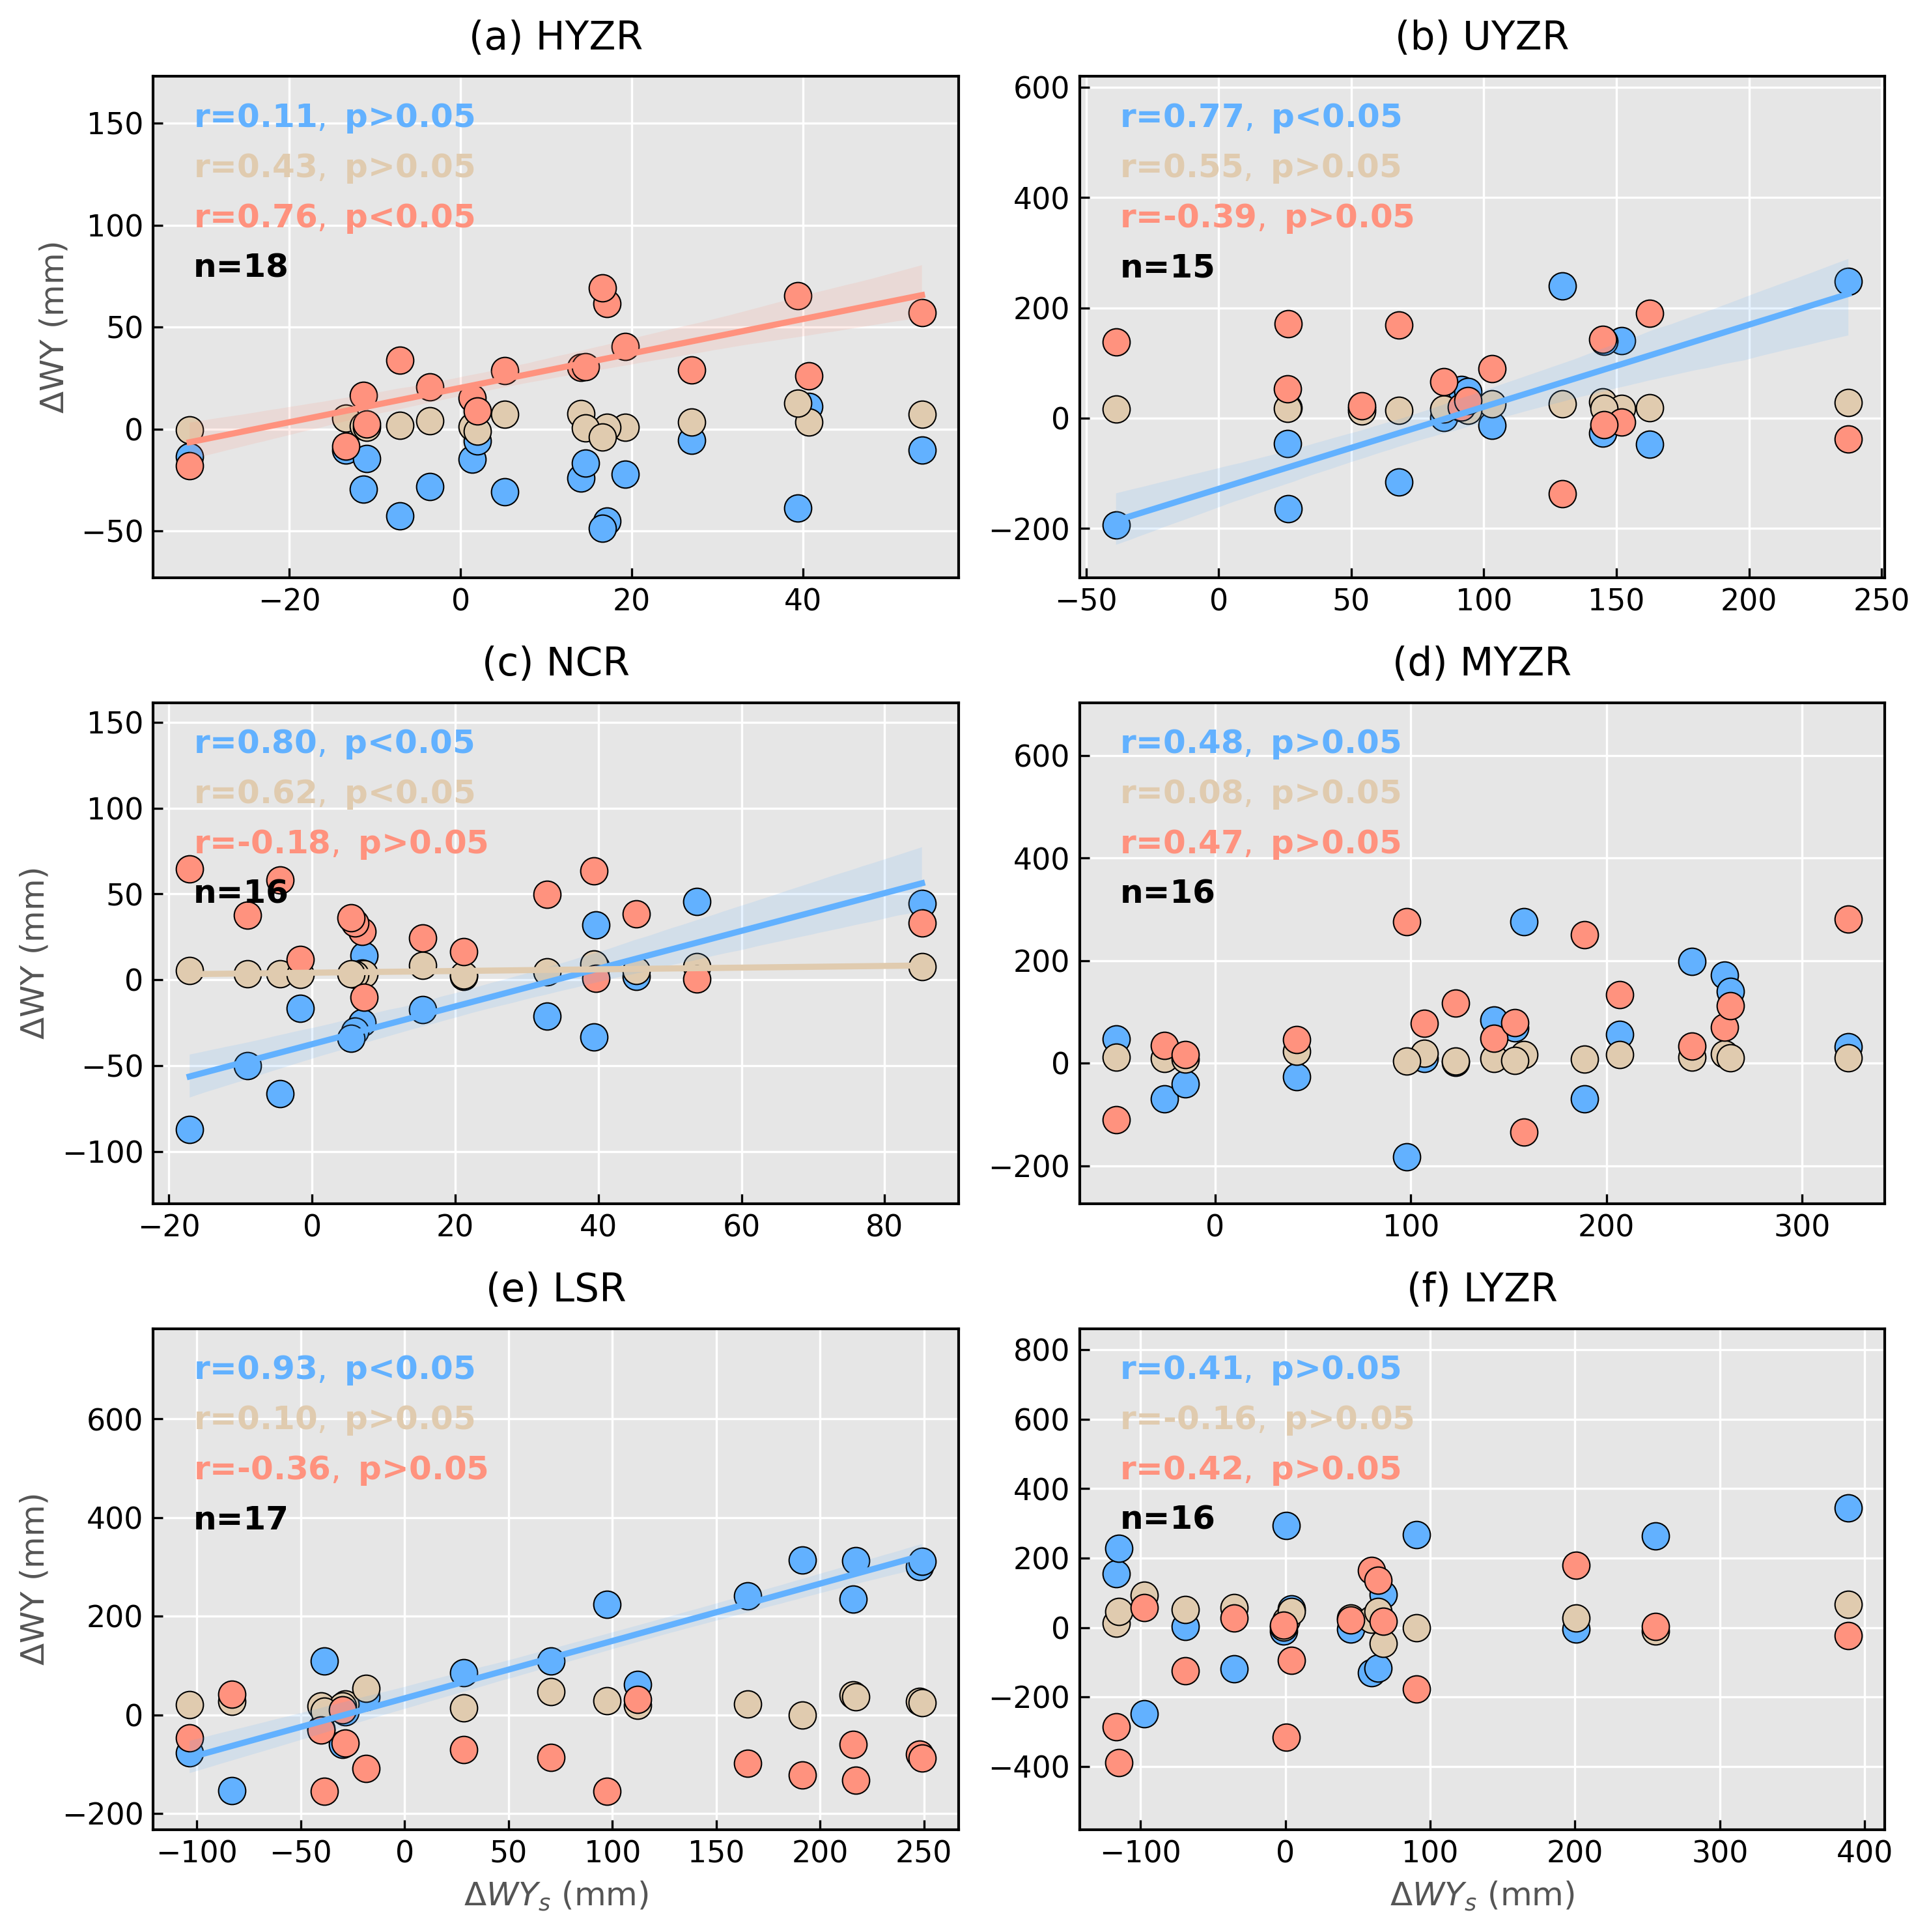
\includegraphics[width=6cm]{02-figures/contribution-relations.png}
    \captionsetup{labelformat=empty}
    \caption{Figure \ref{fig:attribution-direction}. The correlation between time series of total water yield deviation ($\Delta WY_s(t)$, x-axis) and its components (y-axis) caused by climate ($\Delta WY_c(t)$, blue point), vegetation ($\Delta WY_v(t)$, tan point), and cryosphere ($\Delta WY_g(t)$, red point), respectively.
    The fitting line and its 95\% confidence interval are shown only when p value $<$ 0.05. $n$ indicates the number of years after the TP, which is determined by the Pettitt method (See Table \ref{tab: table 1} and Figure \ref{fig:water-yield}c).}
\end{figure*}

\sect{Discussion}

\point{I think that an important work to be considered, that may help contextualising your storyline, would be Huss \& Hock (2018) providing the concept of “peak water”. I suggest you to reshape the discussion around this work. Your results clearly show that the upper Brahmaputra has already surpassed the Peak Water and is now in declining phase of hydrological changes associated with glacier loss. This conceptualisation would also help you to better discuss the turning points that different areas experienced during distinct years…the presence of these turning points should be better discussed, as it is one of the strengths of the chosen methodology.}
\reply{Thank you very much for your constructive comments. We have linked the results with "peak water", as revealed in \citeprev{huss2018global}.}

\revised{197--209}{In contrast to positive contributions of climate, we find that WY caused by cryosphere exhibits a negative association with reduced total WY deviations in recent years in the UYZR (r = -0.39, p $>$ 0.05) and LSR (r = -0.36, p $>$ 0.05) basins. 
The negative but weak relationship indicates that \ul{melt waters from cryospheric loss may compensate for low flow, and even mitigate water shortage risks}. 
Also, \ul{the compensating effect} from cryosphere is much stronger in the MYZR (r = 0.47, p $>$ 0.05), and together with climate contributions, contributes to the increasing WY trend (Figure \ref{fig:magnitude-direction}). 
Different from other regions, however, the HYZR basin shows a significantly positive relationship between cryospheric contributions and total WY deviations (r = 0.76, p $<$ 0.05), indicating that \ul{cryosphere instead of climate leads to the downward trend in headwaters.}
This signifies that in this region, \ul{cryospheric contributions have already passed a maximum supplying to river flow, due to decreased glaciers and snow under continuous warming}. 
The is further verified by the relationship of cryospheric contributions to total WY ($RC_g$) with temperature (Figure \ref{figS:warming-and-cryosphere}). 
In the HYZR basin, WY resulting from the cryosphere continues to \ul{increase with temperature until a maximum is reached, beyond which cryospheric contribution to total WY begins to decrease}.
In addition, \ul{the compensating effect of melt waters} can be seen clearly in the UYZR, MYZR and LSR basins, i.e., WY caused by cryospheric loss keeps a positive relationship with the increase of temperature, further supporting the higher correlation in these basins (Figure \ref{fig:attribution-direction}).}

\revised{227--233}{Cryospheric contribution is also important for water yield regime shifts -- melt waters from glaciers and snow melting can alleviate water resources shortages, mainly caused by decreased precipitation in recent years (Figure \ref{fig:attribution-direction}+\ref{figS:climate-directions}). This finding is also supported by observed glacier runoff data \citep{yao2010glacial} and several modeling studies \citep{lutz2014consistent, Zhang2020VariationOM, wang2021tp}. However, after glacier runoff reaches a maximum, defined as "peak water" \citep{gleick2010peak}, \ul{cryospheric mass loss cannot sustain the rising melt waters with atmospheric warming (e.g. the HYZR basin in this study)}, which is in agreement with \citet{huss2018global}.}

\revised{265--275}{Understanding the hydrological regime shifts and their causes in the high mountains are especially important in managing water resources, especially balancing the co-benefits between mountains and downstream lowlands \citep{viviroli2011climate}. 
In the study, the combined (offsetting or additive) effects from climate and cryosphere are detected (Figure \ref{fig:attribution-magnitude}), and further lead to either slight or substantial increases in WY in the entire UBR basin (Figure \ref{fig:magnitude-direction}a). 
The combined effects often hinder the roles of each driver in hydrological changes \citep{wei2018,zhang2021deforestation}, which should be considered when designing water management strategies in the large transboundary river system.
For example, the additive effect may be beneficial for mitigating droughts and water shortage during droughts, but it may exacerbate the flood risks due to increased precipitation and accelerated melting of the cryosphere in the future \citep{Immerzeel2013}.
In addition, our results clearly show that the melt waters from glaciers might have already surpassed the "peak water" (Figure \ref{figS:warming-and-cryosphere}), and the associated hydrological changes will substantially affect future water resources management. Thus, the projections of the occurrence time of "peak water" will be important in managing mountainous water resources.}

\point{Line 309-311. This is not true! See works from Huss and Hoch (2018), and in general the latest IPCC report on the ocean and the cryosphere, chapter dedicated to mountain environments…}
\reply{Thank you very much for pointing it out. In the original manuscript, we want to show that this study provides a more detailed analysis for water yield changes in the UBR basin. We have deleted it to avoid the confusion.}

\point{Line 330. Please change “retractration” with “loss” or “recession”. Also the sentence is unclear as written}
\reply{Thanks. We have rewritten this sentence.}

\revised{228--230}{..., melt waters from glaciers and snow melting can alleviate water resources shortages, ... This finding is also supported by observed glacier runoff data \citep{yao2010glacial} and several modeling studies \citep{lutz2014consistent, Zhang2020VariationOM, wang2021tp}.}

\point{Line 338. What do you mean with “ecological restoration”? It is unclear why this would help ecological restoration in particular. It is a general issue of water governance, after all, not just restricted to ecological restoration.}
\reply{Thank you very much for your comment. We use "water resources management" to indicate the implication of this study throughout the main text.}


\bibliographystylerev{copernicus}
\bibliographyrev{reference.bib}

\end{document}